\documentclass[12pt,english]{report}

%%%%%%%% Preamble %%%%%%%%%%%%
\usepackage[utf8]{inputenc}
\usepackage[T1]{fontenc}
\usepackage[english,french]{babel}
\usepackage{amsmath, amssymb, amsthm}
\usepackage{graphicx}
\usepackage{geometry} % Add this line
\usepackage{afterpage} % Add this line for better page control
\usepackage{rotating}
\usepackage[final]{pdfpages}
\usepackage{xcolor}
\usepackage{float}
\usepackage{subfigure}
\usepackage{parskip}
\usepackage{capt-of}
\usepackage{sidecap}
\sidecaptionvpos{figure}{c}
\usepackage{caption}
\usepackage{placeins}
\usepackage{lipsum}
\usepackage{commath}
\usepackage{cancel}
\usepackage{anysize}
\marginsize{2cm}{2cm}{2cm}{2cm}
\usepackage{appendix}
\usepackage{titlesec}
\usepackage{tikz}
\usetikzlibrary{shapes.geometric, arrows}
\setcounter{secnumdepth}{5}
\setcounter{tocdepth}{3}
\usepackage[colorlinks=true,plainpages=true,citecolor=blue,linkcolor=blue]{hyperref}
\usepackage{tikz}
\usetikzlibrary{shapes.geometric, arrows}
\usepackage{sectsty}
\usepackage{longtable}
\addto\captionsenglish{
    \renewcommand{\contentsname}{Table of Contents}
    \renewcommand{\listfigurename}{List of Figures}
    \renewcommand{\listtablename}{List of Tables}
    \renewcommand{\chaptername}{Chapter}
    \renewcommand{\appendixname}{Appendix}
}
% Colors for sections
\definecolor{sectioncolor}{HTML}{123456}
\definecolor{subsectioncolor}{HTML}{151B54}
\definecolor{subsubsectioncolor}{HTML}{0000FF}
\sectionfont{\color{sectioncolor}}
\subsectionfont{\color{subsectioncolor}}
\subsubsectionfont{\color{subsubsectioncolor}}

% Section numbering
\renewcommand{\thesection}{\arabic{section}}
\renewcommand{\thesubsection}{\thesection.\arabic{subsection}}
\renewcommand{\thesubsubsection}{\thesubsection.\arabic{subsubsection}}

% Table/Figure numbering
\usepackage{chngcntr}
\counterwithin{figure}{chapter}
\counterwithin{table}{chapter}
\renewcommand{\thefigure}{\arabic{figure}}
\renewcommand{\thetable}{\arabic{table}}

% Penalties for better formatting
\widowpenalty=10000
\clubpenalty=10000
\interlinepenalty=100

\usepackage{fancyhdr}
\pagestyle{fancy}
\fancyhf{}
\fancyhead[L]{\nouppercase{\leftmark}}  % English chapter titles
\fancyhead[R]{\footnotesize Year 2024-2025}
\fancyfoot[R]{\thepage}
\renewcommand{\footrulewidth}{0.4pt}


% Redefine plain page style (used for chapter start pages)
\fancypagestyle{plain}{
  \fancyhf{}
  \fancyfoot[R]{\thepage}
  \renewcommand{\headrulewidth}{0pt}
  \renewcommand{\footrulewidth}{0.4pt}
}

% Table-specific packages (optimized)
\usepackage{multirow}      % For merged cells
\usepackage{makecell}      % For line breaks inside cells
\usepackage{tabularx}      % For dynamic column width
\usepackage{booktabs}      % Professional lines
\usepackage{array}         % Column formatting
\usepackage{adjustbox}     % Table scaling
\renewcommand{\theadfont}{\bfseries} % Bold headers
\newcolumntype{Y}{>{\raggedright\arraybackslash}X} % New column type for tabularx

% For bullet points in tables
\newcommand{\tabitem}{\makecell[l]{\textbullet\hspace{0.5em}}}

% Glossaries
\usepackage[acronym]{glossaries}
\makeglossaries
\newacronym{ad}{AD}{Active Directory}

% Listings for code
\usepackage{listings}
\definecolor{dkgreen}{rgb}{0,0.6,0}
\definecolor{gray}{rgb}{0.5,0.5,0.5}
\definecolor{lightgray}{rgb}{0.95,0.95,0.95}

\lstdefinestyle{BashStyle}{
    language=bash,
    basicstyle=\footnotesize\ttfamily,
    keywordstyle=\color{blue},
    commentstyle=\color{gray},
    stringstyle=\color{red},
    backgroundcolor=\color{black!5},
    frame=single,
    rulecolor=\color{black!30},
    columns=fullflexible,
    breaklines=true,
    postbreak=\mbox{\textcolor{red}{$\hookrightarrow$}\space},
    showstringspaces=false,
    tabsize=2
    }

% Bibliography
\usepackage[
  backend=biber,
  style=numeric,
  defernumbers=true,
  sorting=none % <--- Add this to disable alphabetical sorting
]{biblatex}
\addbibresource{References.bib}

% Add the following lines to force order
\DeclareFieldFormat{labelnumberwidth}{[#1]}
\setlength{\biblabelsep}{0pt}

% Title
\title{Degree project}


%%%%%%%% Preamble ends %%%%%%%%%%%%
\begin{document}
\selectlanguage{english}  % Force English for the entire document

%%%%%%%%%%%%%%%%%%%%%%%%%%%%%%%% Cover Page %%%%%%%%%%%%%%%%%%%%%%%%%%%%%%%%%%%%%%%%%%%

																	
%%%%%%%%%%%%%%%%%%%% Cover page ends %%%%%%%%%%%%%%%%%%%%%%%%%%%%%%%%

%%%%%%%%%%%%%%%%%%%%%%%%%%%%%%%%%%%%%%%%%%%%%%%%%%%%%%%%%%%%%%%%

%%%%%%%%%%%%%%%%%%%%%%%%%%%%%%%%%%%%%%%%%%%%%%%%%%%%%%%%%%%%%%%%
\chapter*{Acknowledgments}
It is with immense gratitude that we dedicate this page to all those who have supported us in the successful completion of our final graduation project.

We would like to begin by expressing our heartfelt thanks to \textbf{3S}, the company that welcomed us and provided us with the opportunity to deepen our knowledge and gain practical experience. We are truly grateful for their trust and collaboration.

Our sincere appreciation goes to our professional supervisor,\textbf{ Mr. Mohamed AMIR Ben Soltane} , for his invaluable guidance, expertise, and encouragement throughout the duration of this project. His insights and feedback were instrumental in helping us overcome challenges and achieve our objectives.

We also extend our deepest gratitude to our academic supervisor, \textbf{Dr. Rim BOUHOUCH} , for her unwavering patience, constructive advice, and constant support. Her mentorship has been a source of inspiration and motivation for both of us.

Finally, we would like to thank \textbf{everyone} else who contributed, directly or indirectly, to the realization of this project. Your assistance and encouragement have been invaluable to us.

\tableofcontents
\newpage
\listoffigures
\newpage
\listoftables
\newpage
\chapter*{List of Acronyms}

\begin{table}[h!]
\label{tab:sdwan_acronyms}
\begin{tabularx}{\linewidth}{@{}>{\raggedright\arraybackslash}p{3cm}X@{}}
\toprule
\textbf{Acronym} & \textbf{Description} \\
\midrule
AAA & Authentication, Authorization, and Accounting \\
ACL & Access Control List – traffic filtering rules \\
BFD & Bidirectional Forwarding Detection – detects link failures quickly \\
BGP & Border Gateway Protocol – dynamic routing protocol \\
CA & Certificate Authority – entity that issues digital certificates \\
CPE & Customer Premises Equipment – hardware at the client side \\
DHCP & Dynamic Host Configuration Protocol – auto IP addressing \\
DNS & Domain Name System – translates domain names to IP addresses \\
GRE & Generic Routing Encapsulation – protocol for tunneling \\
IKE & Internet Key Exchange – key management protocol used with IPsec \\
LAN & Local Area Network \\
MPLS & Multiprotocol Label Switching – high-performance routing method \\
NAT & Network Address Translation – remaps IP addresses \\
OMP & Overlay Management Protocol – Cisco SD-WAN control protocol \\
OSPF & Open Shortest Path First – link-state routing protocol \\
QoS & Quality of Service – traffic prioritization mechanism \\
SD-WAN & Software-Defined Wide Area Network \\
SLA & Service Level Agreement – defines network performance guarantees \\
TCP & Transmission Control Protocol – connection-oriented transport \\
TLOC & Tunnel Locator – Identifies and establishes data plane tunnels \\
UDP & User Datagram Protocol – connectionless transport \\
vBond & Responsible for device authentication and orchestration \\
vEdge & Cisco SD-WAN edge router device \\
vManage & Graphical interface for centralized SD-WAN configuration and monitoring \\
vSmart & Centralized SD-WAN control and policy manager \\
VPN & Virtual Private Network \\
WAN & Wide Area Network \\
ZTP & Zero Touch Provisioning – automatic onboarding of devices \\
\bottomrule
\end{tabularx}
\end{table}
\chapter*{General Introduction}
\pagenumbering{arabic}
\addcontentsline{toc}{chapter}{General Introduction}
In today's digital era, companiess are constantly pressured to evolve their network infrastructures to keep up with cloud-first strategies, remote work models, and real-time applications. Traditional Wide Area Networks (WANs), once the backbone of enterprise connectivity, are now showing signs of strain, from high costs to limited scalability and rigid architectures.

This is where Software-Defined Wide Area Networking (SD-WAN) comes into play. More than just a technology upgrade, SD-WAN represents a strategic shift toward smarter, faster, and more agile networking. It enables organizations to leverage cost-effective Internet links, dynamically route traffic according to application needs, and maintain centralized control across distributed branches.

This report documents the implementation of the Cisco Viptela SD-WAN solution as part of a final-year academic project carried out at Standard Sharing Software (3S), a leading IT integrator in Tunisia. The goal was to simulate a real-world deployment scenario, covering device-level configuration, certificate authentication, policy definition, and performance validation, while gaining hands-on experience with one of the most advanced SD-WAN platforms available.

The journey began with an overview of the SD-WAN fundamentals and an evaluation of available solutions. We then moved into CLI-based configuration, centralized management through vManage, and finally testing to ensure everything worked as expected.

Through this project, our goal was not only to implement a functional SD-WAN architecture but also to understand its impact on modern enterprise networks, preparing ourselves for the evolving world of software-defined infrastructure.

\chapter{SD-WAN Fundamentals, Market Solutions and Selection Rationale}
\section{Introduction}
This chapter presents the foundational context, core concepts, and solution selection process for implementing an SD-WAN architecture at Standard Sharing Software (3S). It begins with an overview of 3S as a strategic IT partner in Tunisia, followed by an explanation of the challenges posed by traditional networking models like MPLS.

An in-depth introduction to SD-WAN is provided, covering its architecture, benefits, and migration strategies. The methodology used throughout the project, a practical, test-driven approach inspired by Agile principles, is also detailed.

Finally, this chapter explores the various SD-WAN platforms evaluated, including Fortinet, Versa Networks, and Cisco Viptela. It concludes with a justification for selecting Cisco Viptela based on its scalability, centralized management capabilities, and robust security features. 
\section{Overview of the Host Organization}
3S is a technology group that has established itself as a leader in integrated IT solutions and value-added services over its 36 years of existence. Operating in Tunisia and North Africa, the company specializes in delivering innovative and future-oriented technological infrastructure and network services. With decades of experience under its belt, 3S has grown into a trusted name by forging strategic alliances with globally renowned partners such as Cisco, Microsoft, IBM, Fortinet and EMC. These partnerships have allowed 3S to remain at the forefront of technological advancements and deliver cutting-edge solutions tailored to the needs of modern businesses\cite{ref1}.
\section{The Challenge}
The rapid adoption of cloud technologies and online services has introduced significant challenges for organizations still reliant on traditional networking solutions such as Multi-Protocol Label Switching (MPLS). These legacy systems are often associated with high costs, limited flexibility, and complex management requirements. As businesses increasingly shift to cloud-based applications and embrace remote work models, the demand for more efficient, scalable, and agile networking solutions has become paramount. In response, many enterprises are turning to SD-WAN technology to optimize both the performance and manageability of their wide-area networks. This transition highlights the need for organizations to carefully evaluate how they can move away from rigid, expensive MPLS-based infrastructures toward more flexible, cost-effective, and high-performance SD-WAN solutions\cite{ref2}.

\subsection{3S as a Strategic Partner}

It is within this context that 3S, a leader in deploying SD-WAN solutions in Tunisia, was selected as a strategic partner by one of its clients to implement this transformative technology across their network infrastructure. By adopting SD-WAN, the client aims to achieve greater network agility, reduce operational expenses, and enhance overall performance, objectives that seamlessly align with the expertise of 3S and the mission-driven approach to networking innovation\cite{ref1}.

\section{Introduction to SD-WAN}
SD-WAN , short for Software-Defined Wide Area Network , is a modern networking approach that brings agility and control back into enterprise connectivity. Unlike older WAN models that rely heavily on expensive, dedicated circuits routed through central data centers, SD-WAN allows branch offices to connect directly to the internet using high-speed broadband links.

This shift not only cuts down on costs but also improves performance, especially for cloud-based services. Instead of forcing traffic through a central hub, SD-WAN intelligently routes it based on real-time conditions, application needs, and security policies.

One of its standout features is centralized management. IT teams can configure and monitor devices across multiple locations from a single dashboard, reducing manual work and minimizing errors. For growing businesses with distributed operations, this kind of flexibility is a game-changer.

In short, SD-WAN isn’t just a technology upgrade, it's a strategic move toward smarter, faster, and more responsive networking\cite{ref3}.
\begin{figure}[H]
    \centering
    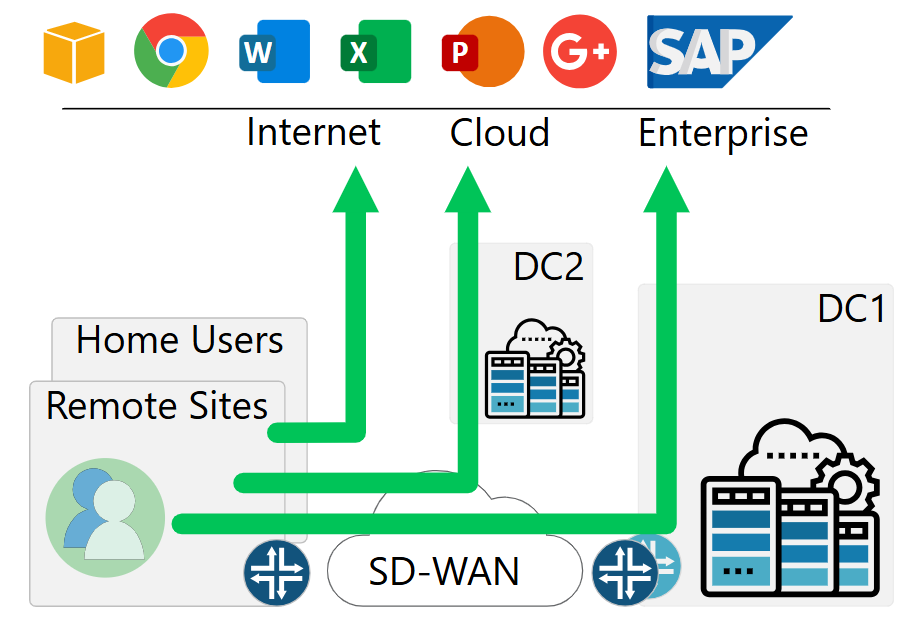
\includegraphics[width= 1 \textwidth]{chapter1/sdwan-intro.png}
    \caption{Software-Defined WAN architecture \cite{ref3}}
    \label{fig: Software-Defined WAN architecture}
\end{figure}
\subsection{Centralized Management in SD-WAN}
A standout feature of SD-WAN is its centralized management capability. Rather than manually configuring each WAN device across multiple locations, administrators can deploy configurations and enforce access policies from a single, unified interface. This ensures consistency across the network while streamlining operations and reducing the risk of human error\cite{ref2}.
\subsection{Core Architecture of SD-WAN}
At its foundation, SD-WAN operates by leveraging Virtual Private Networks (VPNs) over enterprise-grade Internet Protocol (IP) connections, supplemented by high-speed broadband and wireless services. This architecture supports cost-effective application management, particularly for cloud-hosted workloads. One of the most significant advantages of SD-WAN is its ability to dynamically route traffic along the most optimal path based on real-time criteria such as network conditions, security policies, and Quality of Service (QoS) requirements for specific applications\cite{ref3}.
\subsection{The Importance of SD-WAN in Modern Business}
In today’s rapidly evolving digital landscape, organizations are increasingly adopting cloud-based technologies to enable modern workflows and improve operational agility. These innovations are reshaping industries and redefining how businesses operate and compete. A critical component of this transformation is ensuring that remote employees have secure, fast, and reliable access to essential applications and data from any location\cite{ref3}.
\section{Challenges with Traditional Networking Models}
Traditional networking models, such as hub-and-spoke designs reliant on private links, often fall short in meeting these demands. These legacy systems struggle to handle the growing volume of bandwidth-intensive tasks, including video conferencing, online training sessions, and large-scale data transfers. Additionally, IT teams face the dual challenge of optimizing network performance while minimizing costs associated with hardware upgrades and frequent reconfigurations. This issue is especially pronounced for enterprises with distributed operations spanning multiple branches, stores, or offices across vast geographic regions\cite{ref3}.
\begin{figure}[H]
    \centering
    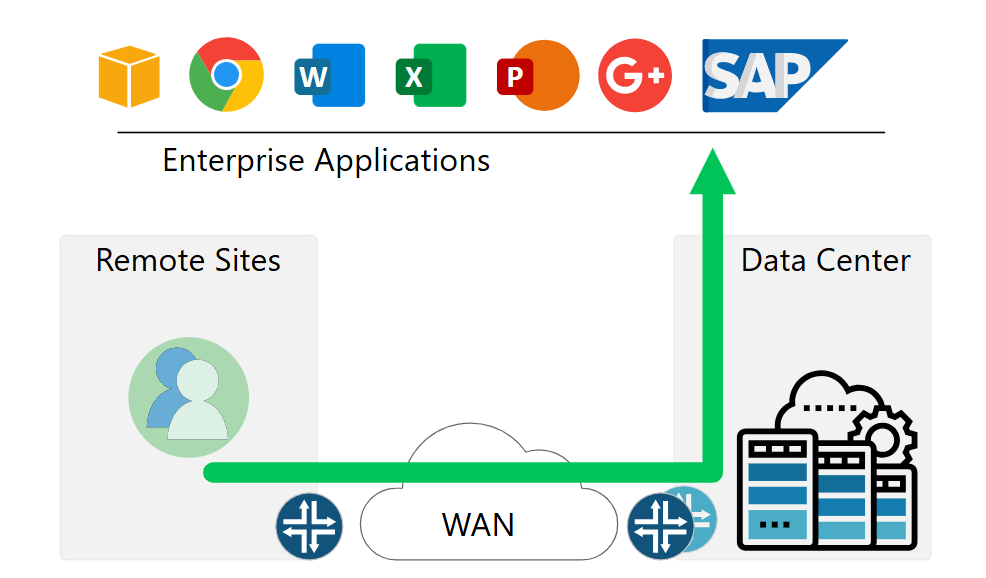
\includegraphics[width= 1 \textwidth]{chapter1/trad-wan.png}
    \caption{Traditional WAN architecture\cite{ref3}}
    \label{fig: Traditional WAN architecture}
\end{figure}

\subsection{{The Difference Between WAN and SD-WAN}}
Traditional Wide Area Networks (WANs) have long served as the backbone of enterprise networking, enabling organizations to connect geographically dispersed sites. However, enhancing these networks often required significant investments in specialized infrastructure, advanced equipment, and dedicated teams to configure and maintain them. Fine-tuning the equipment to ensure optimal performance could take days or even weeks, making the process both time-intensive and costly. Moreover, traditional WANs were inherently rigid, limiting an organization’s ability to adapt quickly to changing business needs.

In contrast, Software-Defined Wide Area Networking (SD-WAN) addresses these challenges by simplifying network complexity and reducing costs. SD-WAN allows organizations to leverage widely available, cost-effective Internet Service Provider (ISP) connections instead of relying on expensive proprietary solutions like Multi-Protocol Label Switching (MPLS). By utilizing standard broadband connections, businesses can achieve reliable wide-area networking without the need for dedicated infrastructure. Advanced SD-WAN solutions further enhance performance by intelligently combining and optimizing multiple connection types and ISPs, ensuring consistent and high-quality connectivity across all sites.

Another significant advantage of SD-WAN is its centralized management capabilities. Administrators can configure and manage all network sites from a single interface, eliminating the need to manually adjust individual devices. This centralized approach provides comprehensive visibility into the entire network, enabling administrators to monitor traffic patterns, detect anomalies, and respond swiftly to potential issues\cite{ref4}.
\begin{figure}[H]
    \centering
    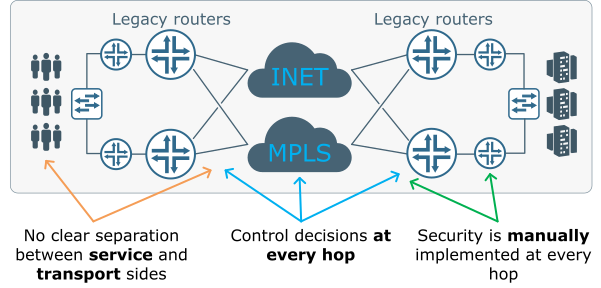
\includegraphics[width= 0.7 \textwidth]{chapter1/legacy-wan.png}
\end{figure}
\begin{figure}[H]
    \centering
    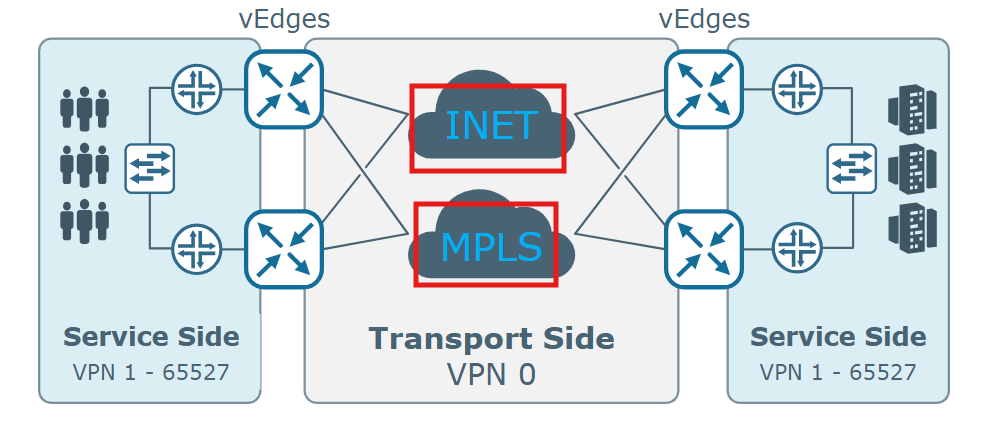
\includegraphics[width= 0.7 \textwidth]{chapter1/sdwan-paths.png}
    \caption{Traditional WAN vs. SD-WAN Architecture \cite{ref4}}
    \label{fig: Traditional WAN vs. SD-WAN Architecture}
\end{figure}

\subsection{The Benefits of SD-WAN}
Many organizations, including businesses and government agencies, are adopting SD-WAN to move away from the slow and costly MPLS lines that have traditionally dominated networking. While the immediate appeal lies in cost savings, the true value of SD-WAN extends far beyond reduced expenses. Key benefits include lower connectivity costs, improved performance for cloud applications, enhanced network resilience, greater operational agility, and optimized resource utilization.
    \begin{itemize}

 \item \textbf{Reduced Connectivity Costs :} SD-WAN dramatically lowers implementation expenses by replacing expensive MPLS lines with more affordable broadband services such as fiber optics, ADSL, or mobile wireless technologies. This shift not only reduces costs but also provides faster and more flexible connectivity options, empowering organizations to scale their networks efficiently.

 \item \textbf{Enhanced Performance for Cloud Applications :} Traditional WAN architectures often struggle with latency and inefficiencies when handling cloud-based applications. SD-WAN addresses this by enabling direct internet access for cloud services, minimizing delays and ensuring faster, more reliable application performance. Additionally, SD-WAN allows organizations to easily add supplementary links to sites requiring higher capacity, further enhancing performance.

 \item \textbf{Resilience Through Multiple Links :} Unlike traditional WANs, which typically rely on a single incoming link per site—a potential single point of failure—SD-WAN supports multiple links from different ISPs. This redundancy ensures continuous connectivity even if one link fails, significantly improving network reliability and reducing the risk of downtime.

 \item \textbf{Greater Agility :} In today’s fast-paced business environment, the ability to deploy networks quickly and securely is crucial. SD-WAN enables organizations to rapidly establish new branches or expand operations by leveraging the most suitable ISPs for each location. This flexibility accelerates deployment timelines while maintaining robust security and reliability.

 \item \textbf{Optimized Resource Utilization :} SD-WAN intelligently assigns critical applications to the most appropriate links—whether internal connections or internet-based pathways—based on predefined Quality of Service (QoS) requirements. This ensures that resources are allocated efficiently, balancing performance and cost-effectiveness to meet specific business needs. By prioritizing mission-critical traffic, SD-WAN maintains high productivity levels while keeping operational expenses under control\cite{ref3}.
\end{itemize}
\subsection{Migrating to SD-WAN}

Moving from a traditional WAN setup to an SD-WAN environment might sound straightforward, but it’s a process that requires careful planning and execution. While SD-WAN promises better performance and lower costs, the migration itself comes with its own set of challenges.

Here's how we approached it:
\begin{itemize}
    \item \textbf{Know Your Team’s Strengths:} Rolling out SD-WAN involves deploying new devices across multiple sites, which isn’t something you want to rush or leave to chance. We took time to assess our team’s capabilities and ensured everyone was comfortable with the tools and processes involved. When needed, we brought in extra expertise to avoid bottlenecks.

    \item \textbf{Understand the Current Setup:} Before making any changes, we mapped out the existing network. Understanding current traffic flows, critical applications, and routing practices gave us a clear picture of what to expect — and helped us avoid surprises during the switch.

    \item \textbf{Build a Realistic Plan:} A solid plan was essential. We outlined each phase of the rollout, including timelines, responsibilities, and expected outcomes. We prioritized which branches would be migrated first and decided which type of connectivity (broadband, LTE, etc.) would be best suited for each location.

    \item \textbf{Give Yourself Time:} Rushing the migration can lead to configuration errors or service disruptions. We allowed enough time for testing, troubleshooting, and user training. Unexpected issues — like unknown dependencies or performance inconsistencies — are common, so having some buffer time really helps.

    \item \textbf{Keep It Simple Where You Can:} Many organizations operate on complex, multi-vendor environments. To make things easier, we looked for ways to standardize configurations and consolidate tools wherever possible. This simplified both the migration and long-term maintenance.
\end{itemize} 
By following these steps, we were able to transition smoothly into the new architecture while ensuring minimal downtime and maximum efficiency\cite{ref3}.

\section{Methodology and Planning}
\label{sec:methodology}

Any IT project, regardless of its size or objectives, requires careful organization throughout its lifecycle. Modeling plays a key role by simplifying and representing the project in an accessible format. It also helps identify complexity levels and anticipate potential challenges.

In this context, our team of two followed \textbf{a practical, iterative, and test-driven methodology} that allowed us to build and refine the SD-WAN implementation step by step. Although we drew inspiration from Agile principles, particularly the emphasis on iteration, testing, and adaptability, we adapted the approach to suit our specific environment and constraints.

\subsection{Choice of Methodology}

After evaluating different strategies, we chose to apply a flexible and incremental methodology, focusing on
\begin{itemize}
    \item Breaking down tasks into manageable components
    \item Implementing configurations incrementally
    \item Testing after every major change
    \item Refining configurations based on results
\end{itemize}
This allowed us to ensure stability, make real-time adjustments, and improve the system gradually while gaining valuable hands-on experience.
\subsubsection{Traditional Approach}

The traditional or ``Waterfall'' methodology follows a linear sequence:

requirements $\rightarrow$ design $\rightarrow$ implementation $\rightarrow$ testing $\rightarrow$ maintenance.

Each phase must be completed before moving on to the next. While this works well for large-scale or fixed-scope projects, it lacks flexibility when frequent adjustments are needed.

In our case, this kind of rigid structure wasn’t suitable due to the dynamic nature of the implementation and the need for constant tuning and validation \cite{ref5}.

\subsubsection{Agile Approach}

Agile methodologies emphasize collaboration, iteration, and adaptability. They allow teams to break work into smaller cycles, delivering incremental improvements and incorporating feedback regularly.

Although Agile is often associated with software development, its core principles align well with how we approached this project. As a small team, we found that breaking tasks into smaller chunks and reviewing progress frequently helped us stay aligned and responsive to changes\cite{ref6}.

\subsubsection{Overview of the Scrum Methodology}

Scrum is a popular Agile framework used in many IT projects. It organizes work into short periods called \emph{sprints}, usually lasting two to four weeks. At the end of each sprint, the team reviews progress, adjusts priorities, and plans the next steps.

\begin{figure}[H]
    \centering
    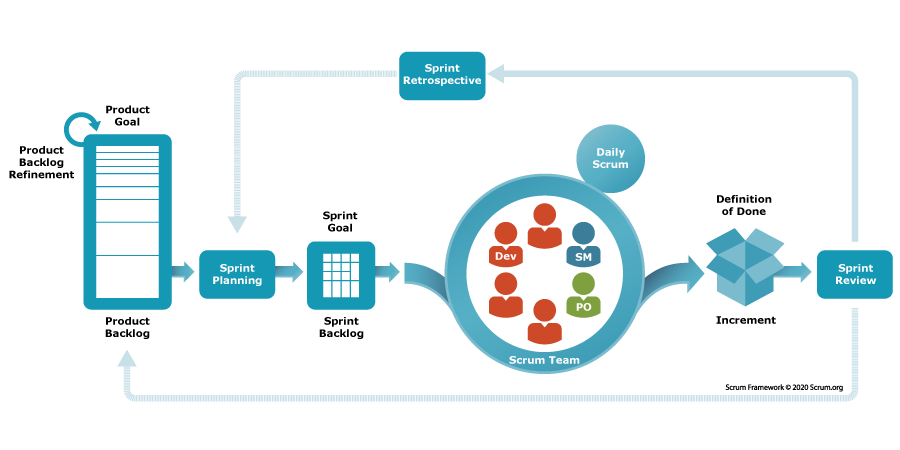
\includegraphics[width= 1\textwidth]{chapter1/scrum.png}
    \caption{Scrum Methodology \cite{ref7}}
    \label{fig: Scrum Methodology}
\end{figure}

While we didn't follow Scrum in a strict sense — without formal sprint planning meetings or daily stand-ups — we did adopt some of its core ideas:

\begin{itemize}
    \item We worked in small, manageable chunks.
    \item We tested frequently and made adjustments based on results.
    \item We reviewed progress continuously and refined configurations accordingly.
\end{itemize}

This lightweight Agile-inspired method suited our small team perfectly and allowed us to maintain flexibility while ensuring quality and consistency\cite{ref7}.

\subsection{Implementation Workflow}

To better illustrate the methodology we followed, the figure below shows the step-by-step workflow during the SD-WAN implementation:

\begin{figure}[H]
    \centering
    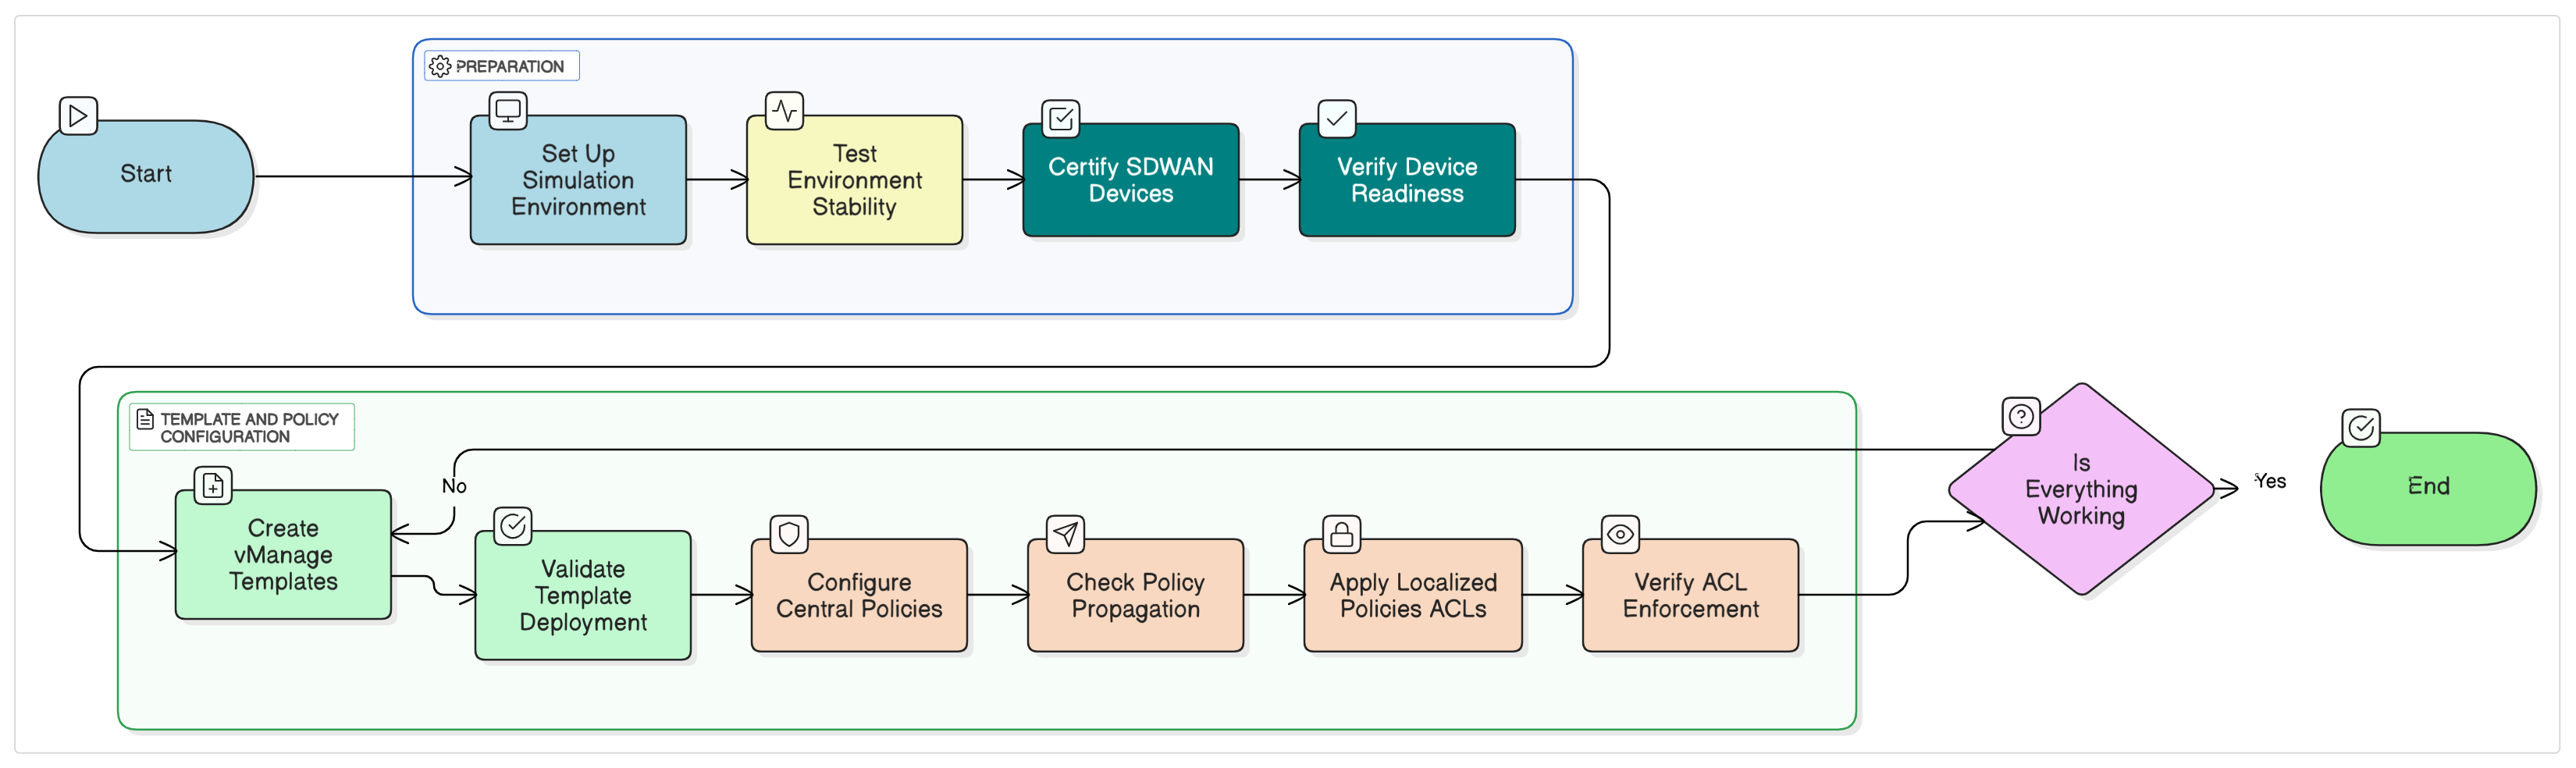
\includegraphics[width= 1\textwidth]{chapter1/diagram-export-17-05-2025-18_04_52.png}
    \caption{Used Methodology}
    \label{fig: Used Methodology}
\end{figure}
\section{The Various SD-WAN Solutions Available}
The SD-WAN market is rich with diverse solutions, each built on similar foundational principles but offering distinct features tailored to specific organizational requirements. Prominent players in this space include Versa Networks’ Secure SD-WAN, Fortinet’s Secure SD-WAN, and Cisco’s Viptela SD-WAN. These providers bring unique strengths to the table, addressing challenges such as security, scalability, and operational efficiency in different ways.

\subsection{Secure SD-WAN by Fortinet}
Fortinet’s Secure SD-WAN stands out as a cutting-edge solution delivered through its FortiGate platform, specifically designed for cloud-driven enterprises seeking robust security and global network visibility. By automating critical processes for both Network Operations Centers (NOCs) and Security Operations Centers (SOCs), Fortinet ensures seamless self-healing capabilities and policy orchestration. The integration of security, routing, and SD-WAN functionalities accelerates threat detection and network convergence, creating a more cohesive enterprise network.

A key differentiator of Fortinet’s solution is its incorporation of a next-generation firewall (FortiGate), advanced routing, and SD-WAN capabilities into a single platform. This unified approach not only enhances security speed but also improves operational efficiency through deep analytics, which optimize user experience and minimize downtime. Additionally, the platform’s global visibility empowers distributed teams to operate smoothly, while adaptive policies ensure security remains aligned with evolving business needs \cite{ref8}.
\begin{figure}[H]
    \centering
    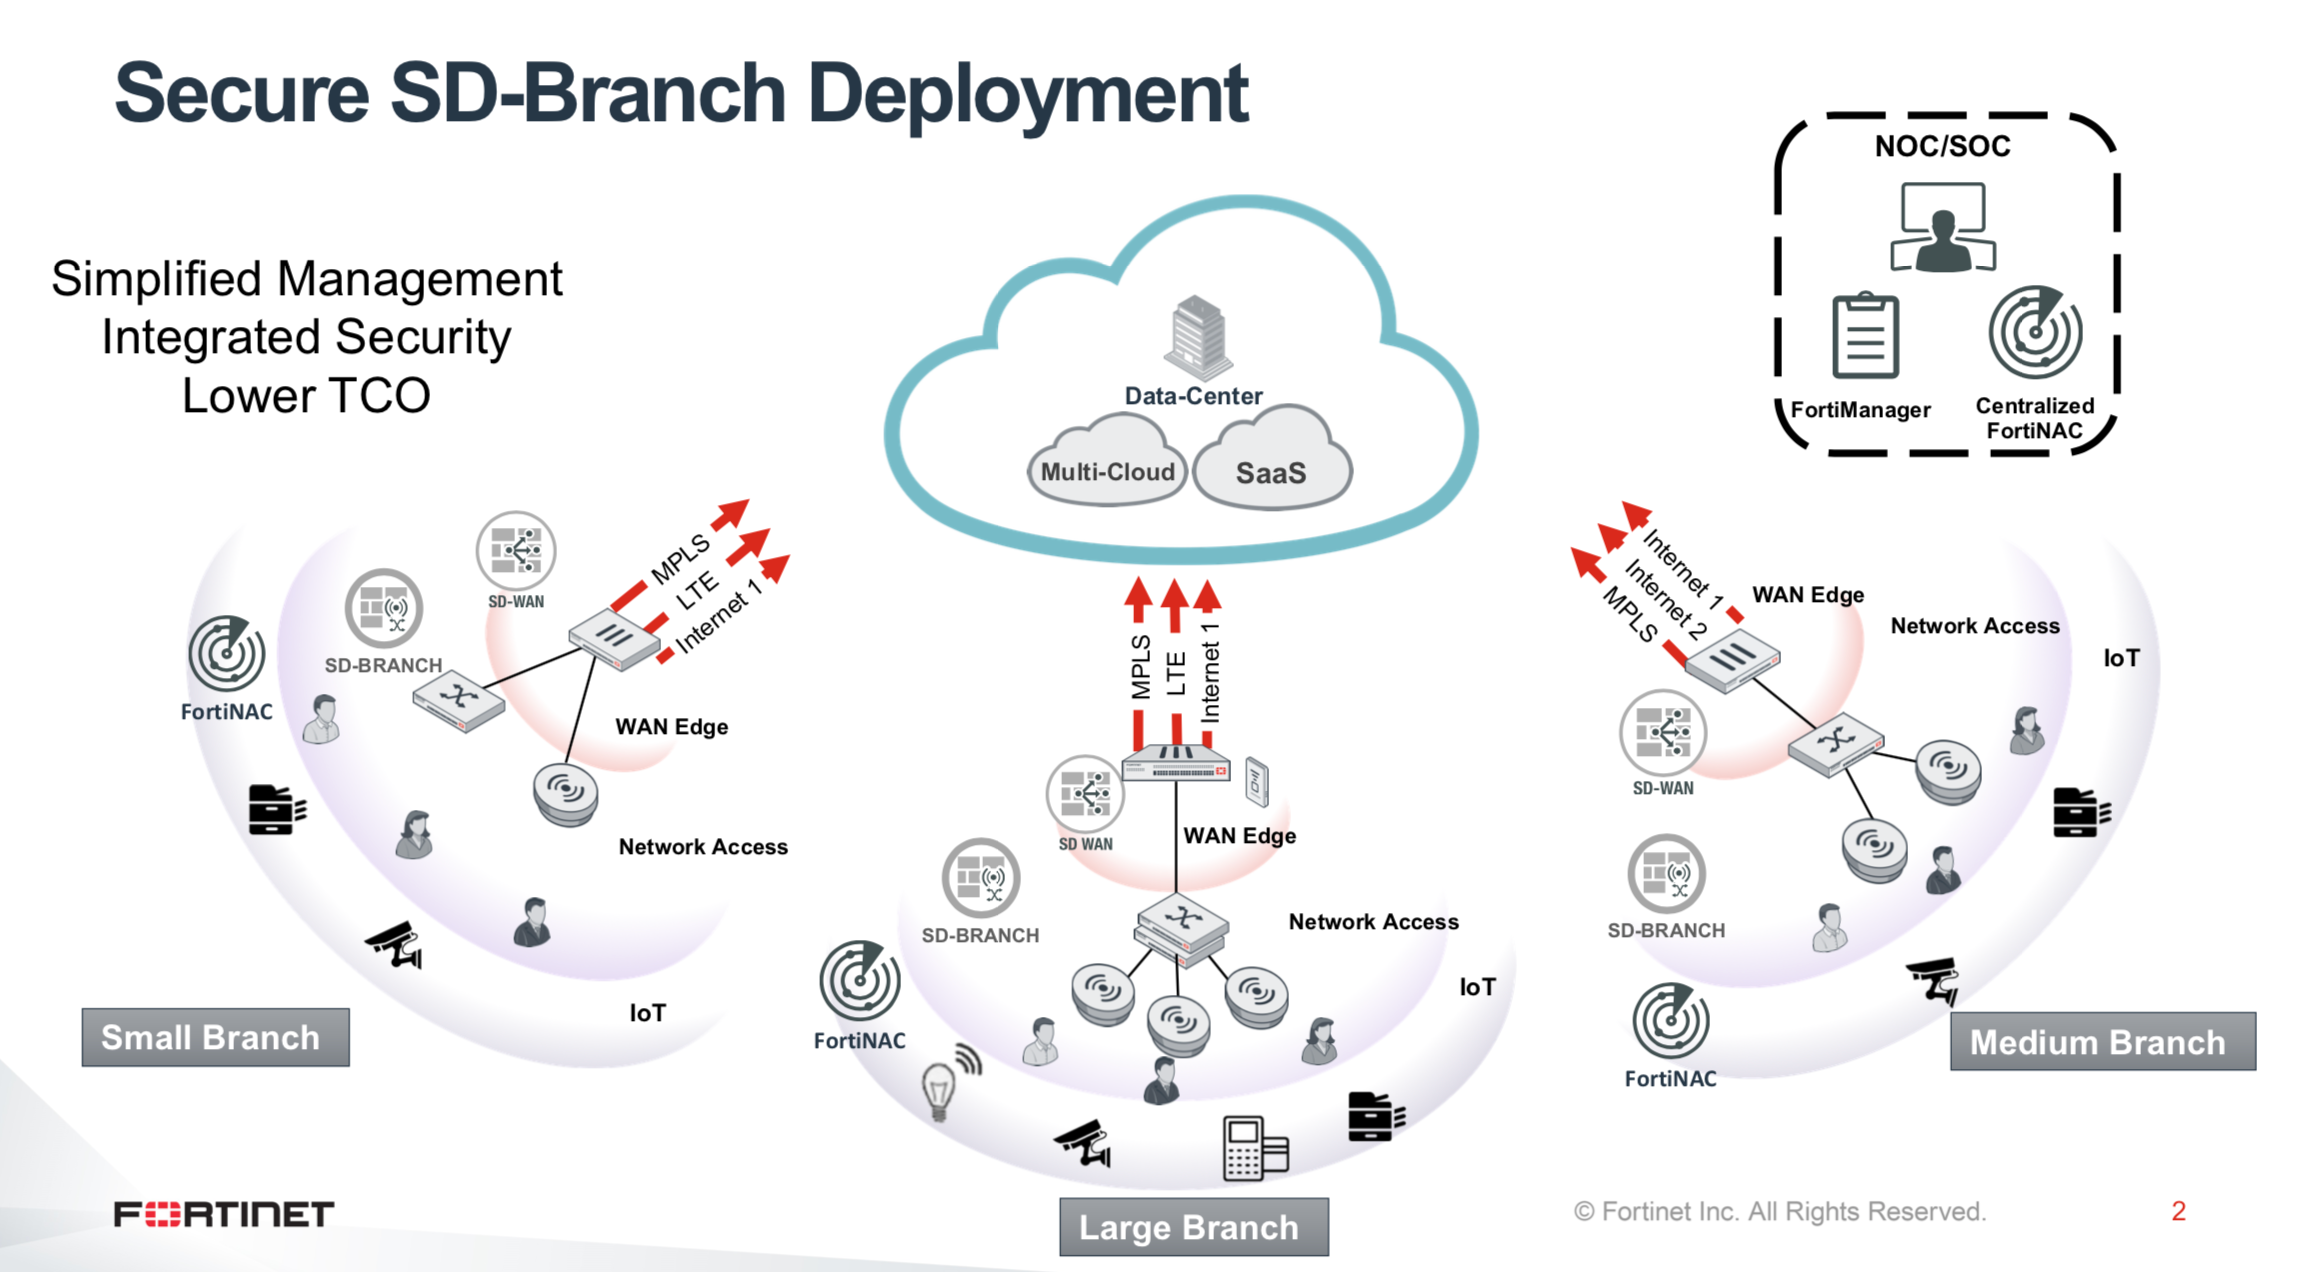
\includegraphics[width= 1\textwidth]{chapter1/sdwan fortinet.png}
    \caption{ SD-WAN by Fortinet\cite{ref9}}
    \label{fig:  SD-WAN by Fortinet}
\end{figure}
\subsection{Secure SD-WAN by Versa Networks}
Versa Networks’ SD-WAN solution offers a wide range of features designed to enhance network performance and reliability. It includes capabilities such as fast packet steering across multiple WAN interfaces, reduced packet loss, packet duplication, and the ability to bypass underperforming links. Additionally, it supports both encrypted and non-encrypted overlays using protocols like MPLS/GRE (Generic Routing Encapsulation) or VXLAN (Virtual eXtensible Local-Area Network), dynamic IPSec overlays, and direct internet access.

What sets Secure SD-WAN apart is its ability to integrate security, visibility, automation, and performance into a single platform. This comprehensive approach helps organizations tackle challenges and overcome complexities in their networks. With a unified graphical interface, Secure SD-WAN ensures rapid and scalable deployment while maintaining robust security. It also improves application performance, reduces the attack surface, and keeps implementation costs low.

Versa’s control plane is highly flexible, supporting all types of topologies and ensuring seamless setup for any tenant. Each tenant is assigned a single VRF (Virtual Routing and Forwarding) instance, which defines its specific topology. However, additional VRFs can be assigned to the same tenant, allowing them to participate in different topologies as needed\cite{ref10}.

\begin{figure}[H]
    \centering
    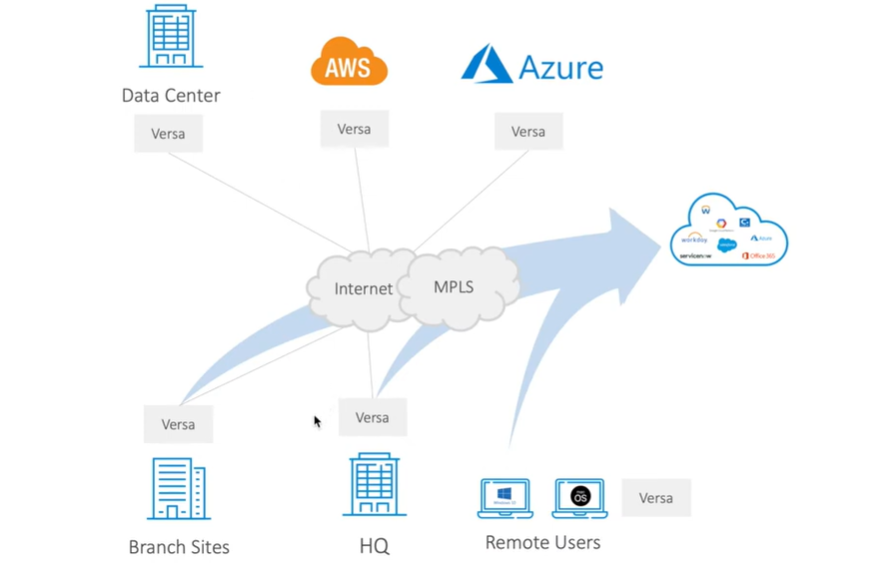
\includegraphics[width= 1\textwidth]{chapter1/sdwan versa.png}
    \caption{SD-WAN by Versa Networks\cite{ref10}}
    \label{fig:  SD-WAN by Versa Networks}
\end{figure}

\subsection{Cisco Viptela SD-WAN: Definition and Architecture}
On August 1, 2017, Cisco acquired Viptela, a San Jose-based startup renowned for its innovative SD-WAN solution. Today, Cisco offers two distinct SD-WAN options to cater to varying organizational needs:
        \begin{itemize}
            \item \textbf{Meraki :} A cloud-managed, plug-and-play solution designed for simplicity and ease of use, ideal for smaller networks or less complex environments\cite{ref12}.
            \item \textbf{Viptela :} A robust, enterprise-grade platform tailored for scalability and flexibility, particularly suited for large-scale deployments\cite{ref11}.
        \end{itemize}

One of the standout features of Cisco’s SD-WAN is its versatility. It can be deployed on physical hardware, virtualized environments, or public cloud platforms, allowing businesses to adopt a hybrid approach. This flexibility enables organizations to evolve their networks incrementally, integrating new technologies without overhauling existing infrastructure.
\subsubsection{Core Components of Cisco Viptela SD-WAN}
Cisco’s SD-WAN architecture is built around four foundational planes, each managed by a dedicated component:
        \begin{itemize}
            \item \textbf{Orchestration Plane (vBond) :} Acts as the “broker” responsible for securely onboarding SD-WAN routers into the network overlay. The overlay abstracts the underlying physical infrastructure, enabling distributed and virtualized networks to operate seamlessly on top of existing hardware.
            \item \textbf{Management Plane (vManage) :} Serves as the central hub for configuring, monitoring, and troubleshooting the entire SD-WAN infrastructure. It uses the NETCONF protocol, which simplifies remote device management, to communicate with edge routers via DTLS/TLS encryption.
            \item \textbf{Control Plane (vSmart) :} Defines the network topology, enforces routing policies, and determines optimal traffic paths. It uses Cisco’s proprietary Overlay Management Protocol (OMP) to exchange routing information across the network.
            \item \textbf{Data Plane (vEdge) :} Handles actual data transmission between sites, executing routing decisions made by the control plane. vEdge devices are deployed as physical or virtual appliances at branch offices, ensuring efficient and secure data transport\cite{ref13}.
        \end{itemize}
\begin{figure}[H]
    \centering
    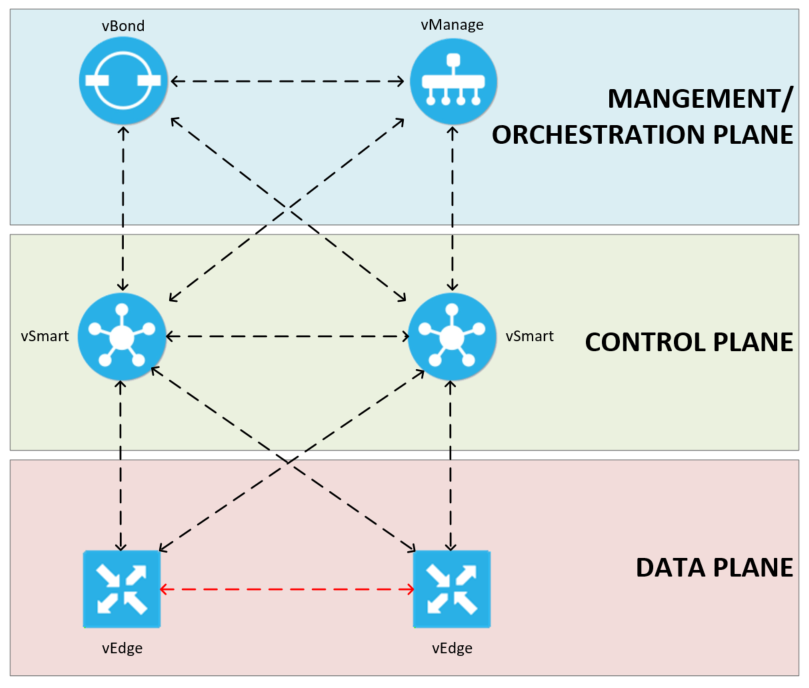
\includegraphics[width= 0.6\textwidth]{chapter1/SD-WAN planes.png}
    \caption{SD-WAN foundational planes\cite{ref14}}
    \label{fig: SD-WAN foundational planes}
\end{figure}
\subsubsection{How the Components Work Together}
The components of Cisco’s SD-WAN solution work in harmony to ensure seamless network operation:

vManage acts as the “brain” of the system, providing centralized configuration, monitoring, and enforcement of security policies.
vBond ensures secure and authenticated onboarding of new devices into the SD-WAN overlay network, maintaining a list of authorized components and facilitating communication between devices behind NATs.
vSmart dynamically calculates the most efficient paths for traffic based on real-time conditions, while vEdge devices execute these routing decisions to ensure optimal performance.
Protocols like OMP and NETCONF enable seamless communication between components, ensuring the network remains agile, secure, and responsive to changing demands\cite{ref4}.

The figure below illustrates this architecture :
\begin{figure}[H]
    \centering
    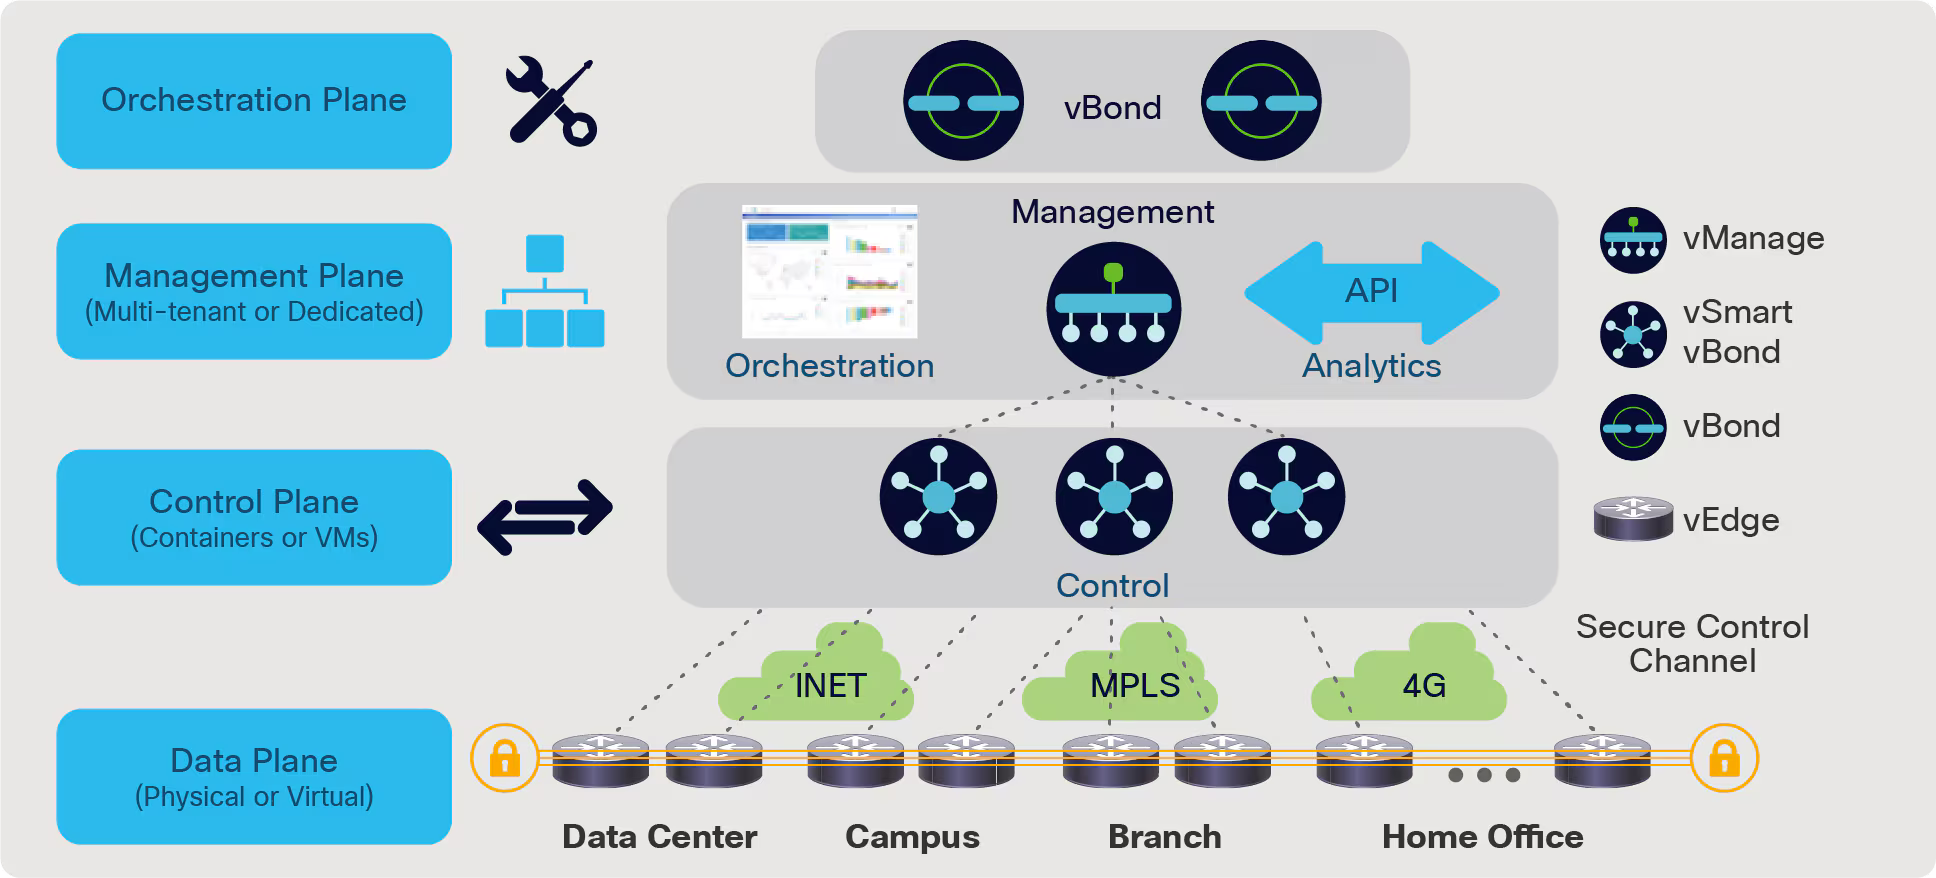
\includegraphics[width= 1\textwidth]{chapter1/sdwan cisco.png}
    \caption{Cisco’s SD-WAN solution\cite{ref15}}
    \label{fig: Cisco’s SD-WAN solution}
\end{figure}

\subsubsection{vBond: The SD-WAN Orchestrator}
vBond serves as the central orchestrator in Cisco’s SD-WAN infrastructure, automating critical tasks to ensure smooth operation of the Viptela solution. It links all software and hardware components, acting as the gateway for devices joining the SD-WAN overlay network.

vBond’s primary responsibilities include:

Authenticating devices to ensure only authorized components join the network.
Maintaining a registry of approved devices within the overlay.
Facilitating communication between devices located behind Network Address Translators (NATs) using a streamlined and secure mechanism.
By centralizing these functions, vBond enhances both the security and efficiency of the SD-WAN deployment process\cite{ref4}.
\subsubsection{vManage: The Central Control Hub}
vManage is the management server for Cisco’s SD-WAN solution, serving as the central control point for configuring, monitoring, and maintaining the network. It oversees the entire lifecycle of the SD-WAN deployment, broken into three key phases:
        \begin{itemize}
            \item \textbf{Day 0 (Design) :} Defining the network architecture, project requirements, and initial configurations.
            \item \textbf{Day 1 (Deployment) : }Rolling out the network design, setting up infrastructure, and deploying devices.
            \item \textbf{Day 2 (Maintenance) :} Managing ongoing operations, applying updates, and performing troubleshooting.
        \end{itemize}
vManage also provides comprehensive visibility into network performance, tracking metrics such as latency, bandwidth utilization, and packet loss. Additionally, it enforces security policies across the network, ensuring compliance and protecting against potential threats\cite{ref4}.
\subsubsection{OMP Protocol and Key Management}
Cisco’s proprietary Overlay Management Protocol (OMP) simplifies SD-WAN routing by centralizing updates through the vSmart controller. Key features of OMP include:
        \begin{itemize}
            \item \textbf{Key Management :} vSmart generates encryption keys for each router, reducing the processing burden on edge devices while maintaining robust security.
            \item \textbf{Routing Efficiency :} OMP functions similarly to BGP for internet routing but centralizes updates to prevent edge devices from being overwhelmed with excessive routing information.
            \item \textbf{Dynamic Updates :} Changes to network accessibility, gateway configurations, and security policies are managed centrally through vSmart, ensuring smoother performance and adaptability to evolving network conditions.
        \end{itemize}
This centralized approach enhances scalability and simplifies network management, making OMP a cornerstone of Cisco’s SD-WAN architecture\cite{ref4}.
\subsubsection{vEdge: The Flexible Edge Device}
vEdge devices form the backbone of Cisco’s SD-WAN solution, acting as the workhorses responsible for data transmission between sites. These devices are highly flexible, deployable as either physical hardware or virtual appliances, and can operate on-premises or in the cloud.
\textbf{Key characteristics of vEdge devices includes :}
\begin{enumerate}
    \item Supporting both physical and virtual deployments, enabling seamless integration into diverse environments.
    \item Executing routing decisions made by the control plane to ensure efficient and secure data transport.
    \item Providing robust performance and reliability, even in challenging network conditions.
    \item This flexibility makes vEdge devices an essential component of Cisco’s SD-WAN solution, capable of meeting the demands of modern enterprise networks.
\end{enumerate}
\begin{itemize}
    \item \textbf{Secure Data Flows} : Encrypt/decrypt traffic between SD-WAN sites.
    \item \textbf{Support Legacy Networks }: Work with standard protocols like BGP and OSPF.
    \item \textbf{Zero Touch Provisioning (ZTP)} : Automate setup, software updates, and configuration without manual intervention.
    \item \textbf{Monitoring and Alerts} : Send real-time events and security alerts to the management console\cite{ref4}.
\end{itemize}
\subsection{The Choice of Solution}
The table below provides a comparison of some proprietary solutions mentioned earlier. This comparative analysis highlights the strengths of the Cisco Viptela solution and explains why it was selected for implementation.
\begin{table}[h]
\centering
\footnotesize
\caption{Comparison Between Cisco Viptela, Fortinet, and Versa}
\label{tab:sdwan_comparison}
\begin{tabularx}{\linewidth}{@{}>{\raggedright\arraybackslash}p{2.8cm}>{\raggedright\arraybackslash}X>{\raggedright\arraybackslash}X>{\raggedright\arraybackslash}X@{}}
\toprule
\textbf{Feature} & \textbf{Cisco Viptela} & \textbf{Fortinet} & \textbf{Versa} \\
\midrule
\textbf{Network} 
& Supports both traditional routing and SD-WAN on single platform 
& Seamless migration with SD-WAN features 
& \makecell[l]{No infrastructure changes \\ Hardware additions needed} \\
\midrule
\textbf{Architecture} 
& \makecell[l]{Custom SD-WAN\\ Adaptable to business needs} 
& Legacy firewall-based 
& \makecell[l]{Dedicated components for:\\ - Control plane\\ - Data plane\\ - Management plane} \\
\midrule
\textbf{WAN Optimization} 
& TCP optimization + redundancy elimination 
& Limited optimization capabilities 
& Limited optimization capabilities \\
\midrule
\textbf{Security} 
& Full MPLS/VRF segmentation 
& Limited segmentation 
& Proven MPLS/VRF segmentation \\
\midrule
\textbf{Traffic Analysis} 
& Malware detection 
& \makecell[l]{Limited capability\\ Weak traffic analysis} 
& TLS/SSL encryption \\
\midrule
\textbf{Cloud} 
& Multi-cloud connectivity 
& \makecell[l]{Automated deployment\\ Multi-provider support} 
& \makecell[l]{Limited multi-cloud\\ Manual deployment} \\
\midrule
\textbf{Industrial Edge} 
& Ruggedized for harsh environments 
& Enhanced SD-WAN options 
& No enhanced options \\
\midrule
\textbf{Data Center} 
& Not supported 
& Not supported 
& Not supported \\
\bottomrule
\end{tabularx}
\end{table}

The Cisco Viptela solution was selected for implementation within the client’s network due to its numerous advantages. Its seamless migration process ensures a smooth transition without significant disruptions, while its adaptability allows for customization and scalability tailored to specific business needs. Additionally, Viptela offers simplified centralized management, enhanced visibility, and greater control through real-time monitoring tools, along with advanced security features such as data encryption. Furthermore, with intelligent traffic routing and optimization mechanisms, Viptela ensures optimal network performance, making it an ideal choice for modernizing and securing the client’s network.

\subsection{Certificates Used in Cisco Viptela SD-WAN}
The certification of controllers (vManage, vSmart, vBond) is essential for the successful implementation and operation of the Cisco Viptela solution. Two types of certificates are used in Cisco Viptela SD-WAN: controller certificates and web certificates\cite{ref16}.

\subsubsection{The Viptela Web Certificate}
The Viptela web certificate is designed to provide secure and private web access to vManage. Typically, Cisco installs a self-signed certificate, which is an SSL certificate signed by its creator rather than a trusted third-party Certificate Authority (CA). Cisco does not provide publicly issued web certificates from a CA. However, it recommends using their proprietary web server certificate in cases where enterprise networks may have firewalls with restricted web access policies. This ensures secure communication while adhering to organizational security requirements.
\subsubsection{The Viptela Controller Certificate}
The Viptela controller certificate is specifically designed to establish control connections between the controllers. These certificates are critical for the entire control plane of the Cisco Viptela SD-WAN solution and must be permanently stored. They play a vital role in securing communications across the SD-WAN infrastructure, ensuring that all control-plane interactions remain trusted and encrypted. Without these certificates, the integrity and functionality of the control plane would be compromised, underscoring their importance in maintaining a robust and secure SD-WAN environment\cite{ref16}.
\begin{figure}[H]
    \centering
    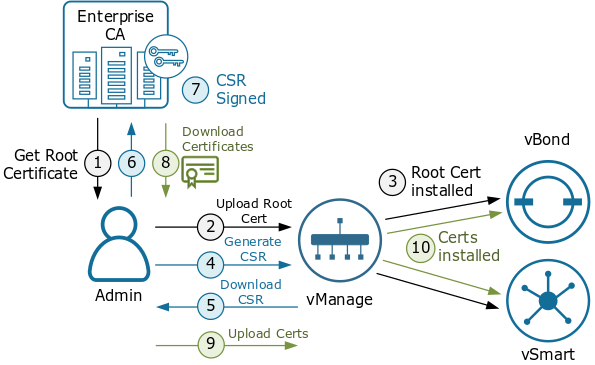
\includegraphics[width= 0.9\textwidth]{chapter1/certification.png}
    \caption{The Controller Certificate\cite{ref16}}
    \label{fig: The Controller Certificate}
\end{figure}
\section{Conclusion}
This chapter has established the rationale behind adopting SD-WAN within 3S and justified the decision to implement Cisco Viptela as the chosen solution. The limitations of legacy WAN architectures were clearly outlined, and the advantages of transitioning to a modern, software-defined network were emphasized.

Key components of the Cisco Viptela SD-WAN architecture (vBond, vManage, vSmart and vEdge) were explained, along with their roles in ensuring secure, scalable, and efficient network operations.

With the background, technical foundation, and vendor evaluation now complete, the next chapter will focus on the hands-on implementation of the selected solution, detailing the configuration steps, testing procedures, and deployment outcomes.

%%%%%%%%%%%%%%%%%%%%%%%%%%%%%%%%%%%%%%%%%%%%%%%%%%%%%%%%%%%%%%%%%%%%%%%%%%%%%%%%%%%%%%%%%%%%%%%%%%%%%%%%%%%%%%%%%%%%%%%%%%%%%%%%
\chapter{Implementation of Cisco SD-WAN – CLI Configuration}
\section{Introduction}
This chapter focuses on the initial phase of the Cisco Viptela SD-WAN implementation, specifically the device-level configuration using the command-line interface (CLI). It covers the setup of core components such as vBond, vSmart, and vEdge routers, along with detailed configurations for transport interfaces, routing protocols, and certificate-based authentication. These hands-on tasks form the technical backbone of the SD-WAN architecture before moving to centralized management.

\section{Architecture Overview}
The network is designed as a Hub and Spoke topology , where Site 300 serves as the central hub, connecting multiple distributed spokes (Sites 200, 400, and 500). Site 100 (HQ) is dedicated to hosting SD-WAN controllers (e.g., vManage, vSmart, vBond), which manage the entire network. The architecture leverages VRFs for traffic segmentation and uses MPLS for secure and efficient connectivity between the hub and spokes.

Hub : Site 300 acts as the central point of connectivity, managing traffic between all spokes.
Spokes : Sites 200, 400, and 500 are distributed locations connected to the hub via MPLS links.

SD-WAN Controllers : Site 100 hosts the SD-WAN management infrastructure, including controllers like vManage, vSmart, and vBond.
The network equipment utilized in the Cisco Viptela SD-WAN solution, including controllers, routers, and vEdge devices, is outlined in the table in appendix \texttt{(see appendix)}.
\afterpage{%
    \newgeometry{margin=0pt}
    \begin{figure}[p]
        \centering
        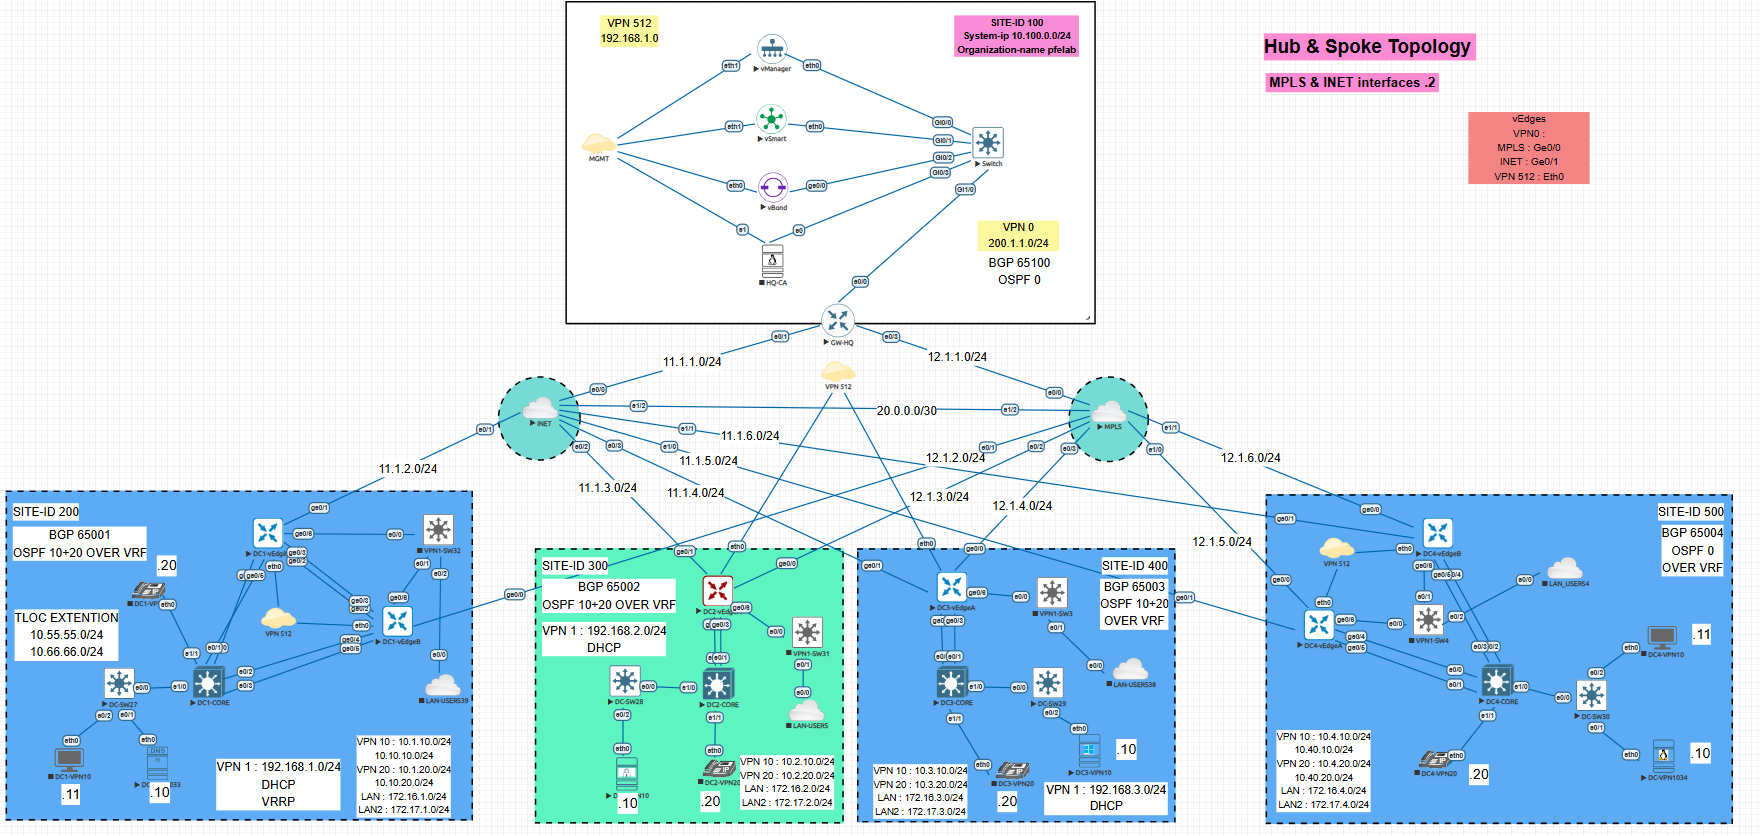
\includegraphics[
            width=0.9\paperheight,  % Swap width and height for rotation
            height=0.9\paperwidth,
            angle=270,
            origin=c
        ]{chapitre 3/new-topology.png}
        \caption{Cisco SD-WAN Full Architecture}
    \end{figure}
     \clearpage
}

% Fix for Page 20 footer

\clearpage % Ensure page break (if needed)
\thispagestyle{fancy}
\subsection{Central Cortex: vBond, vSmart and vManage in Concert}
The centralized network plays a crucial role in the overall architecture of our SD-WAN solution, enabling centralized management and efficient optimization of network traffic. 

Site 100 is dedicated to hosting the SD-WAN management infrastructure. Key details include:
\begin{enumerate}
    \item Controllers :
        \begin{itemize}
        \item\textbf{vManage :} Centralized management platform.
        \item\textbf{vSmart :} Policy enforcement controller.
        \item\textbf{vBond :} Certificate authority for device authentication.
        \end{itemize}
    \item Network Management :
        \begin{itemize}
            \item Manages all vEdges and local routers across the network.
            \item Ensures consistent policy enforcement and monitoring.
        \end{itemize}
    \item VPNs :
        \begin{itemize}
            \item \textbf{VPN 512 :}
            \begin{itemize}
                \item Used for management traffic.
                \item Dynamic IP address allocation.
            \end{itemize}
            \item \textbf{VPN 0  :}
            \begin{itemize}
                \item Used for management traffic.
                \item IP address range : 200.1.1.0/24
            \end{itemize}
        \end{itemize}
    \item Routing Protocols :
        Site 100 uses OSPF in outer-site routing.
\end{enumerate}
\subsubsection{Route Oracle: The vSmart Intelligence Engine}

% Use minipage to place the images side by side
\begin{figure}[H]
    \begin{minipage}[b]{0.48\textwidth} % Left image
        \centering
        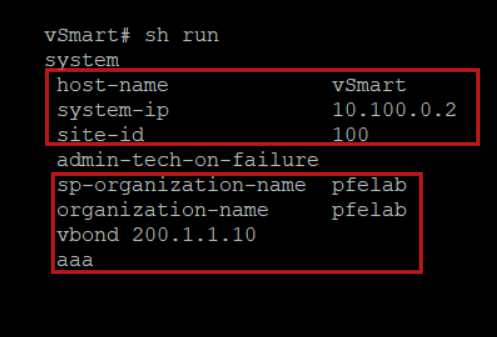
\includegraphics[width=\textwidth]{chapitre 3/21.png}
        \caption{vSmart System Configuration}
        \label{fig:vSmart System Configuration}
    \end{minipage}
    \hfill % Adds horizontal space between the two minipages
    \begin{minipage}[b]{0.48\textwidth} % Right image
        \centering
        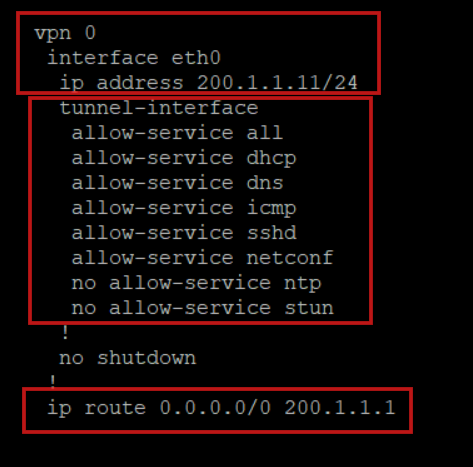
\includegraphics[width=\textwidth]{chapitre 3/22.png}
        \caption{vSmart Transport Configuration}
        \label{fig:vSmart Transport Configuration}
    \end{minipage}
\end{figure}

% Text and paragraphs go here, under both images
\textbf{vSmart Configuration Overview} \\
Basic settings of the vSmart controller, including host name, system IP, site ID, organization name, and vBond IP.

% At the very end of Page 20's content:
\vfill % Push next text to bottom
\hfill \textbf{\thepage} % Right-aligned page number
\renewcommand{\footrulewidth}{0.4pt} \footrule % Force rule

\newpage
\textbf{vSmart Transport Interface Configuration (VPN 0)} \\
Configuration of the transport interface (\texttt{eth0}) for general traffic forwarding, including allowed services and default route.

\textbf{vSmart Management Interface Configuration (VPN 512)} \\
    Configuration of the management interface (\texttt{eth1}) for network management, using DHCP for IP addressing.
\begin{figure}[H]
    \centering
    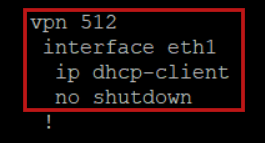
\includegraphics[width= 0.5\textwidth]{chapitre 3/23.png}
    \caption{vSmart Management Configuration}
    \label{fig: vSmart Management Configuration}
\end{figure}
\subsubsection{Trust Portal: The vBond Conduit}
- \textbf{vBond Configuration Overview} \\
    Basic settings of the vBond controller, including host name, system IP, site ID, organization name, and local vBond IP.
\begin{figure}[H]
    \centering
    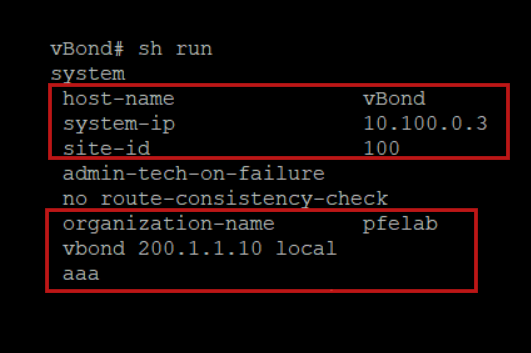
\includegraphics[width= 0.7\textwidth]{chapitre 3/24.png}
    \caption{vBond System Configuration}
    \label{fig: vBond System Configuration}
\end{figure}

% Use minipage to place the images side by side
\begin{figure}[H]
    \begin{minipage}[b]{0.48\textwidth} % Left image
        \centering
        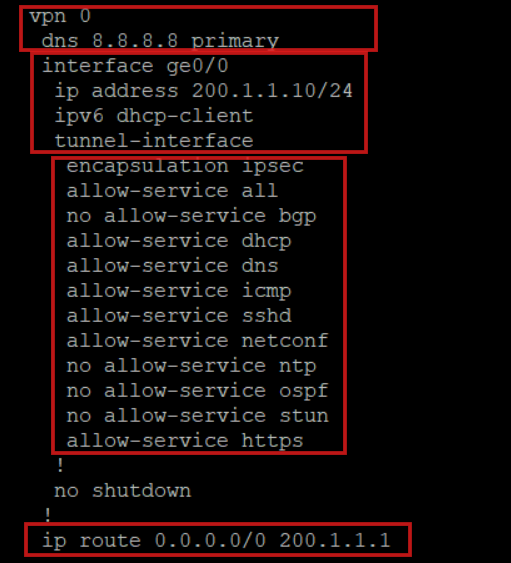
\includegraphics[width=\textwidth]{chapitre 3/25.png}
        \caption{vBond Transport Configuration}
        \label{fig:vBond Transport Configuration}
    \end{minipage}
    \hfill % Adds horizontal space between the two minipages
    \begin{minipage}[b]{0.48\textwidth} % Right image
        \centering
        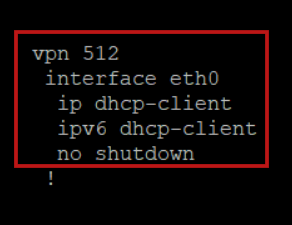
\includegraphics[width=\textwidth]{chapitre 3/26.png}
        \caption{vBond Management Configuration}
        \label{fig:vBond Management Configuration}
    \end{minipage}
\end{figure}
- \textbf{vBond Transport Interface Configuration (VPN 0)} \\
Configuration of the transport interface (\texttt{ge0/0}) for general traffic forwarding, including DNS, IP address, IPsec encapsulation, allowed services, and default route.

- \textbf{vBond Management Interface Configuration (VPN 512)} \\
Configuration of the management interface (\texttt{eth0}) for network management, using DHCP for IPv4 and IPv6 addressing.
\subsubsection{Policy Conductor: The vManage Command Deck}
\begin{figure}[H]
    \begin{minipage}[b]{0.6\textwidth} % Left image
        \centering
        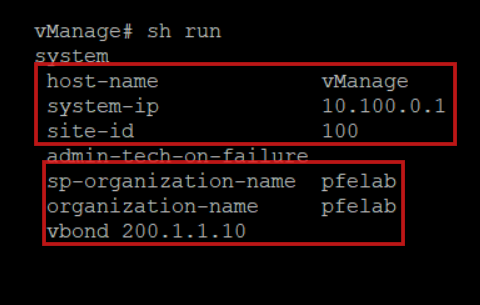
\includegraphics[width=\textwidth]{chapitre 3/18.png}
        \caption{vManage System Configuration}
        \label{fig:vManage System Configuration}
    \end{minipage}
    \hfill % Adds horizontal space between the two minipages
    \begin{minipage}[b]{0.30\textwidth} % Right image
        \centering
        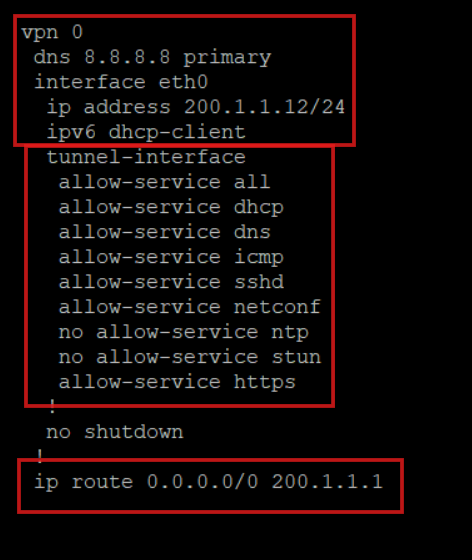
\includegraphics[width=\textwidth]{chapitre 3/19.png}
        \caption{vManage Transport Configuration}
        \label{fig:vManage Transport Configuration}
    \end{minipage}
\end{figure}
\textbf{vManage Configuration Overview} \\
Basic settings of the vManage controller, including host name, system IP, site ID, organization name, and vBond IP.

\textbf{vManage Transport Interface Configuration (VPN 0)} \\
Configuration of the transport interface (\texttt{eth0}) for general traffic forwarding, including DNS, IP address, allowed services, and default route.

\textbf{vManage Management Interface Configuration (VPN 512)} \\
    Configuration of the management interface (\texttt{eth1}) for network management, using DHCP for IP addressing.
\begin{figure}[H]
    \centering
    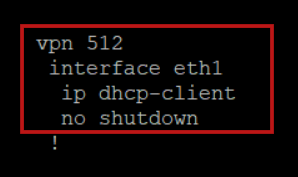
\includegraphics[width= 0.5\textwidth]{chapitre 3/20.png}
    \caption{vManage Management Configuration}
    \label{vManage Management Configuration}
\end{figure}
\section{Hub‑and‑Spoke Site Overview}
\subsection{Nexus Core (Central Hub – Site ID 300)}
Site 300 serves as the central hub and is depicted in the middle of the topology.
Key details include:
\begin{enumerate}
    \item \textbf{Core Router (vEdge):}
    \begin{itemize}
        \item Acts as the primary connection point for the hub.
        \item Interfaces:
        \begin{itemize}
            \item \textbf{MPLS (Ge0/0)}: Used for MPLS connectivity.
            \item \textbf{Internet (Ge0/1)}: Provides Internet access.
        \end{itemize}
        \item Overlay VPN membership:
        \begin{itemize}
            \item \textbf{VPN 512 (management)}: Used for network management.
            \item \textbf{VPN 0 (transport)}: Serves as the transport layer for general traffic.
        \end{itemize}
    \end{itemize}

    \item \textbf{Management Network (VPN 512):}
    \begin{itemize}
        \item Dedicated overlay for managing the network infrastructure.
        \item IP addresses are assigned dynamically via DHCP.
    \end{itemize}

    \item \textbf{Transport VPN (VPN 0):}
    \begin{itemize}
        \item Acts as the transport routing layer for general traffic.
        \item Underlay connections:
        \begin{itemize}
            \item \textbf{Internet:} \texttt{11.1.2.0/24}
            \item \textbf{MPLS:} \texttt{12.1.2.0/24}
        \end{itemize}
    \end{itemize}

    \item \textbf{Site‑Specific VPNs \& VRFs:}
    \begin{itemize}
        \item \textbf{VPN 1 (User LAN):} \texttt{192.168.2.0/24} with DHCP service and VRRP for gateway redundancy.
        \item \textbf{VPN 10 (Data‑Traffic):}
        \begin{itemize}
            \item Local prefix: \texttt{10.2.10.0/24}
            \item Exchanged with on‑site network \texttt{172.16.2.0/24}.
        \end{itemize}
        \item \textbf{VPN 20 (Voice‑Traffic):}
        \begin{itemize}
            \item Local prefix: \texttt{10.2.20.0/24}
            \item Exchanged with on‑site network \texttt{172.17.2.0/24}.
        \end{itemize}
    \end{itemize}

    \item \textbf{High Availability (HA) Components:}
    \begin{itemize}
        \item Redundant vEdge routers and VRRP ensure continuous service.
    \end{itemize}

    \item \textbf{Routing Protocols:}
    \begin{itemize}
        \item \textbf{BGP (AS 65002)}: Used for Internet‑side routing within VPN 0.
        \item \textbf{OSPF (Process ID 0)}: Used for MPLS‑side routing within VPN 0.
        \item \textbf{OSPF (Process IDs 10 \& 20 over VRF)}: Used for intra‑hub VRF exchange.
    \end{itemize}
\end{enumerate}
\subsubsection{DC2-vEdgeA Configuration Details}
\begin{enumerate}
    \item \textbf{vEdge Configuration Overview (Site 300)} \\
    Basic settings of the vEdge router (\texttt{dc2-vedgea}), including host name, system IP, site ID, organization name, and vBond IP.
\begin{figure}[H]
    \centering
    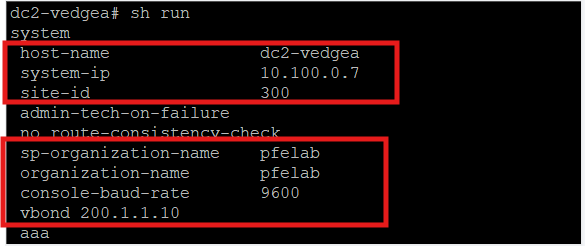
\includegraphics[width= 0.8\textwidth]{chapitre 3/2vedgea1.png}
    \caption{DC2-vEdgea System Configuration}
    \label{fig: DC2-vEdgea System Configuration}
\end{figure}
    \item \textbf{Tunnel Interface Configuration} \\
    Configures the tunnel interfaces (\texttt{ge0/0} and \texttt{ge0/1}) for secure communication, including IP addresses, IPsec encapsulation, and allowed services.
\begin{figure}[H]
    \centering
    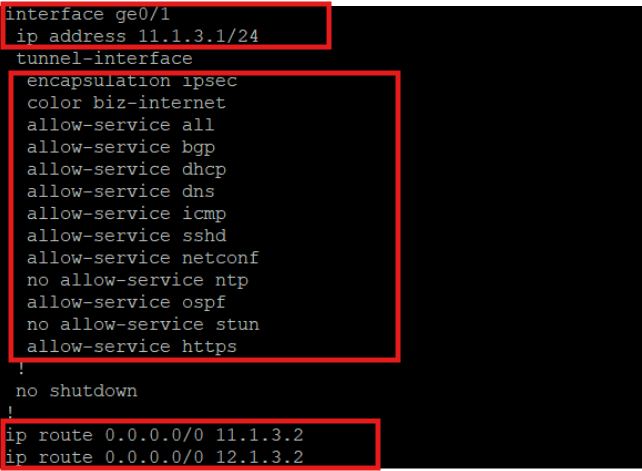
\includegraphics[width= 0.6\textwidth]{chapitre 3/2vedgea4.png}
    \caption{internet interface configuration}
    \label{fig: internet interface configuration}
\end{figure}
\begin{figure}[H]
    \centering
    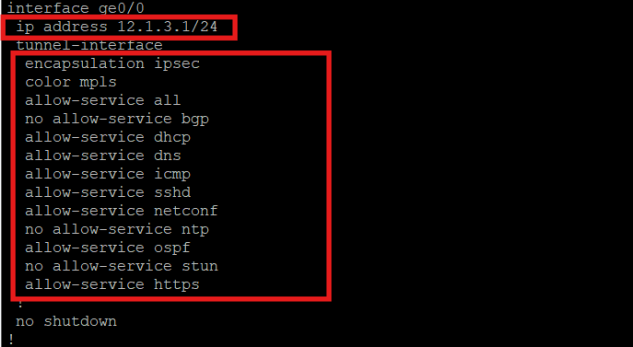
\includegraphics[width= 0.7\textwidth]{chapitre 3/2vedgea3.png}
    \caption{MPLS interface configuration}
    \label{fig: MPLS interface configuration}
\end{figure}
   

% Text and paragraphs go here, under both images
\item \textbf{Transport VPN routing Configuration} \\
Defines the transport VPN (\texttt{VPN 0}), including OSPF and BGP settings, tunnel interface configuration, and allowed services.

\item \textbf{Management Interface Configuration (VPN 512)} \\
Configures the management interface (\texttt{eth0}) for network management, using DHCP for IP addressing.
\end{enumerate}
\begin{figure}[H]
    \begin{minipage}[b]{0.48\textwidth} % Left image
        \centering
        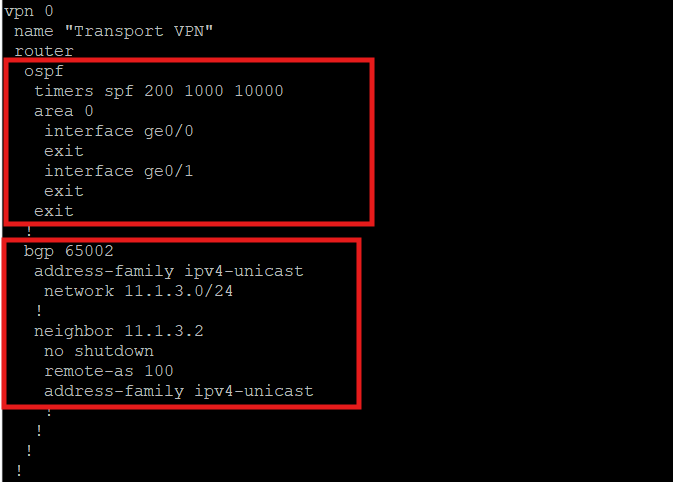
\includegraphics[width=\textwidth]{chapitre 3/2vedgea2.png}
        \caption{OSPF and BGP settings}
        \label{fig:OSPF and BGP settings}
    \end{minipage}
    \hfill % Adds horizontal space between the two minipages
    \begin{minipage}[b]{0.48\textwidth} % Right image
        \centering
        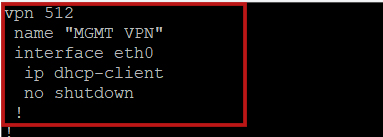
\includegraphics[width=\textwidth]{chapitre 3/dcvedge512.png}
        \caption{Management configuration}
        \label{fig:Management configuration}
    \end{minipage}
\end{figure}
\subsubsection{DC2-CORE router Configuration Details}
- \textbf{VRF Definition Configuration} \\
   This configuration defines two Virtual Routing and Forwarding (VRF) instances on the router (DC2-CORE), enabling logical segmentation of traffic.
\begin{figure}[H]
    \centering
    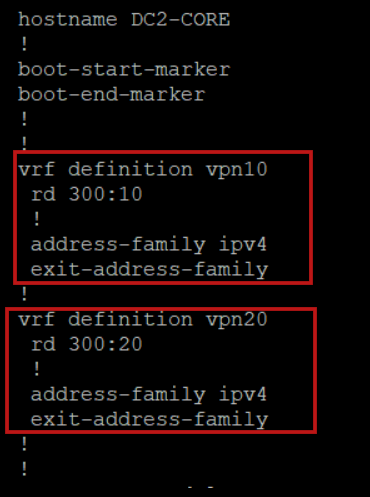
\includegraphics[width= 0.3\textwidth]{chapitre 3/9.png}
    \caption{VRF Definition Configuration}
    \label{fig: VRF Definition Configuration}
\end{figure}
- \textbf{Interface Configuration with VRF Assignment} \\
    This configuration assigns specific interfaces to the defined VRFs (vpn10 and vpn20) and configures IP addresses for each interface. 
- \textbf{OSPF Configuration for VRFs} \\
    This configuration enables OSPF routing within the defined VRFs (vpn10 and vpn20).
\begin{figure}[H]
    \centering
    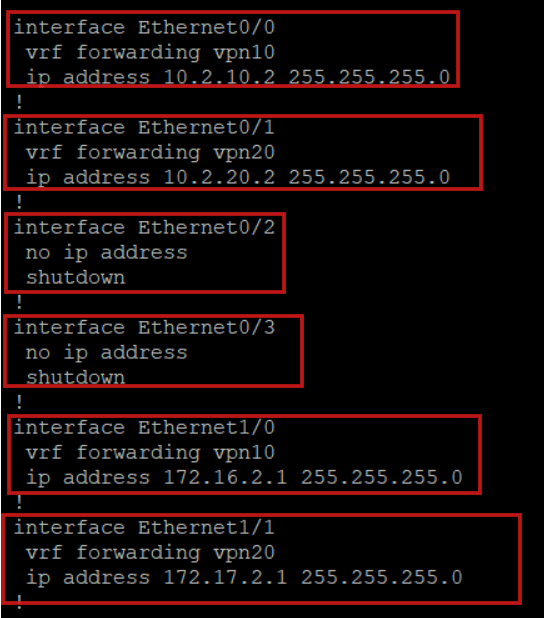
\includegraphics[width= 0.45\textwidth]{chapitre 3/10.png}
    \caption{Interface's VRF Assignment}
    \label{fig: Interface's VRF Assignment}
\end{figure}
- \textbf{Default Route Configuration for VRFs} \\
    This configuration sets default routes for each VRF (vpn10 and vpn20), specifying the next hop for traffic destined outside the local network.
\begin{figure}[H]
    \centering
    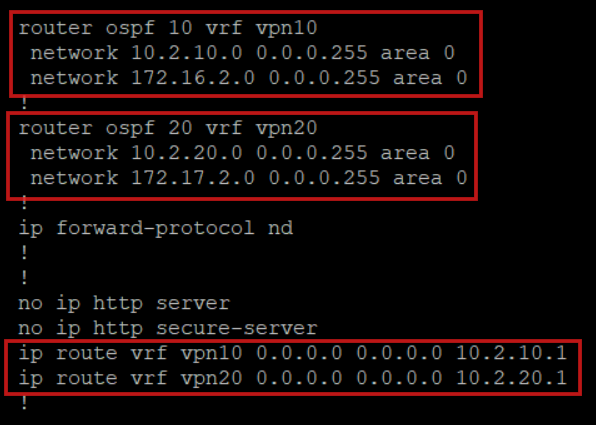
\includegraphics[width= 0.5\textwidth]{chapitre 3/11.png}
    \caption{VRFs Routing Configuration}
    \label{fig: VRFs Routing Configuration}
\end{figure}
\newpage
\subsection{Branch Spoke Sites (Sites 200, 400, 500)}
Each spoke site represents a remote branch connected to the central hub via MPLS (and Internet) underlays.  Key details include:

\begin{enumerate}
    \item \textbf{vEdge Routers:}
    \begin{itemize}
        \item Each site deploys one or more vEdge routers.
        \item Interfaces:
        \begin{itemize}
            \item \textbf{MPLS‐facing (Ge0/0)} for the private MPLS circuit to HQ.
            \item \textbf{Internet‐facing (Ge0/1)} for public Internet breakout.
        \end{itemize}
        \item Overlay VPN membership:
        \begin{itemize}
            \item \textbf{VPN 1} for user LAN (DHCP).
            \item \textbf{VPN 10} for DATA‑TRAFFIC.
            \item \textbf{VPN 20} for VOICE‑TRAFFIC.
        \end{itemize}
    \end{itemize}

    \item \textbf{Local Routers \& Switches:}
    \begin{itemize}
        \item Local core routers manage on‐site routing and peer with the vEdge via OSPF.
        \item Layer 2 switches provide LAN connectivity to end‑user devices.
    \end{itemize}

    \item \textbf{VRF Segmentation:}
    \begin{itemize}
        \item Each site uses VRFs to isolate traffic:
        \begin{itemize}
            \item \textbf{Site 200:} VRF 10 (DATA‑TRAFFIC), VRF 20 (VOICE‑TRAFFIC)
            \item \textbf{Site 400:} VRF 10 (DATA‑TRAFFIC), VRF 20 (VOICE‑TRAFFIC)
            \item \textbf{Site 500:} VRF 10 (DATA‑TRAFFIC), VRF 20 (VOICE‑TRAFFIC)
        \end{itemize}
        \item VRF routes are exchanged locally via OSPF and advertised into the SD‑WAN overlay by OMP.
    \end{itemize}

    \item \textbf{DHCP \& VRRP High Availability:}
    \begin{itemize}
        \item \textbf{VPN 1} serves as the DHCP scope for regular users at each spoke.
        \item Sites with dual vEdges employ \textbf{VRRP} on VPN 1 to present a single virtual gateway IP and ensure seamless fail‑over.
    \end{itemize}

\end{enumerate}

\subsection{Major Branch Office (Spoke – Site 200)}
\textbf{Location:} Large branch office.
Key configuration details include:
\begin{enumerate}
    \item \textbf{TLOC Extension:}
    \begin{itemize}
        \item Extends the transport overlay with additional subnets.
        \item Advertised networks: \texttt{10.55.55.0/24} and \texttt{10.66.66.0/24} for redundancy and load‑sharing across multiple transport paths.
    \end{itemize}

    \item \textbf{Transport VPN (VPN 0):}
    \begin{itemize}
        \item Serves as the transport routing layer for general traffic.
        \item Underlay connections:
        \begin{itemize}
            \item \textbf{Internet (11.1.2.0/24)} via \texttt{DC1‑vEdgeA}.
            \item \textbf{MPLS (12.1.2.0/24)} via \texttt{DC1‑vEdgeB}.
        \end{itemize}
    \end{itemize}

    \item \textbf{Management Network (VPN 512):}
    \begin{itemize}
        \item Dedicated overlay for device management.
        \item IP addresses assigned dynamically via DHCP.
    \end{itemize}

    \item \textbf{Site‑Specific VPNs \& VRFs:}
    \begin{itemize}
        \item \textbf{VPN 1 (User LAN):} \texttt{192.168.1.0/24} with DHCP service and VRRP for gateway redundancy.
        \item \textbf{VPN 10 (Data‑Traffic):}  
        \begin{itemize}
            \item Local prefixes: \texttt{10.1.10.0/24}, \texttt{10.10.10.0/24}  
            \item Exchanged with on‑site VRF network \texttt{172.16.1.0/24}.
        \end{itemize}
        \item \textbf{VPN 20 (Voice‑Traffic):}  
        \begin{itemize}
            \item Local prefixes: \texttt{10.1.20.0/24}, \texttt{10.10.20.0/24}  
            \item Exchanged with on‑site VRF network \texttt{172.17.1.0/24}.
        \end{itemize}
    \end{itemize}

    \item \textbf{Routing Protocols:}
    \begin{itemize}
        \item \textbf{BGP (AS 65001)} on \texttt{DC1‑vEdgeA} for Internet‑side routing within VPN 0.
        \item \textbf{OSPF (Process ID 0)} on \texttt{DC1‑vEdgeB} for MPLS‑side routing within VPN 0.
        \item \textbf{OSPF (Process IDs 10 \& 20 over VRF)} for on‑site VRF exchange.
    \end{itemize}
\end{enumerate}
\subsubsection{DC1-vEdgeA Configuration Details}
\begin{enumerate}
    \item \textbf{vEdge Configuration Overview (Site 200)} \\
    Basic settings of the vEdge router (\texttt{dcl-vedgea}), including host name, system IP, site ID, organization name, and vBond IP.

    \item \textbf{BGP Configuration for Transport VPN (VPN 0)} \\
    Defines BGP settings for the transport VPN, including AS number, network advertisement, and neighbor configuration.
\end{enumerate}
\begin{figure}[H]
    \begin{minipage}[b]{0.48\textwidth} % Left image
        \centering
        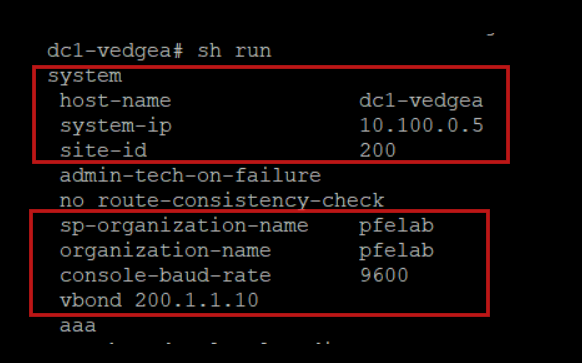
\includegraphics[width=\textwidth]{chapitre 3/27.png}
        \caption{DC1-vEdgea System Configuration}
        \label{fig:DC1-vEdgea System Configuration}
    \end{minipage}
    \hfill % Adds horizontal space between the two minipages
    \begin{minipage}[b]{0.48\textwidth} % Right image
        \centering
        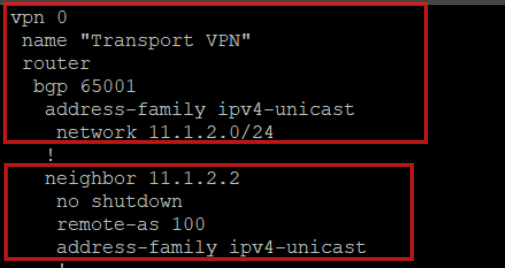
\includegraphics[width=\textwidth]{chapitre 3/28.1.png}
        \caption{BGP settings}
        \label{fig:BGP settings}
    \end{minipage}
\end{figure}  
    \item \textbf{Tunnel Interface Configuration} \\
    Configures the tunnel interface (\texttt{ge0/1}) for secure communication, including IP address, IPsec encapsulation, and allowed services.
\begin{figure}[H]
    \centering
    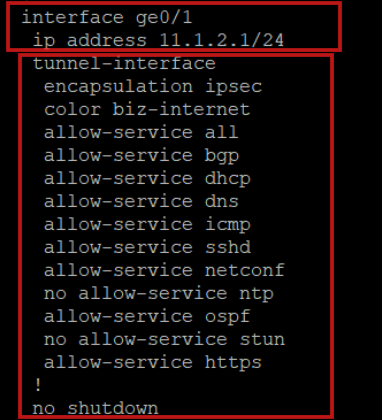
\includegraphics[width= 0.4\textwidth]{chapitre 3/28.2.png}
    \caption{Tunnel Interface Configuration}
    \label{fig: Tunnel Interface Configuration}
\end{figure}    
    \item \textbf{Management Interface Configuration (VPN 512)} \\
    Configures the management interface (\texttt{eth0}) for network management, using DHCP for IP addressing.
\begin{figure}[H]
    \centering
    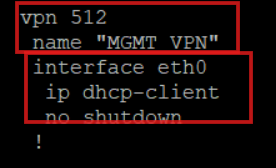
\includegraphics[width= 0.5\textwidth]{chapitre 3/29.png}
    \caption{Management Interface Configuration}
    \label{fig: Management Interface Configuration}
\end{figure}
\end{enumerate}
\subsubsection{DC1-vEdgeB Configuration Details}
\begin{enumerate}
    \item \textbf{vEdge Configuration Overview (Site 200)} \\
    Basic settings of the vEdge router (\texttt{dcl-vedgeb}), including host name, system IP, site ID, organization name, and vBond IP.
\begin{figure}[H]
    \centering
    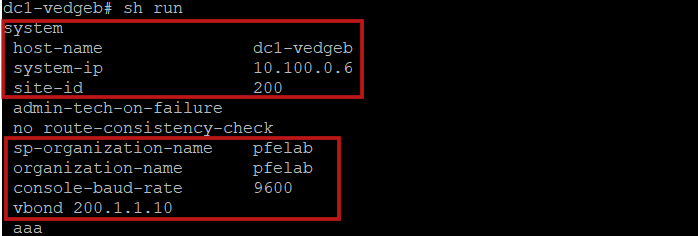
\includegraphics[width= 1\textwidth]{chapitre 3/dc1vedgeb1.png}
    \caption{DC1-vEdgeb System Configuration}
    \label{fig: DC1-vEdgeb System Configuration}
\end{figure}
    \item \textbf{Transport VPN (VPN 0) Configuration} \\
    Defines the transport VPN (\texttt{VPN 0}), including OSPF and BGP settings, tunnel interface configuration, and allowed services.
\begin{figure}[H]
    \centering
    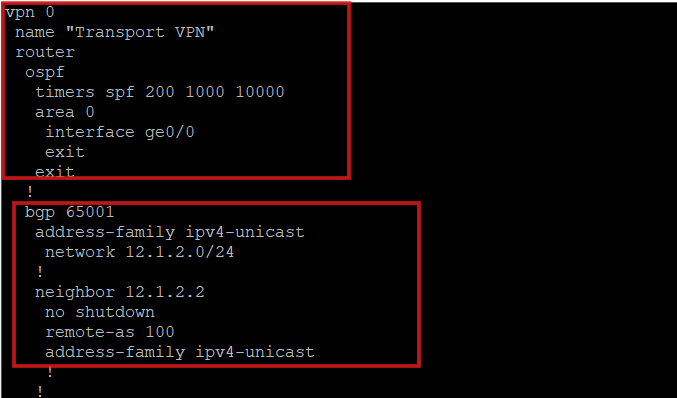
\includegraphics[width= 1\textwidth]{chapitre 3/dc1vedgeb2.png}
    \caption{OSPF and BGP settings}
    \label{fig: OSPF and BGP settings}
\end{figure}
\begin{figure}[H]
    \centering
    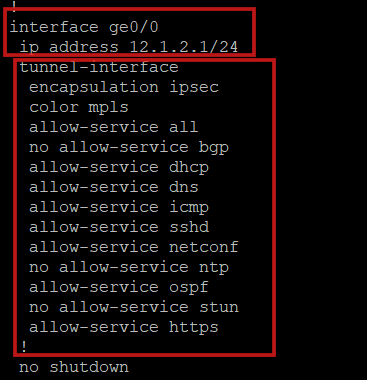
\includegraphics[width= 0.5\textwidth]{chapitre 3/dc1vedgeb3.png}
    \caption{Tunnel Configuration}
    \label{fig: Tunnel Configuration}
\end{figure}
    \item \textbf{Management VPN (VPN 512) Configuration} \\
    Defines the management VPN (\texttt{VPN 512}), including the interface (\texttt{eth0}) and DHCP client configuration.
\begin{figure}[H]
    \centering
    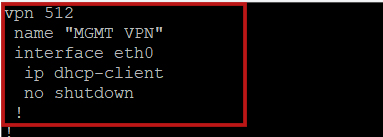
\includegraphics[width= 0.7\textwidth]{chapitre 3/dcvedge512.png}
    \caption{Management Interface Configuration}
    \label{fig: Management Interface Configuration}
\end{figure}
\end{enumerate}
\subsubsection{DC1-CORE}
\begin{enumerate}
    \item \textbf{VRF Definition Configuration} \\
    This configuration defines two Virtual Routing and Forwarding \texttt{(VRF)} instances on the router \texttt{(DC1-CORE)}, enabling logical segmentation of traffic.

    \item \textbf{Interface Configuration with VRF Assignment} \\
    This configuration assigns specific interfaces to the defined VRFs \texttt{(vpn10 and vpn20)} and configures IP addresses for each interface.
\end{enumerate}

% Use minipage to place the images side by side
\begin{figure}[H]
    \begin{minipage}[b]{0.48\textwidth} % Left image
        \centering
        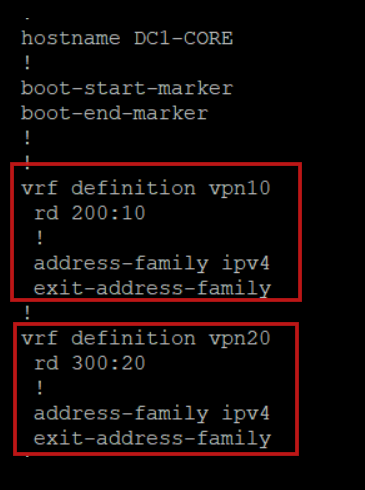
\includegraphics[width=\textwidth]{chapitre 3/6.png}
        \caption{DC1's VRF Definition}
        \label{fig:DC1's VRF Definition}
    \end{minipage}
    \hfill % Adds horizontal space between the two minipages
    \begin{minipage}[b]{0.48\textwidth} % Right image
        \centering
        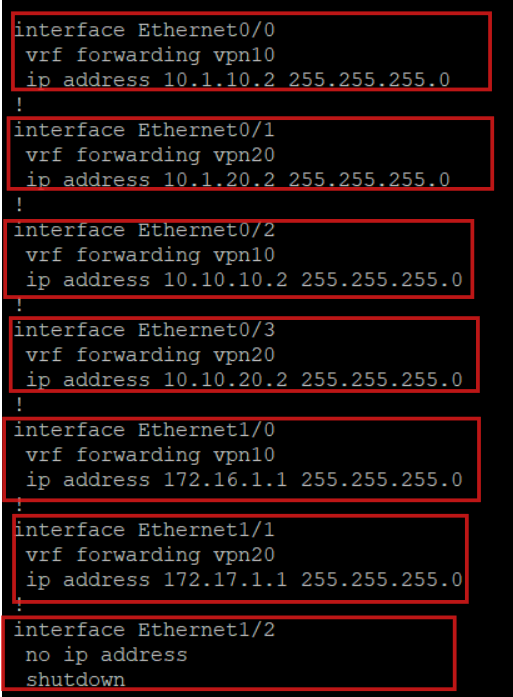
\includegraphics[width=\textwidth]{chapitre 3/7.png}
        \caption{DC1's VRF Assignment}
        \label{fig:DC1's VRF Assignment}
    \end{minipage}
\end{figure}
    \item \textbf{OSPF Configuration for VRFs} \\
   This configuration enables OSPF routing within the defined VRFs \texttt{(vpn10 and vpn20)}. 
    \item \textbf{Default Route Configuration for VRFs} \\
    This configuration sets default routes for each VRF \texttt{(vpn10 and vpn20)}, specifying the next hop for traffic destined outside the local network.
\begin{figure}[H]
    \centering
    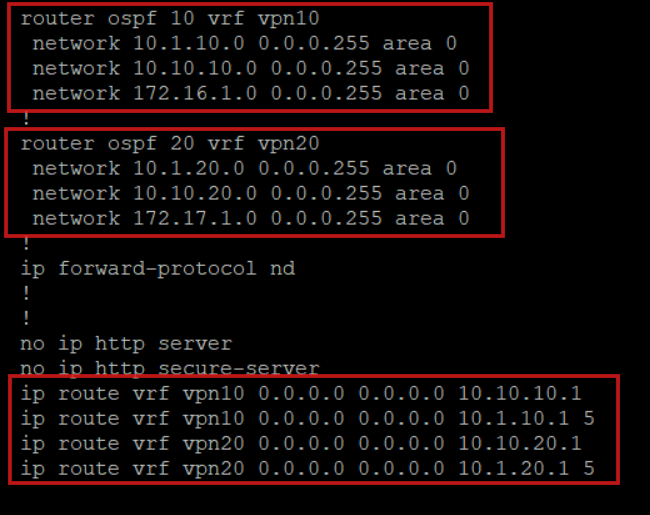
\includegraphics[width= 0.45\textwidth]{chapitre 3/8.png}
    \caption{VRFs Routing Configuration}
    \label{fig: VRFs Routing Configuration}
\end{figure}
\end{enumerate}
\subsection{Branch Office (Spoke – Site 400)}
\textbf{Location:} Branch office.
Key configuration details include:
\begin{enumerate}
    \item \textbf{Transport VPN (VPN 0):}
    \begin{itemize}
        \item Serves as the transport routing layer for general traffic.
        \item Underlay connections:
        \begin{itemize}
            \item \textbf{Internet:} \texttt{11.1.4.0/24} via \texttt{DC3‑vEdgeA}.
            \item \textbf{MPLS:} \texttt{12.1.4.0/24} via \texttt{DC3‑vEdgeB}.
        \end{itemize}
    \end{itemize}

    \item \textbf{Management Network (VPN 512):}
    \begin{itemize}
        \item Dedicated overlay for device management.
        \item IP addresses assigned dynamically via DHCP.
    \end{itemize}

    \item \textbf{Site‑Specific VPNs \& VRFs:}
    \begin{itemize}
        \item \textbf{VPN 1 (User LAN):} \texttt{192.168.3.0/24} with DHCP service.
        \item \textbf{VPN 10 (Data‑Traffic):}  
        \begin{itemize}
            \item Local prefix: \texttt{10.3.10.0/24}  
            \item Exchanged with on‑site VRF network \texttt{172.16.3.0/24}.
        \end{itemize}
        \item \textbf{VPN 20 (Voice‑Traffic):}  
        \begin{itemize}
            \item Local prefix: \texttt{10.3.20.0/24}  
            \item Exchanged with on‑site VRF network \texttt{172.17.3.0/24}.
        \end{itemize}
    \end{itemize}

    \item \textbf{Routing Protocols:}
    \begin{itemize}
        \item \textbf{BGP (AS 65003)} on \texttt{DC3‑vEdgeA} for Internet‑side routing within VPN 0.
        \item \textbf{OSPF (Process ID 0)} on \texttt{DC3‑vEdgeB} for MPLS‑side routing within VPN 0.
        \item \textbf{OSPF (Process IDs 10 \& 20 over VRF)} for on‑site VRF exchange.
    \end{itemize}
\end{enumerate}
\subsubsection{DC3-vEdgeA Configuration Details}
\begin{enumerate}
    \item \textbf{vEdge Configuration Overview (Site 400)} \\
    Basic settings of the vEdge router (\texttt{dc3-vedgea}), including host name, system IP, site ID, organization name, and vBond IP.
\begin{figure}[H]
    \centering
    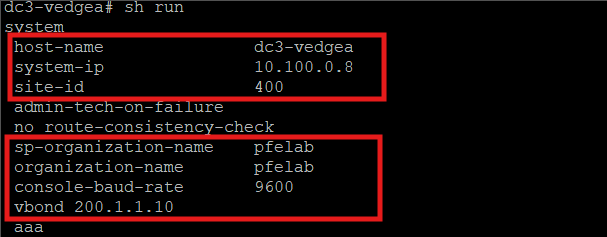
\includegraphics[width= 0.7\textwidth]{chapitre 3/3vedgea1.png}
    \caption{DC3-vEdgea System Configuration}
    \label{fig: DC3-vEdgea System Configuration}
\end{figure}
    \item \textbf{Tunnel Interface Configuration} \\
    Configures the tunnel interfaces (\texttt{ge0/0} and \texttt{ge0/1}) for secure communication, including IP addresses, IPsec encapsulation, and allowed services.
\begin{figure}[H]
    \centering
    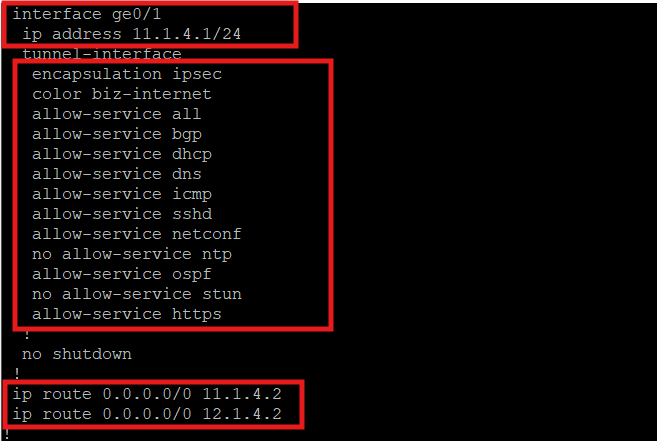
\includegraphics[width= 0.7\textwidth]{chapitre 3/3vedgea4.png}
    \caption{internet interface configuration}
    \label{fig: internet interface configuration}
\end{figure}
\begin{figure}[H]
    \centering
    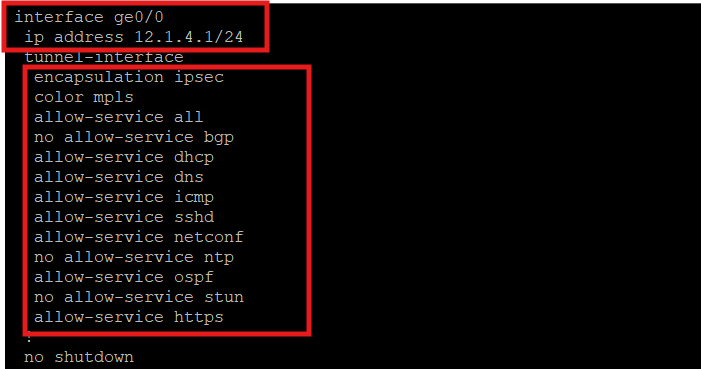
\includegraphics[width= 0.7\textwidth]{chapitre 3/3vedgea3.png}
    \caption{MPLS interface configuration}
    \label{fig: MPLS interface configuration}
\end{figure}
    \item \textbf{Transport VPN (VPN 0) Configuration} \\
    Defines the transport VPN (\texttt{VPN 0}), including OSPF and BGP settings, tunnel interface configuration, and allowed services.
\begin{figure}[H]
    \centering
    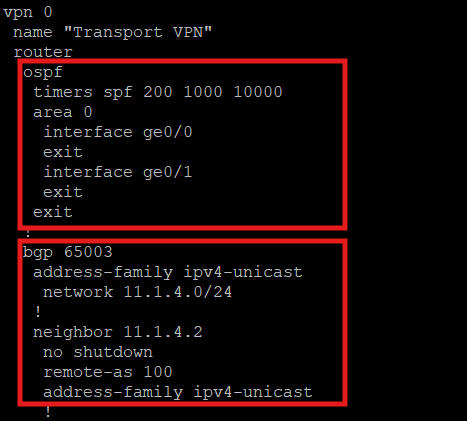
\includegraphics[width= 0.7\textwidth]{chapitre 3/3vedgea2.png}
    \caption{Site 400's OSPF and BGP settings}
    \label{fig: Site 400's OSPF and BGP settings}
\end{figure}
    \item \textbf{Management Interface Configuration (VPN 512)} \\
    Configures the management interface (\texttt{eth0}) for network management, using DHCP for IP addressing.
\begin{figure}[H]
    \centering
    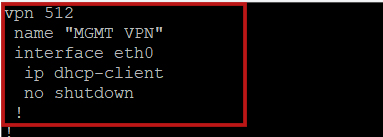
\includegraphics[width= 0.7\textwidth]{chapitre 3/dcvedge512.png}
    \caption{Management Configs}
    \label{fig: Management Configs}
\end{figure}
\end{enumerate}
\subsubsection{DC3-CORE Configuration Details}
\begin{enumerate}
    \item \textbf{VRF Definition Configuration} \\
    Defines two VRF instances (\texttt{vpn10} and \texttt{vpn20}) with route distinguishers and IPv4 addressing.

    \item \textbf{Interface Configuration with VRF Assignment} \\
    Assigns specific interfaces to the defined VRFs (\texttt{vpn10} and \texttt{vpn20}) and configures IP addresses for each interface.
\end{enumerate}

% Use minipage to place the images side by side
\begin{figure}[H]
    \begin{minipage}[b]{0.4\textwidth} % Left image
        \centering
        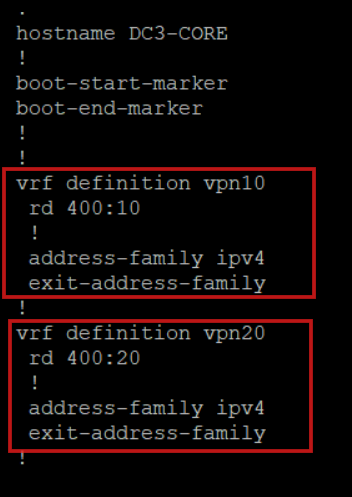
\includegraphics[width=\textwidth]{chapitre 3/12.png}
        \caption{DC3's VRF Definition}
        \label{fig:DC3's VRF Definition}
    \end{minipage}
    \hfill % Adds horizontal space between the two minipages
    \begin{minipage}[b]{0.48\textwidth} % Right image
        \centering
        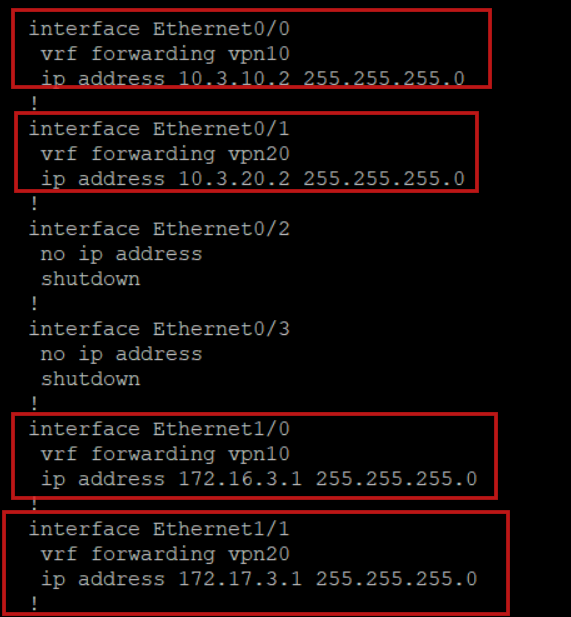
\includegraphics[width=\textwidth]{chapitre 3/13.png}
        \caption{DC3's VRF Assignment}
        \label{fig:DC3's VRF Assignment}
    \end{minipage}
\end{figure}
    \item \textbf{OSPF Configuration for VRFs} \\
    Enables OSPF routing within each VRF (\texttt{vpn10} and \texttt{vpn20}) using separate OSPF process IDs and network statements.
\begin{figure}[H]
    \centering
    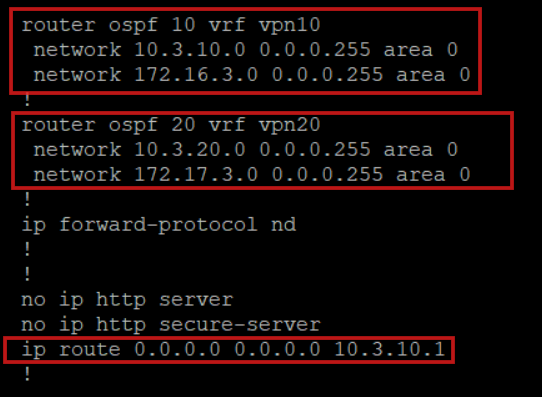
\includegraphics[width= 0.5\textwidth]{chapitre 3/14.png}
    \caption{DC3 VRFs Routing Configuration}
    \label{fig: DC3 VRFs Routing Configuration}
\end{figure}    
    \item \textbf{Default Route Configuration} \\
    Sets a default route for general traffic forwarding.
\end{enumerate}
\subsection{Major Branch Office (Spoke – Site 500)}
\textbf{Location:} Large branch office.
Key configuration details include:
\begin{enumerate}
    \item \textbf{Transport VPN (VPN 0):}
    \begin{itemize}
        \item Serves as the transport routing layer for general traffic.
        \item Underlay connections:
        \begin{itemize}
            \item \textbf{Internet:} \texttt{11.1.5.0/24} via \texttt{DC5‑vEdgeA} and \texttt{11.1.6.0/24} via \texttt{DC5‑vEdgeB}.
            \item \textbf{MPLS:} \texttt{12.1.5.0/24} via \texttt{DC5‑vEdgeA} and \texttt{12.1.6.0/24} via \texttt{DC5‑vEdgeB}.
        \end{itemize}
    \end{itemize}

    \item \textbf{Management Network (VPN 512):}
    \begin{itemize}
        \item Dedicated overlay for device management.
        \item IP addresses assigned dynamically via DHCP.
    \end{itemize}

    \item \textbf{Site‑Specific VPNs \& VRFs:}
    \begin{itemize}
        \item \textbf{VPN 1 (User LAN):} \texttt{192.168.4.0/24} with DHCP service and VRRP for gateway redundancy.
        \item \textbf{VPN 10 (Data‑Traffic):}  
        \begin{itemize}
            \item Local prefixes: \texttt{10.4.10.0/24}, \texttt{10.40.10.0/24}  
            \item Exchanged with on‑site VRF network \texttt{172.16.4.0/24}.
        \end{itemize}
        \item \textbf{VPN 20 (Voice‑Traffic):}  
        \begin{itemize}
            \item Local prefixes: \texttt{10.4.20.0/24}, \texttt{10.40.20.0/24}  
            \item Exchanged with on‑site VRF network \texttt{172.17.4.0/24}.
        \end{itemize}
    \end{itemize}

    \item \textbf{Routing Protocols:}
    \begin{itemize}
        \item \textbf{BGP (AS 65004)} on both \texttt{DC5‑vEdgeA} and \texttt{DC5‑vEdgeB} for Internet‑side routing within VPN 0.
        \item \textbf{OSPF (Process ID 0)} on both \texttt{DC5‑vEdgeA} and \texttt{DC5‑vEdgeB} for MPLS‑side routing within VPN 0.
        \item \textbf{OSPF (Process IDs 10 \& 20 over VRF)} for on‑site VRF exchange.
    \end{itemize}
\end{enumerate}
\subsubsection{DC4-vEdgeA Configuration Details}

\begin{enumerate}
    \item \textbf{vEdge Configuration Overview (Site 500)} \\
    Basic settings of the vEdge router (\texttt{dc4-vedgea}), including host name, system IP, site ID, organization name, and vBond IP.
\begin{figure}[H]
    \centering
    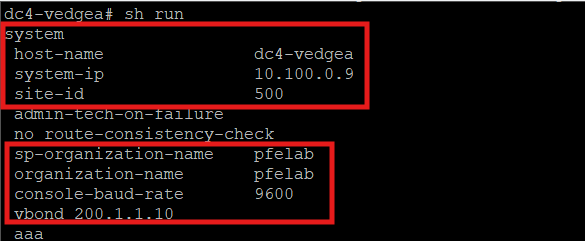
\includegraphics[width= 0.6\textwidth]{chapitre 3/4vedgea1.png}
    \caption{DC4-vEdgea System Configuration}
    \label{fig: Credentials Extraction}
\end{figure} 
    \item \textbf{Tunnel Interface Configuration} \\
    Configures the tunnel interfaces (\texttt{ge0/0} and \texttt{ge0/1}) for secure communication, including IP addresses, IPsec encapsulation, and allowed services.
\begin{figure}[H]
    \centering
    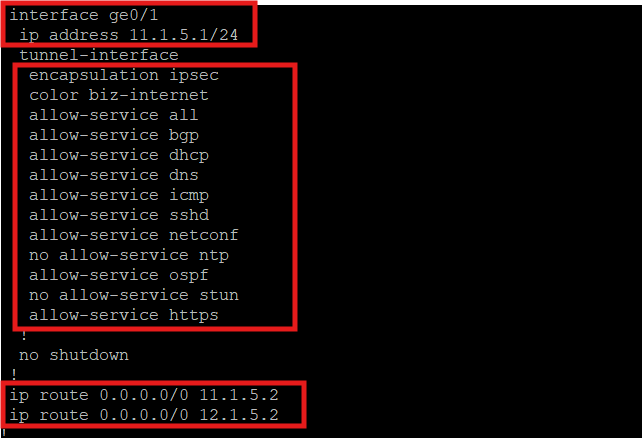
\includegraphics[width= 0.6\textwidth]{chapitre 3/4vedgea4.png}
    \caption{DC4-vEdgea's internet interface configuration}
    \label{fig: DC4 internet interface configuration}
\end{figure}
\begin{figure}[H]
    \centering
    \includegraphics[width= 0.75\textwidth]{chapitre 3/4vedgea3.png}
    \caption{DC4-vEdgea's MPLS interface configuration}
    \label{fig: DC4 MPLS interface configuration}
\end{figure}
    \item \textbf{Transport VPN (VPN 0) Configuration} \\
    Defines the transport VPN (\texttt{VPN 0}), including OSPF and BGP settings, tunnel interface configuration, and allowed services.
\begin{figure}[H]
    \centering
    \includegraphics[width= 0.7\textwidth]{chapitre 3/4vedgea2.png}
    \caption{DC4-vEdgea's  OSPF and BGP settings}
    \label{fig: DC4-vEdgea's OSPF and BGP settings}
\end{figure}
    \item \textbf{Management VPN (VPN 512) Configuration} \\
    Defines the management VPN (\texttt{VPN 512}), including the interface (\texttt{eth0}) and DHCP client configuration.
\begin{figure}[H]
    \centering
    \includegraphics[width= 0.7\textwidth]{chapitre 3/dcvedge512.png}
    \caption{DC4-vEdgea's Management Configs}
    \label{fig: DC4-vEdgea's Management Configs}
\end{figure}
\end{enumerate}
\subsubsection{DC4-vEdgeB Configuration Details}
\begin{enumerate}
    \item \textbf{vEdge Configuration Overview (Site 500)} \\
    Basic settings of the vEdge router (\texttt{dc4-vedgeb}), including host name, system IP, site ID, organization name, and vBond IP.
\begin{figure}[H]
    \centering
    \includegraphics[width= 0.8\textwidth]{chapitre 3/4vedgeb1.png}
    \caption{DC4-vEdgeb System Configuration}
    \label{fig: DC4-vEdgeb System Configuration}
\end{figure}    
    \item \textbf{Transport VPN (VPN 0) Configuration} \\
    Defines the transport VPN (\texttt{VPN 0}), including OSPF and BGP settings, tunnel interface configuration, and allowed services.
\begin{figure}[H]
    \centering
    \includegraphics[width= 0.8\textwidth]{chapitre 3/4vedgeb2.png}
    \caption{DC4-vEdgeb's OSPF and BGP settings}
    \label{fig: DC4-vEdgea's OSPF and BGP settings}
\end{figure}    
    \item \textbf{Tunnel Interface Configuration} \\
    Configures the tunnel interfaces (\texttt{ge0/0} and \texttt{ge0/1}) for secure communication, including IP addresses, IPsec encapsulation, and allowed services.
\begin{figure}[H]
    \centering
    \includegraphics[width= 0.75\textwidth]{chapitre 3/4vedgeb3.png}
    \caption{DC4-vEdgeb's MPLS interface configuration}
    \label{fig: DC4-vEdgeb's MPLS interface configuration}
\end{figure}
\begin{figure}[H]
    \centering
    \includegraphics[width= 0.7\textwidth]{chapitre 3/4vedgeb4.png}
    \caption{DC4-vEdgeb's internet interface configuration}
    \label{fig: DC4-vEdgeb's internet interface configuration}
\end{figure}
    \item \textbf{Management VPN (VPN 512) Configuration} \\
    Defines the management VPN (\texttt{VPN 512}), including the interface (\texttt{eth0}) and DHCP client configuration.
\end{enumerate}
\begin{figure}[H]
    \centering
    \includegraphics[width= 0.5\textwidth]{chapitre 3/dcvedge512.png}
    \caption{DC4-vEdgeb's Management Configs}
    \label{fig: DC4-vEdgeb's Management Configs}
\end{figure}
\subsubsection{DC4-CORE Configuration Details}
\begin{enumerate}
    \item \textbf{VRF Definition Configuration} \\
    Defines two VRF instances (\texttt{vpn10} and \texttt{vpn20}) with route distinguishers and IPv4 addressing.

    \item \textbf{Interface Configuration with VRF Assignment} \\
    Assigns specific interfaces to the defined VRFs (\texttt{vpn10} and \texttt{vpn20}) and configures IP addresses for each interface.
\end{enumerate}

% Use minipage to place the images side by side
\begin{figure}[H]
    \begin{minipage}[b]{0.48\textwidth} % Left image
        \centering
        \includegraphics[width=\textwidth]{chapitre 3/15.png}
        \caption{DC4's VRF Definition}
        \label{fig:DC4's VRF Definition}
    \end{minipage}
    \hfill % Adds horizontal space between the two minipages
    \begin{minipage}[b]{0.48\textwidth} % Right image
        \centering
        \includegraphics[width=\textwidth]{chapitre 3/16.png}
        \caption{DC4's VRF Assignment}
        \label{fig:DC4's VRF Assignment}
    \end{minipage}
\end{figure}
    \item \textbf{OSPF Configuration for VRFs} \\
    Enables OSPF routing within each VRF (\texttt{vpn10} and \texttt{vpn20}) using separate OSPF process IDs and network statements.
    \item \textbf{Default Route Configuration for VRFs} \\
    Sets default routes for each VRF, specifying the next hop for traffic destined outside the local network.
\begin{figure}[H]
    \centering
    \includegraphics[width= 0.8\textwidth]{chapitre 3/17.png}
    \caption{DC4 VRFs Routing Configuration}
    \label{fig: DC4 VRFs Routing Configuration}
\end{figure}    
\end{enumerate}
\subsection{Transport Layer Backbone: MPLS, Internet, and Central Gateway Integration}
This subsection provides an overview of the key network components in the SD-WAN architecture, including the MPLS Router, Internet (Inet) Router, and Headquarters Gateway (HQ-GW).The configurations detailed below highlight how these routers are configured to support VRFs, routing protocols (OSPF and BGP), interface settings, and default routes to facilitate seamless communication across the network.
\subsubsection{HQ-GW Configuration Details}
\begin{enumerate}
    \item \textbf{Interface Configuration} \\
    Configures the IP addresses for the HQ-GW interfaces (\texttt{Ethernet0/0}, \texttt{Ethernet0/1}, \texttt{Ethernet0/2}, \texttt{Ethernet0/3}).   
    \item \textbf{OSPF Configuration} \\
    Defines OSPF routing with specific network advertisements and passive/non-passive interface configurations.    
    \item \textbf{Default Route Configuration} \\
    Sets a default route for general traffic forwarding.
\end{enumerate}
\begin{figure}[H]
    \centering
    \includegraphics[width= 0.55\textwidth]{chapitre 3/1.png}
    \caption{HQ-GW Configuration}
    \label{fig: HQ-GW Configuration}
\end{figure}
\subsubsection{Internet router Configuration Details}
\begin{enumerate}
    \item \textbf{Interface Configuration for Internet Connectivity} \\
    Assigns static IP addresses to interfaces used for internet connectivity.
\begin{figure}[H]
    \centering
    \includegraphics[width= 0.35\textwidth]{chapitre 3/2.png}
    \caption{INET interface Configuration}
    \label{fig: INET interface Configuration}
\end{figure}
    \item \textbf{BGP Configuration for Internet Connectivity} \\
    Defines BGP settings, including AS number, router ID, neighbors, and advertised networks.
    \item \textbf{Default Route Configuration} \\
    Sets a default route for general traffic forwarding.
\begin{figure}[H]
    \centering
    \includegraphics[width= 0.4\textwidth]{chapitre 3/3.png}
    \caption{Inet Routing Configs}
    \label{fig: Inet Routing Configs}
\end{figure}
\end{enumerate}     

\subsubsection{MPLS router Configuration Details}
\begin{enumerate}
    \item \textbf{Interface Configuration for OSPF and BGP} \\
    Assigns static IP addresses and configures OSPF point-to-point settings for the interfaces.
\begin{figure}[H]
    \centering
    \includegraphics[width= 0.35\textwidth]{chapitre 3/4.png}
    \caption{MPLS interface Configuration}
    \label{fig: MPLS interface Configuration}
\end{figure}
    \item \textbf{OSPF and BGP Configuration for Routing} \\
    Defines OSPF and BGP settings to ensure seamless routing and interconnectivity between networks.
\begin{figure}[H]
    \centering
    \includegraphics[width= 0.45\textwidth]{chapitre 3/5.png}
    \caption{MPLS Routing Configs}
    \label{fig: MPLS Routing Configs}
\end{figure}
\end{enumerate}
\section{Building Trust in SD-WAN: The Role of Certificates}
Setting up certificates for SD-WAN components like vSmart, vManage, vBond and the vedges is an essential part of building a secure and trustworthy Cisco SD-WAN network. These certificates allow the different parts of the system to recognize each other and communicate over encrypted channels, creating a secure control plane. Normally, certificates are installed during the initial deployment and need to be renewed from time to time to keep everything running smoothly. This section touches on the core reasons why certification matters, technical details on how it’s all done are covered in the \texttt{abstract}.
\textbf{(see abstract).}

\section{Conclusion}
Through this chapter, we have successfully completed the foundational CLI-based configuration of the SD-WAN environment. Each device across the hub and spoke sites has been properly configured and authenticated, ensuring a stable and secure network infrastructure. This prepares us for the next step: applying centralized templates and policies through the vManage dashboard.

\chapter{Centralized Configuration and Policy Management via vManage}
\section{Introduction}
With the basic infrastructure in place, this chapter shifts focus to centralized configuration and policy management using the Cisco vManage dashboard. It explores how templates are created and applied, how policies are defined and activated, and how access control is enforced through ACLs. This phase allows for scalable, consistent, and manageable deployment of the SD-WAN solution.

\section{Centralized Configuration with Templates}
After establishing secure communication through component certification, the next step in deploying Cisco SD-WAN is centralizing configuration management. This is achieved through the use of configuration templates, a powerful feature that allows administrators to apply consistent policies, device settings, and network behaviors across all edge devices. By leveraging these templates, we ensure scalability, reduce manual errors, and streamline operational efficiency throughout the SD-WAN fabric.
\begin{figure}[H]
    \centering
    \includegraphics[width= 1\textwidth]{chapitre 3/template/vmanage-gui.png}
    \caption{vManage's Dashboard}
    \label{fig:vmanage-dashboard}
\end{figure}
 In Cisco Viptela’s SD-WAN solution, two primary types of templates are utilized: Feature Templates , which define specific configuration elements such as routing protocols or security settings, and Device Templates , which combine these features to create a complete configuration tailored to individual devices or groups of devices. This structured approach ensures consistency and scalability while simplifying complex network deployments. 
 By leveraging these tools effectively, administrators can reduce manual intervention, enhance operational efficiency, and maintain uniformity across their networks.
 \subsection{Feature Templates}
 Feature Templates serve as the foundational elements of a device’s configuration within the Cisco SD-WAN architecture. Each template corresponds to a specific feature—such as interfaces, VPNs, BGP, or OSPF—and allows administrators to define all related parameters. The vManage controller provides a structured form for each template, ensuring consistent and efficient configuration across devices

\subsubsection{vEdge System Template Configuration}
The vEdge System Template configures basic system settings for vEdge Cloud devices, including dynamic assignment of Site ID (\texttt{[system site id]}) and System IP (\texttt{[system system ip]}), ensuring consistent and automated deployment across the SD-WAN network.
\begin{figure}[H]
    \centering
    \includegraphics[width= 1 \textwidth]{chapitre 3/template/1.png}
    \caption{vEdge System Template}
    \label{vEdge System Template}
\end{figure}
\subsubsection{Transport VPN Configuration}
\textbf{VPN 0 Configuration :}
\begin{enumerate}
    \item \textbf{vEdge Transport VPN Configuration} \\
    Configures basic settings for the Transport VPN (VPN 0), ensuring consistency across vEdge devices.
\begin{figure}[H]
    \centering
    \includegraphics[width= 1 \textwidth]{chapitre 3/template/2.png}
    \caption{VPN 0 Template}
    \label{VPN 0 Template}
\end{figure}  
    \item \textbf{IPv4 Route Configuration} \\
    Defines static IPv4 routes within a Feature Template to ensure proper forwarding of external traffic.
\begin{figure}[H]
    \centering
    \includegraphics[width= 1 \textwidth]{chapitre 3/template/2.5.png}
    \caption{Route Configuration}
    \label{Route Configuration}
\end{figure}
\end{enumerate}
\textbf{BGP Configuration :}
\begin{enumerate}
    \item \textbf{vEdge BGP Template Configuration} \\
    Defines basic settings for BGP, including disabling shutdown (`No`) and specifying the AS Number for vEdge Cloud devices.
\begin{figure}[H]
    \centering
    \includegraphics[width= 1 \textwidth]{chapitre 3/template/3.png}
    \caption{BGP Template}
    \label{BGP Template}
\end{figure}
    \item \textbf{BGP Neighbor Configuration} \\
    Configures BGP neighbors using dynamic variables for address and remote AS, enabling efficient inter-site routing.
\begin{figure}[H]
    \centering
    \includegraphics[width= 1 \textwidth]{chapitre 3/template/3.5.png}
    \caption{BGP Neighbor Configuration}
    \label{BGP Neighbor Configuration}
\end{figure}
\end{enumerate}
\textbf{OSPF Configuration :}
\begin{enumerate}
    \item \textbf{vEdge OSPF Template Configuration} \\
    Defines basic settings for OSPF, including specifying the template name (`DC1-vEdge-VPN0-OSPF`) and configuring the Router ID for vEdge Cloud devices.
\begin{figure}[H]
    \centering
    \includegraphics[width= 0.8 \textwidth]{chapitre 3/template/4.png}
    \caption{OSPF Template}
    \label{OSPF Template}
\end{figure}
    \item \textbf{OSPF Area Configuration} \\
    Configures OSPF areas using dynamic variables for area number (`0`) and interface assignment, enabling efficient intra-site routing.
\begin{figure}[H]
    \centering
    \includegraphics[width= 1 \textwidth]{chapitre 3/template/4.5.png}
    \caption{OSPF Area Configuration}
    \label{OSPF Area Configuration}
\end{figure}
\end{enumerate}

\textbf{VPN 0 Interface Configuration :}
\begin{enumerate}
    \item \textbf{Basic Interface Configuration} \\
    Defines basic settings for the vEdge Cloud device, including disabling shutdown (`No`) and specifying the interface name (`ge0/0`).
\begin{figure}[H]
    \centering
    \includegraphics[width= 1 \textwidth]{chapitre 3/template/5.png}
    \caption{VPN 0 Interface template}
    \label{VPN 0 Interface template}
\end{figure}
    \item \textbf{Tunnel Interface Settings} \\
    Enables the tunnel interface (`On`) and specifies the color (`mpls`) for traffic prioritization and identification.
\begin{figure}[H]
    \centering
    \includegraphics[width= 1 \textwidth]{chapitre 3/template/5.25.png}
    \caption{Tunnel Interface Settings}
    \label{Tunnel Interface Settings}
\end{figure}
    \item \textbf{Tunnel Configuration} \\
    Configures tunnel interfaces with options to enable or disable services such as BGP, DHCP, DNS, ICMP, NETCONF, OSPF, and SSH, ensuring secure and efficient communication over the VPN.
\begin{figure}[H]
    \centering
    \includegraphics[width= 1 \textwidth]{chapitre 3/template/5.5.png}
    \caption{Tunnel allowed services}
    \label{Tunnel allowed services}
\end{figure}
\end{enumerate}
    \textbf{VPN Interface TLOC Tunnel :}
\begin{enumerate}
    \item \textbf{Basic Interface Configuration} \\
    Defines basic settings for the vEdge Cloud device, including disabling shutdown (`No`), specifying the interface name (`[vpn0-tloc-tunnel-if-name]`), and configuring the IPv4 address (`[vpn0-tloc-tunnel-ipv4-address]`).
\begin{figure}[H]
    \centering
    \includegraphics[width= 1 \textwidth]{chapitre 3/template/6.png}
    \caption{TLOC Tunnel interface template}
    \label{TLOC Tunnel interface template}
\end{figure}
    \item \textbf{Tunnel Configuration} \\
    Configures the tunnel interface settings, including enabling the tunnel (`On`), specifying the color, and restricting the interface (`On`).
\begin{figure}[H]
    \centering
    \includegraphics[width= 1 \textwidth]{chapitre 3/template/6.5.png}
    \caption{TLOC Tunnel settings}
    \label{TLOC Tunnel settings}
\end{figure}
\end{enumerate}
\textbf{VPN Interface TLOC Mapping Configuration :}
\begin{enumerate}
\item \textbf{Basic Interface Configuration}
Configures the shutdown status, interface name, and IPv4 address for a VPN interface on vEdge devices.
\begin{figure}[H]
    \centering
    \includegraphics[width= 1 \textwidth]{chapitre 3/template/7.png}
    \caption{TLOC Mapping interface template}
    \label{TLOC Mapping interface template}
\end{figure}
\item \textbf{TLOC Extension Configuration} \
Specifies additional settings related to tunnel location (TLOC) extensions for enhanced connectivity.
\begin{figure}[H]
    \centering
    \includegraphics[width= 1.1 \textwidth]{chapitre 3/template/7.5.png}
    \caption{TLOC Extension Configuration}
    \label{TLOC Extension Configuration}
\end{figure}
\end{enumerate}
\subsubsection{Management VPN Configuration}
\textbf{VPN 512 Configuration :}
\begin{enumerate}
\item \textbf{Basic VPN 512 Configuration}
Sets up the VPN ID and name for managing secure communication on vEdge devices.
\end{enumerate}
\begin{figure}[H]
    \centering
    \includegraphics[width= 1.1 \textwidth]{chapitre 3/template/8.png}
    \caption{VPN 512 template}
    \label{VPN 512 template}
\end{figure}
\textbf{VPN 512 Interface Configuration :}
\begin{enumerate}
\item \textbf{Basic Interface Configuration}
Configures the shutdown status, interface name (e.g., eth0), and dynamic/static addressing mode for a VPN interface on vEdge devices.
\end{enumerate}
\begin{figure}[H]
    \centering
    \includegraphics[width= 1 \textwidth]{chapitre 3/template/9.png}
    \caption{VPN 512 interface template}
    \label{VPN 512 interface template}
\end{figure}
\subsubsection{Service VPN 10 'DATA'}
\textbf{VPN 10 Configuration :}
\begin{enumerate}
    \item \textbf{Basic VPN Configuration} \
    Setting up the VPN ID and name for managing data traffic on vEdge devices.
\begin{figure}[H]
    \centering
    \includegraphics[width= 1 \textwidth]{chapitre 3/template/10.png}
    \caption{VPN 10 template}
    \label{VPN 10 template}
\end{figure}
    \item \textbf{Advertise OMP Configuration} \
    Enabling the advertisement of BGP, static, connected, and OSPF external routes for IPv4 routing.
\begin{figure}[H]
    \centering
    \includegraphics[width= 1 \textwidth]{chapitre 3/template/10.5.png}
    \caption{OMP Advertising}
    \label{OMP Advertising}
\end{figure}
\end{enumerate}
\textbf{OSPF Configuration :}
\begin{enumerate}
    \item \textbf{Basic OSPF Template Configuration} \
    Defining a template for the OSPF settings on devices vEdge to ensure consistent deployment across multiple sites.
\begin{figure}[H]
    \centering
    \includegraphics[width= 1 \textwidth]{chapitre 3/template/11.png}
    \caption{transitive object control}
    \label{transitive object control}
\end{figure}
    \item \textbf{OSPF Area Configuration}
    Configuring OSPF areas, including the area number and interface assignment for intra-site routing.
\begin{figure}[H]
    \centering
    \includegraphics[width= 1 \textwidth]{chapitre 3/template/11.5.png}
    \caption{VPN 10 OSPF Template}
    \label{VPN 10 OSPF Template}
\end{figure}
\end{enumerate}
\textbf{VPN 10 Interface Configuration :}
\begin{enumerate}
    \item \textbf{Basic Interface Configuration} \
    Configuring the shutdown status, interface name (e.g., `ge0/4`), and static IPv4 addressing for a VPN interface on vEdge devices.
\begin{figure}[H]
    \centering
    \includegraphics[width= 1 \textwidth]{chapitre 3/template/12.png}
    \caption{VPN 10 Interface template}
    \label{VPN 10 Interface template}
\end{figure}
    \item \textbf{ACL/QoS Configuration} \
    Enabling ingress and egress ACLs for IPv4 traffic on VPN 10 interface.
\begin{figure}[H]
    \centering
    \includegraphics[width= 1 \textwidth]{chapitre 3/vpn10-acl-config.png}
    \caption{ACL/QoS Configuration}
    \label{ACL/QoS Configuration}
\end{figure}
\end{enumerate}
\newpage
\subsubsection{Service VPN 20 'VOICE'}
\textbf{VPN 20 Configuration :}
\begin{enumerate}
    \item \textbf{Basic VPN Configuration} \
    Setting up the VPN ID and name to manage voice traffic on vEdge devices.
\begin{figure}[H]
    \centering
    \includegraphics[width= 0.9 \textwidth]{chapitre 3/template/13.png}
    \caption{VPN 20 template}
    \label{VPN 20 template}
\end{figure}
    \item \textbf{Advertise OMP Configuration} \
    Enabling the advertisement of BGP, static, connected, and OSPF external routes for IPv4 routing.
\begin{figure}[H]
    \centering
    \includegraphics[width= 0.9 \textwidth]{chapitre 3/template/13.5.png}
    \caption{VPN 20 OMP Advertising}
    \label{VPN 20 OMP Advertising}
\end{figure}
\end{enumerate}
\textbf{OSPF Configuration :}
\begin{enumerate}
    \item \textbf{Basic OSPF Template Configuration} \
    Defining a template for OSPF settings on vEdge devices to ensure consistent deployment across multiple sites
\begin{figure}[H]
    \centering
    \includegraphics[width= 0.9 \textwidth]{chapitre 3/template/14.png}
    \caption{VPN 20 OSPF Template}
    \label{VPN 20 OSPF Template}
\end{figure}    
    \item \textbf{OSPF Area Configuration}
    Configuring OSPF areas, including the area number and interface assignment for intra-site routing.
\begin{figure}[H]
    \centering
    \includegraphics[width= 1 \textwidth]{chapitre 3/template/14.5.png}
    \caption{VPN 20 OSPF Area Config}
    \label{VPN 20 OSPF Area Config}
\end{figure}
\end{enumerate}
\textbf{VPN 20 Interface Configuration :}
\begin{enumerate}
    \item \textbf{Basic Interface Configuration} \
    Configuring the shutdown status, interface name (e.g., `ge0/5`), and static IPv4 addressing for a VPN interface on vEdge devices.
\begin{figure}[H]
    \centering
    \includegraphics[width= 1 \textwidth]{chapitre 3/template/15.png}
    \caption{VPN 20 Interface template}
    \label{VPN 20 Interface template}
\end{figure}    
    \item \textbf{ACL/QoS Configuration}
    Enabling ingress and egress ACLs for IPv4 traffic on VPN 20 interface.
\begin{figure}[H]
    \centering
    \includegraphics[width= 1 \textwidth]{chapitre 3/vpn20-acl-config.png}
    \caption{ACL/QoS Config}
    \label{ACL/QoS Config}
\end{figure}
\end{enumerate}
\subsubsection{Service VPN 1 'USERS LAN'}
\textbf{VPN 1 Configuration :}
\begin{enumerate}
\item \textbf{Basic VPN Template Configuration}
Defining a template for managing the configuration of a VPN on vEdge devices, including the VPN ID.
\end{enumerate}
\begin{figure}[H]
    \centering
    \includegraphics[width= 1 \textwidth]{chapitre 3/template/16.png}
    \caption{VPN 1 template}
    \label{VPN 1 template}
\end{figure}
\textbf{VPN 1 Interface Configuration :}
\begin{enumerate}
    \item \textbf{Basic Interface Configuration} \
    Configuring the shutdown status, interface name (e.g., `ge0/6`), and static IPv4 addressing for a VPN interface on vEdge devices.
\begin{figure}[H]
    \centering
    \includegraphics[width= 1 \textwidth]{chapitre 3/template/17.png}
    \caption{VPN 1 Interface template}
    \label{VPN 1 Interface template}
\end{figure}
    \item \textbf{VRRP Configuration} \
    Configuring VRRP settings, including group ID, priority, and tracked OMP for high availability.
\begin{figure}[H]
    \centering
    \includegraphics[width= 0.9 \textwidth]{chapitre 3/template/17.5.png}
    \caption{VRRP Configuration}
    \label{VRRP Configuration}
\end{figure}
    \item \textbf{ACL/QoS Configuration}
    Enabling ingress and egress ACLs for IPv4 traffic on VPN 1 interface.
\begin{figure}[H]
    \centering
    \includegraphics[width= 0.9 \textwidth]{chapitre 3/vpn1-acl-config.png}
    \caption{VPN 1 ACL/QoS Config}
    \label{VPN 1 ACL/QoS Config}
\end{figure}    
\end{enumerate}
\textbf{DHCP Server Configuration :}
\begin{enumerate}
    \item \textbf{DHCP Server Basic Configuration}
    Configuring the DHCP address pool for dynamic IP assignment.
\begin{figure}[H]
    \centering
    \includegraphics[width= 0.9 \textwidth]{chapitre 3/template/18.png}
    \caption{DHCP Template}
    \label{DHCP Template}
\end{figure}    
    \item \textbf{DHCP Server Template Configuration}
    Defineing a template for DHCP server settings on vEdge devices, including default gateway and DNS servers.
\begin{figure}[H]
    \centering
    \includegraphics[width= 1.1 \textwidth]{chapitre 3/template/18.5.png}
    \caption{DHCP Server Template Configuration}
    \label{DHCP Server Template Configuration}
\end{figure}
\end{enumerate}
\subsubsection{Device Template Configuration}
\begin{enumerate}
\item \textbf{Basic Information}
Configures the device template named MPLS-vEdge-TEMP and assigns the vEdge-System system template for basic device settings.
\end{enumerate}
\begin{figure}[H]
    \centering
    \includegraphics[width= 1 \textwidth]{chapitre 3/template/dt1.png}
    \caption{Device Template}
    \label{Device Template}
\end{figure} 
\textbf{Transport and Management VPN Configuration}
\begin{enumerate}
\item \textbf{VPN 0 Configuration}
Integrates previously created feature templates for VPN 0, including BGP, OSPF, and multiple VPN interface configurations.
\item \textbf{VPN 512 Configuration} \
Configures the device template with a dedicated feature template for VPN 512 and its associated VPN interface.
\end{enumerate}
\begin{figure}[H]
    \centering
    \includegraphics[width= 1 \textwidth]{chapitre 3/template/dt2.png}
    \caption{Device's Transport and Management VPN Configuration}
    \label{Device's Transport and Management VPN Configuration}
\end{figure}
\textbf{Service VPN 10 Configuration :}
\begin{enumerate}
\item \textbf{Service VPN 10 Configuration}
Integrates previously created feature templates for Service VPN, including the VPN template, OSPF configuration, and VPN interface settings.
\end{enumerate}
\begin{figure}[H]
    \centering
    \includegraphics[width= 0.9 \textwidth]{chapitre 3/template/dt3.png}
    \caption{Device's VPN 10 Configuration}
    \label{Device's VPN 10 Configuration}
\end{figure} 
\textbf{Service VPN 20 Configuration :}
\begin{enumerate}
\item \textbf{Service VPN 20 Configuration}
Integrates previously created feature templates for Service VPN, including the VPN template, OSPF configuration, and VPN interface settings.
\end{enumerate}
\begin{figure}[H]
    \centering
    \includegraphics[width= 1 \textwidth]{chapitre 3/template/dt4.png}
    \caption{Device's VPN 20 Configuration}
    \label{Device's VPN 20 Configuration}
\end{figure}
\textbf{Service VPN 1 Configuration :}
\begin{enumerate}
\item \textbf{Service VPN Configuration}
Integrates previously created feature templates for Service VPN, including the VPN template, VPN interface, and DHCP server settings.
\end{enumerate}
\begin{figure}[H]
    \centering
    \includegraphics[width= 1 \textwidth]{chapitre 3/template/dt5.png}
    \caption{Device's VPN 1 Configuration}
    \label{Device's VPN 1 Configuration}
\end{figure}
\textbf{Additional Templates Configuration :}
\begin{enumerate}
\item \textbf{Policy Template Integration}
Assigns the previously created policy template INGREES and EGREES-ACL-POLICIES for enhanced security and traffic management.
\end{enumerate}
\begin{figure}[H]
    \centering
    \includegraphics[width= 1 \textwidth]{chapitre 3/template/dt6.png}
    \caption{Policy Template}
    \label{Policy Template}
\end{figure}
\textbf{Device Attachment :}
\begin{enumerate}
\item \textbf{Attach Devices}
Selects and attaches devices from the available list to apply the configured policies and templates.
\end{enumerate}
\begin{figure}[H]
    \centering
    \includegraphics[width= 1 \textwidth]{chapitre 3/template/dt7.png}
    \caption{transitive object control}
    \label{transitive object control}
\end{figure}
\textbf{Device Template Variable Configuration :}
\begin{enumerate}
\item \textbf{Variable List Completion}
Fills in missing details for each device, ensuring that all required variables are appropriately configured based on the specific router's requirements.
\end{enumerate}
\begin{figure}[H]
    \centering
    \includegraphics[width= 1 \textwidth]{chapitre 3/template/dt8.png}
    \caption{Device Template Configuration}
    \label{Device Template Configuration}
\end{figure}
\textbf{Device Template Validation and Deployment :}
\begin{enumerate}
\item \textbf{Configuration Validation}
Ensures that all configurations are correctly applied and pushed to the vEdge devices, confirming successful deployment.
\end{enumerate}
\begin{figure}[H]
    \centering
    \includegraphics[width= 1.1 \textwidth]{chapitre 3/template/dt9.png}
    \caption{Validation and Deployment}
    \label{Validation and Deployment}
\end{figure}

\section{Centralized Policy Configuration}
\subsection{Hub and Spoke Topology}
\begin{enumerate}
\item Configures a centralized hub-and-spoke topology, where Site 300 acts as the hub and Sites 200, 400, and 500 act as spokes, applied across all VPNs.
\end{enumerate}
\begin{figure}[H]
    \centering
    \includegraphics[width= 1.1 \textwidth]{chapitre 3/template/ths1.png}
    \caption{Hub and Spoke Topology}
    \label{Hub and Spoke Topology}
\end{figure}
\subsection{App-Aware Routing (AAR) Configuration}
\begin{enumerate}
    \item \textbf{VoIP AAR Configuration for VPN 20}
Configures application-based routing for VoIP traffic on VPN 20, prioritizing the SLA color of mpls as the preferred path with the biz-internet as the backup SLA.
\begin{figure}[H]
    \centering
    \includegraphics[width= 1 \textwidth]{chapitre 3/template/aar2.png}
    \caption{VoIP AAR Configuration}
    \label{VoIP AAR Configuration}
\end{figure}
    \item \textbf{Data Center AAR Configuration for VPN 10}
    Configures application-aware routing for data center traffic on VPN 10, prioritizing mpls as the preferred SLA color for video and transactional data, with biz-internet as the preferred SLA for bulk data.
\begin{figure}[H]
    \centering
    \includegraphics[width= 1 \textwidth]{chapitre 3/template/aar3.png}
    \caption{Data Center AAR Configuration}
    \label{Data Center AAR Configuration}
\end{figure}
    \item \textbf{Application-Aware Routing (AAR) Policies}
    Displays and manages the configured AAR policies for VoIP on VPN 20 and Data Center traffic on VPN 10, ensuring optimized routing based on application type.
\begin{figure}[H]
    \centering
    \includegraphics[width= 1 \textwidth]{chapitre 3/template/aar1.png}
    \caption{AAR Policies}
    \label{AAR Policies}
\end{figure}
\end{enumerate}
\subsection{Policy Status}
\begin{enumerate}
\item \textbf{Policy Activation Status}
Confirms that the centralized policy (NewCentPolicy) has been successfully activated, ensuring consistent enforcement across the network.
\end{enumerate}
\begin{figure}[H]
    \centering
    \includegraphics[width= 1 \textwidth]{chapitre 3/template/centpol.png}
    \caption{Policy Activation}
    \label{Policy Activation}
\end{figure}
\newpage
\section{Branch-Level Security Policies}
\subsection{Access Control List (ACL) Configuration}

\subsubsection{VPN 10 ACLs}
Configures a unified Access Control List (ACL) for both ingress and egress traffic for VPN 10, specifying rules to deny traffic based on the following criteria:

1- \textbf{Match Conditions:}
    
\begin{itemize}
    \item \textbf{Protocol:} UDP (17).
    \item \textbf{Destination IP:} NMS Server.
    \item \textbf{Destination Port:} Specific ports such as 161, 162 (SNMP)
    \item \textbf{Actions:} Accept traffic that matches the specified conditions.
\end{itemize}

2- \textbf{Match Conditions:}
      
\begin{itemize}
    \item \textbf{Protocol:} TCP (6)
    \item \textbf{Destination Port:} Specific ports such as 23 (Telnet)
    \item \textbf{Actions:} Block TELNET.
\end{itemize}
    
3- \textbf{Match Conditions:}
           
\begin{itemize}
    \item \textbf{Protocol:} UDP (17)
    \item \textbf{Destination Port:} Specific ports such as 161, 162 (SNMP)
    \item \textbf{Actions:} Block SNMP.
\end{itemize}
    
4- \textbf{Match Conditions:}
        
\begin{itemize}
    \item \textbf{DSCP:} All DSCP except 8, 18 and 34.
    \item \textbf{Actions:} Deny traffic that matches the specified conditions.
\end{itemize}

\begin{figure}[H]
    \centering
    \includegraphics[width=1.1\textwidth]{chapitre 3/vpn10_ACL_DCSE.png}
    \caption{VPN 10 ACL}
    \label{VPN 10 Unified ACL}
\end{figure}

\subsubsection{VPN 20 ACLs}
Configures a unified Access Control List (ACL) for both ingress and egress traffic for VPN 20, specifying rules to deny traffic based on the following criteria:
 
1- \textbf{Match Conditions:}
      
\begin{itemize}
    \item \textbf{DSCP:} All DSCP except 46.
    \item \textbf{Actions:} Deny traffic that matches the specified conditions.
\end{itemize}
    
2- \textbf{Match onditions:}
    
\begin{itemize}
    \item \textbf{Protocol:} TCP (6)
    \item \textbf{Actions:} Block Tcp traffic.
\end{itemize}
    
3- \textbf{Match onditions:}

\begin{itemize}
    \item \textbf{Protocol:} UDP (17)
    \item \textbf{Destination Port:} Specific ports such as 53 (DNS)
    \item \textbf{Actions:} Block DNS.
\end{itemize}

\begin{figure}[H]
    \centering
    \includegraphics[width=1.1\textwidth]{chapitre 3/vpn20_acl.png}
    \caption{VPN 20 ACL}
    \label{VPN 20 Unified ACL}
\end{figure}

\subsubsection{VPN 1 ACLs}
Configures a unified Access Control List (ACL) for both ingress and egress traffic for VPN 1, specifying rules to deny traffic based on the following criteria:
1- \textbf{Match Conditions:}
        
\begin{itemize}
    \item \textbf{DSCP:} All DSCP except 8, 18 and 34.
    \item \textbf{Actions:} Deny traffic that matches the specified conditions.
\end{itemize}
    
    
2- \textbf{Match Conditions:}
    
\begin{itemize}
    \item \textbf{Protocol:} TCP (6)
    \item \textbf{Destination Port:} Specific ports such as 23 (Telnet)
    \item \textbf{Actions:} Block TELNET.
\end{itemize}
    
3- \textbf{Match Conditions:}
         
\begin{itemize}
    \item \textbf{Protocol:} TCP (6)
    \item \textbf{Destination Port:} Specific ports such as 135-139 (NetBIOS)
    \item \textbf{Actions:} Block NetBios.
\end{itemize}
       
4- \textbf{Match Conditions:}
        
\begin{itemize}
    \item \textbf{Protocol:} UDP (17)
    \item \textbf{Destination Port:} Specific ports such as 1900 (SSDP)
    \item \textbf{Actions:} SSDP reflection attack prevention (Deny).
\end{itemize}
    
5- \textbf{Match Conditions:}
       
\begin{itemize}
    \item \textbf{Protocol:} TCP (6)
    \item \textbf{Destination Port:} Specific ports such as 7547 (CPE remote management)
    \item \textbf{Actions:} Block CPE remote mgmt attack.
\end{itemize}
    
\begin{figure}[H]
    \centering
    \includegraphics[width=1.1\textwidth]{chapitre 3/vpn1_aclg.png}
    \caption{VPN 1 ACL}
    \label{VPN 1 Unified ACL}
\end{figure}

\subsubsection{Default Action for ACL}
Configuring the default action for the Access Control List (ACL), set to \textbf{Accept}, ensuring that any traffic not explicitly denied by the rules is permitted.
\begin{figure}[H]
    \centering
    \includegraphics[width=1\textwidth]{chapitre 3/def-act.png}
    \caption{ACL Default Action (Accept)}
    \label{ACL Default Action (Accept)}
\end{figure}
\subsubsection{List of Configured ACLs}
Displays the complete list of Access Control Lists (ACLs) created for various VPNs, including both ingress and egress policies.

\begin{figure}[H]
    \centering
    \includegraphics[width= 1 \textwidth]{chapitre 3/acl-listtt.png}
    \caption{ACLs List}
    \label{ACLs List}
\end{figure}
\subsubsection{Localized Policy Attachment}
Confirms that the localized policy (INGREESndEGREES-ACL-POLICIES) is successfully attached to 6 devices, ensuring consistent ACL enforcement across the network.
\begin{figure}[H]
    \centering
    \includegraphics[width= 1 \textwidth]{chapitre 3/template/locpol.png}
    \caption{Localized Policy Attachment}
    \label{Localized Policy Attachment}
\end{figure}
\section{Conclusion}
This chapter demonstrated how centralized configuration enhances efficiency, consistency, and scalability in managing the SD-WAN fabric. Templates were successfully created and applied, and policies, including application-aware routing and access control, were defined and enforced across the network. With the configuration complete, we now move to verifying the system's functionality in the testing phase.

\chapter{The Proof Phase: Testing and Verification}
\section{Introduction :}
This chapter outlines the testing procedures performed to validate the implementation of the Cisco Viptela SD-WAN solution. These tests ensured that all components were functioning as expected, policies were enforced, and network performance met design requirements.
\section{Testing Strategy}
Our testing approach followed a step-by-step validation model, where each configuration was tested immediately after deployment. We used a combination of commands (e.g., \texttt{ping}, \texttt{traceroute}, \texttt{show}) and vManage dashboards to verify connectivity, policy enforcement, and routing behavior.

\section{Core Component Communication}

To ensure the proper operation of the SD-WAN architecture, we performed several critical tests to validate the communication between core components and verify the establishment of secure tunnels.

\subsection{Control Plane Reachability}

The first step was to confirm the reachability between the key control plane components: vBond, vSmart, and vManage. Using the vManage dashboard, we verified that all controllers were online and communicating via the Overlay Management Protocol (OMP).

\begin{figure}[H]
    \centering
    \includegraphics[width=1\textwidth]{chapter 4/controllers-connectivity.png}
    \caption{vManage Dashboard Showing Controller Status}
    \label{fig:vmanage_controllers_status}
\end{figure}

As shown in Figure~\ref{fig:vmanage_controllers_status}, all controllers (vManage, vBond, and vSmart) are listed with their respective system IP addresses, site IDs, and device statuses. The \textbf{Device Status} column confirms that all devices are \textit{In Sync}, indicating successful communication and synchronization. Additionally, the \textbf{Certificate Status} column shows that all certificates are installed, ensuring secure authentication.

Furthermore, we used the vManage dashboard to monitor control connections between vManage and other controllers. Figure~\ref{fig:vmanage_control_connections} illustrates the active control connections from vManage to vSmart and vBond.

\begin{figure}[H]
    \centering
    \includegraphics[width=1\textwidth]{chapter 4/control-omp.png}
    \caption{Control Connections from vManage to vSmart and vBond}
    \label{fig:vmanage_control_connections}
\end{figure}

The figure clearly shows established DTLS connections between vManage and both vSmart and vBond, confirming healthy control plane communication.

\subsection{TLOC Status and Tunnel Establishment}

Next, we validated the status of Transport Location Identifiers (TLOCs) and the establishment of secure tunnels between vEdge routers and the control plane components. We used the following CLI commands:
- \texttt{show tloc}: To check the status of TLOCs on each vEdge router.
- \texttt{show omp neighbors}: To verify OMP neighbor relationships and tunnel establishment.

Figure~\ref{fig:tloc_status} displays the TLOC status for a sample vEdge router (dc2-vedgea). Both business Internet (biz-internet) and MPLS links are marked as \textit{Up}, indicating active and functional TLOCs.

\begin{figure}[H]
    \centering
    \includegraphics[width=1\textwidth]{chapter 4/tloc-status.png}
    \caption{TLOC Status for vEdge Router dc2-vedgea}
    \label{fig:tloc_status}
\end{figure}

Additionally, Figure~\ref{fig:vedge_control_connections} shows the control connections from the vEdge router (dc2-vedgea) to the control plane components (vSmart and vManage). The presence of active DTLS connections confirms that the vEdge router has successfully established secure tunnels with the control plane.

\begin{figure}[H]
    \centering
    \includegraphics[width=1\textwidth]{chapter 4/control-conn-vedes.png}
    \caption{Control Connections from vEdge Router dc2-vedgea}
    \label{fig:vedge_control_connections}
\end{figure}

Through these tests, we ensured that:
\begin{itemize}
    \item All control plane components were reachable and synchronized.
    \item Secure tunnels were established between vEdge routers and the control plane.
    \item TLOCs were operational, enabling efficient data transmission across the network.
\end{itemize}

\subsection{Summary of Core Component Communication Tests}

The following table summarizes the key findings from our testing:

\begin{table}[h]
\centering
\footnotesize
\caption{Summary of Core Component Communication Tests}
\label{tab:core_component_tests}
\begin{tabularx}{\linewidth}{@{}>{\raggedright\arraybackslash}p{4.5cm}>{\raggedright\arraybackslash}X@{}}
\toprule
\textbf{Test Description} & \textbf{Result} \\
\midrule
Control Plane Reachability & All controllers are online and communicating via OMP. \\
\midrule
TLOC Status & Both biz-internet and MPLS TLOCs are up and functional. \\
\midrule
Tunnel Establishment & Secure tunnels established between vEdge routers and control plane components. \\
\bottomrule
\end{tabularx}
\end{table}
These results confirm that the core components of the Cisco Viptela SD-WAN solution are functioning correctly, providing a solid foundation for further testing and deployment.

\section{Site Connectivity Tests}
To ensure that branch-to-hub communication was functioning correctly, we performed comprehensive connectivity tests across all sites.

\subsection{Hub (Site 300) to Spokes (Sites 200, 400, 500)}
We conducted ping and traceroute tests from the central hub (Site 300) to each of the branch offices (Sites 200, 400, and 500). These tests were performed over different VPNs to confirm end-to-end reachability across transport links (MPLS and Internet).

\subsubsection{Ping Tests:}
- \textbf{VPN 0 (Transport VPN):}
  \begin{itemize}
      \item Sent ICMP echo requests from the hub to each spoke.
      \item Confirmed successful responses, indicating end-to-end reachability across both MPLS and Internet transport links.
      \item Example ping results for Site 400 (VPN 0):
  \end{itemize}
    \begin{figure}[H]
        \centering
        \includegraphics[width=1\textwidth]{chapter 4/hub-spoke-ping.png}
        \caption{Ping Test Results from Hub to Spoke (VPN 0)}
        \label{fig:ping_vpn0}
    \end{figure}
- \textbf{VPN 10 (Data Traffic):}
  \begin{itemize}
      \item Performed ping tests using VPN 10 to verify data traffic connectivity.
      \item Example ping results for Site 400 (VPN 10):
  \end{itemize}
    \begin{figure}[H]
        \centering
        \includegraphics[width=1\textwidth]{chapter 4/hub-spoke-ping-vpn10.png}
        \caption{Ping Test Results from Hub to Spoke (VPN 10)}
        \label{fig:ping_vpn10}
    \end{figure}

\subsubsection{Traceroute Tests:}
- \textbf{VPN 10 (Data Traffic):}
  \begin{itemize}
      \item Used `traceroute` commands to trace the path from the hub to each spoke.
      \item Verified that traffic followed the expected routes through the overlay network.
      \item Example traceroute results for Site 400 (VPN 10):
  \end{itemize}
    \begin{figure}[H]
        \centering
        \includegraphics[width=1\textwidth]{chapter 4/hub-spoke-traceroute-vpn10.png}
        \caption{Traceroute Results from Hub to Spoke (VPN 10)}
        \label{fig:traceroute_vpn10}
    \end{figure}

The results confirmed healthy connectivity across all transport links, ensuring that the SD-WAN fabric was operational.

\subsection{Spoke-to-Spoke Communication}
We also tested direct communication between branch offices to verify whether traffic was routed through the hub or directly, depending on the configured policies.

\subsubsection{Ping Tests:}
- \textbf{VPN 1 (LAN Users Traffic):}
  \begin{itemize}
      \item Performed ping tests between Sites 400 and 500 to confirm direct spoke-to-spoke communication.
      \item Example ping results for Site 400 to Site 500 (VPN 1):
  \end{itemize}
    \begin{figure}[H]
        \centering
        \includegraphics[width=1\textwidth]{chapter 4/spoke-spoke-ping-vpn1.png}
        \caption{Ping Test Results from Spoke to Spoke (VPN 1)}
        \label{fig:ping_spoke_to_spoke}
    \end{figure}

\subsubsection{Traceroute Tests:}
- \textbf{VPN 10 (Data Traffic):}
  \begin{itemize}
      \item Used `traceroute` commands to trace the path between branch offices.
      \item Checked if traffic was routed \textbf{through the hub}.
      \item Example traceroute results for Site 400 to Site 500 (VPN 10):
  \end{itemize}
    \begin{figure}[H]
        \centering
        \includegraphics[width=1\textwidth]{chapter 4/spoke-spoke-traceroute.png}
        \caption{Traceroute Results from Spoke to Spoke (VPN 10)}
        \label{fig:traceroute_spoke_to_spoke}
    \end{figure}
    
These tests confirmed that the SD-WAN architecture was functioning as intended, with proper enforcement of routing policies.

\section{Policy Enforcement Verification}
This section focuses on validating that the policies configured in the Cisco SD-WAN environment, including routing rules, application-aware traffic handling, and access control, are being correctly enforced across the network. By performing targeted tests on policy-driven behaviors such as hub-and-spoke routing, Application-Aware Routing (AAR), and Access Control Lists (ACLs), we ensure that the network operates securely, efficiently, and in alignment with design intent.

\subsection{Application-Aware Routing (AAR) Testing}

To validate the effectiveness of Application-Aware Routing (AAR), we simulated various types of traffic based on Differentiated Services Code Point (DSCP) values and observed how the network responded to these classifications. This section details the tests performed for both \textbf{VPN 1}, \textbf{VPN 10} and \textbf{VPN 20}.

\begin{figure}[H]
    \centering
    \includegraphics[width=1\textwidth]{chapter 4/SLA.png}
    \caption{Traceroute Results from Spoke to Spoke (VPN10)}
    \label{fig:traceroute_spoke_to_spoke}
\end{figure}

\subsubsection{AAR Testing for bth VPN 1 and 10 }

For \textbf{VPN 10 and 1}, we configured SLAs based on DSCP values to prioritize different types of traffic:

\begin{itemize}
    \item \textbf{DSCP 34 (Video Traffic):} Prioritized over MPLS.
    \item \textbf{DSCP 18 (Transactional Data):} Also prioritized over MPLS.
    \item \textbf{DSCP 8 (Bulk Data):} Directed to the Internet link.
\end{itemize}

\textbf{MPLS-Prioritized Traffic (DSCP 34 and DSCP 18):}

We first tested traffic with DSCP values 34 and 18. Both types of traffic were expected to use the MPLS transport due to their high-priority SLAs.

\begin{figure}[H]
    \centering
    \includegraphics[width=1\textwidth]{chapter 4/vpn1_34.png}
    \caption{AAR Test for Video Traffic (DSCP 34, MPLS)}
    \label{fig:aar_vpn10_mpls_34}
\end{figure}
\begin{figure}[H]
    \centering
    \includegraphics[width=1\textwidth]{chapter 4/vpn1_18.png}
    \caption{AAR Test for Transactional Data (DSCP 18, MPLS)}
    \label{fig:aar_vpn10_mpls_18}
\end{figure}

As shown in Figures~\ref{fig:aar_vpn10_mpls_34} and~\ref{fig:aar_vpn10_mpls_18}, the traffic successfully routed through the MPLS tunnel, confirming that high-priority applications are being handled as intended.

\textbf{Internet-Directed Traffic (DSCP 8):}

Next, we tested traffic with DSCP value 8, which was expected to use the Internet link due to its lower priority SLA.

\begin{figure}[H]
    \centering
    \includegraphics[width=1\textwidth]{chapter 4/vpn1_8.png}
    \caption{AAR Test for Bulk Data (DSCP 8, Internet)}
    \label{fig:aar_vpn10_internet_8}
\end{figure}

Figure~\ref{fig:aar_vpn10_internet_8} confirms that bulk data traffic (DSCP 8) was correctly routed via the Internet link, demonstrating proper SLA enforcement.

\subsubsection{AAR Testing for VPN 20}

For \textbf{VPN 20}, which handles voice traffic, we configured a single SLA prioritizing MPLS as the preferred path. We then simulated VoIP traffic using a DSCP value of 46.

\begin{figure}[H]
    \centering
    \includegraphics[width=1\textwidth]{chapter 4/vpn20_46.png}
    \caption{AAR Test for Voice Traffic (DSCP 46, MPLS)}
    \label{fig:aar_vpn20_mpls_46}
\end{figure}

Figure~\ref{fig:aar_vpn20_mpls_46} shows that voice traffic with DSCP 46 successfully used the MPLS tunnel, ensuring low-latency communication as required for real-time applications.

\subsubsection{Summary of AAR Results}

The following table summarizes the key findings from our AAR testing:

\begin{table}[h]
    \centering
    \footnotesize
    \caption{Summary of AAR Testing Results}
    \label{tab:aar_results}
    \begin{tabularx}{\linewidth}{@{}>{\centering\arraybackslash}p{5cm}>{\centering\arraybackslash}p{3cm}>{\raggedright\arraybackslash}X@{}}
        \toprule
        \textbf{Traffic Type} & \textbf{Expected Path} & \textbf{Observed Behavior} \\
        \midrule
        Video (DSCP 34, VPN 1 and 10) & MPLS & Successfully routed via MPLS \\
        \midrule
        Transactional Data (DSCP 18, VPN 1 and 10) & MPLS & Successfully routed via MPLS \\
        \midrule
        Bulk Data (DSCP 8, VPN 1 and 10) & Internet & Successfully routed via Internet \\
        \midrule
        Voice (DSCP 46, VPN 20) & MPLS & Successfully routed via MPLS \\
        \bottomrule
    \end{tabularx}
\end{table}
These results confirm that the SD-WAN solution is effectively routing traffic based on DSCP-based SLAs, ensuring optimal performance and resource utilization.

\subsection{Access Control List (ACL) Verification}

To validate that Access Control Lists (ACLs) were correctly applied and enforced, we performed tests to ensure that unauthorized traffic was blocked as intended, while authorized traffic was allowed.
\newpage
\subsubsection{Testing Unauthorized Traffic for VPN 1}

We simulated three types of unauthorized traffic over \textbf{VPN 1}:
\begin{enumerate}
    \item \textbf{NetBIOS Traffic}: Simulated using TCP-based traffic with destination ports `135-139`.
    \item \textbf{SSDP Reflection Attack}: Simulated using UDP-based traffic with destination port `1900`.
    \item \textbf{Unauthorized DSCP Value}: Simulated using traffic with an invalid DSCP value.
\end{enumerate}

\begin{figure}[H]
    \centering
    \includegraphics[width=1\textwidth]{chapter 4/jdid/VPN1_netbios.png}
    \caption{ACL Test for NetBIOS Traffic on VPN 1}
    \label{fig:acl_test_vpn1_netbios}
\end{figure}

\begin{figure}[H]
    \centering
    \includegraphics[width=1\textwidth]{chapter 4/jdid/vpn1_ssdp.png}
    \caption{ACL Test for SSDP Reflection Attack on VPN 1}
    \label{fig:acl_test_vpn1_ssdp}
\end{figure}

\begin{figure}[H]
    \centering
    \includegraphics[width=1\textwidth]{chapter 4/jdid/vpn1_wrdscp.png}
    \caption{ACL Test for Unauthorized DSCP Value on VPN 1}
    \label{fig:acl_test_vpn1_dscp}
\end{figure}

As shown in Figures~\ref{fig:acl_test_vpn1_netbios},~\ref{fig:acl_test_vpn1_ssdp}, and~\ref{fig:acl_test_vpn1_dscp}, all unauthorized traffic simulations resulted in failure messages: “Failed to run service path. Path request failed, please try again.” This confirms that the ACL successfully blocked the unauthorized traffic, ensuring compliance with the defined security policies.

\textbf{Testing Authorized Traffic for VPN 1}:

We also tested \textbf{VPN 1} by simulating authorized SSH traffic (Destination Port: 22) with the correct DSCP value. According to the ACL configuration, this traffic should be permitted.

\begin{figure}[H]
    \centering
    \includegraphics[width=1\textwidth]{chapter 4/jdid/vpn1_correct.png}
    \caption{ACL Test for Authorized SSH Traffic on VPN 1}
    \label{fig:acl_test_vpn1_ssh}
\end{figure}

Figure~\ref{fig:acl_test_vpn1_ssh} shows that the simulation succeeded, confirming that the ACL correctly allowed the authorized SSH traffic.

\subsubsection{Testing Unauthorized Traffic for VPN 10}

Similarly, we tested \textbf{VPN 10} by simulating three types of unauthorized traffic:
\begin{enumerate}
    \item \textbf{Telnet Traffic}: Simulated using TCP-based traffic with destination port `23`.
    \item \textbf{SNMP Traffic}: Simulated using UDP-based traffic with destination ports `161` and `162`.
    \item \textbf{Unauthorized DSCP Value}: Simulated using traffic with an invalid DSCP value.
\end{enumerate}

\begin{figure}[H]
    \centering
    \includegraphics[width=1\textwidth]{chapter 4/jdid/vpn10_telnet.png}
    \caption{ACL Test for Telnet Traffic on VPN 10}
    \label{fig:acl_test_vpn10_telnet}
\end{figure}

\begin{figure}[H]
    \centering
    \includegraphics[width=1\textwidth]{chapter 4/jdid/vpn10_snmp.png}
    \caption{ACL Test for SNMP Traffic on VPN 10}
    \label{fig:acl_test_vpn10_snmp}
\end{figure}

\begin{figure}[H]
    \centering
    \includegraphics[width=1\textwidth]{chapter 4/jdid/vpn10_wrdscp.png}
    \caption{ACL Test for Unauthorized DSCP Value on VPN 10}
    \label{fig:acl_test_vpn10_dscp}
\end{figure}

As shown in Figures~\ref{fig:acl_test_vpn10_telnet},~\ref{fig:acl_test_vpn10_snmp}, and~\ref{fig:acl_test_vpn10_dscp}, all unauthorized traffic simulations resulted in failure messages: “Failed to run service path. Path request failed, please try again.” This indicates that the ACL correctly blocked the unauthorized traffic, maintaining network security.

\textbf{Testing Authorized Traffic for VPN 10}:

We also tested \textbf{VPN 10} by simulating authorized SSH traffic (Destination Port: 22) with the correct DSCP value. According to the ACL configuration, this traffic should be permitted.

\begin{figure}[H]
    \centering
    \includegraphics[width=1\textwidth]{chapter 4/jdid/vpn10_correct.png}
    \caption{ACL Test for Authorized SSH Traffic on VPN 10}
    \label{fig:acl_test_vpn10_ssh}
\end{figure}

Figure~\ref{fig:acl_test_vpn10_ssh} shows that the simulation succeeded, confirming that the ACL correctly allowed the authorized SSH traffic.

\subsubsection{Testing Unauthorized Traffic for VPN 20}

We simulated three types of unauthorized traffic over \textbf{VPN 20}:
\begin{enumerate}
    \item \textbf{TCP Traffic}: Simulated using TCP-based traffic..
    \item \textbf{DNS Traffic}: Simulated using UDP-based traffic with destination port `53`.
    \item \textbf{Unauthorized DSCP Value}: Simulated using traffic with an invalid DSCP value.
\end{enumerate}

\begin{figure}[H]
    \centering
    \includegraphics[width=1\textwidth]{chapter 4/jdid/vpn20_tcp.png}
    \caption{ACL Test for TCP Traffic on VPN 20}
    \label{fig:acl_test_vpn20_tcp}
\end{figure}

\begin{figure}[H]
    \centering
    \includegraphics[width=1\textwidth]{chapter 4/jdid/vpn20_DNS.png}
    \caption{ACL Test for DNS Traffic on VPN 20}
    \label{fig:acl_test_vpn20_dns}
\end{figure}

\begin{figure}[H]
    \centering
    \includegraphics[width=1\textwidth]{chapter 4/jdid/vpn20_wrdscp.png}
    \caption{ACL Test for Unauthorized DSCP Value on VPN 20}
    \label{fig:acl_test_vpn20_dscp}
\end{figure}

As shown in Figures~\ref{fig:acl_test_vpn20_tcp},~\ref{fig:acl_test_vpn20_dns}, and~\ref{fig:acl_test_vpn20_dscp}, all unauthorized traffic simulations resulted in failure messages: “Failed to run service path. Path request failed, please try again.” This confirms that the ACL successfully blocked the unauthorized traffic, ensuring compliance with the defined security policies.

\textbf{Testing Authorized Traffic for VPN 20}:

We also tested \textbf{VPN 20} by simulating authorized SIP traffic (Destination Port: `5060`) with the correct DSCP value (`46`). According to the ACL configuration, this traffic should be permitted.

\begin{figure}[H]
    \centering
    \includegraphics[width=1\textwidth]{chapter 4/jdid/vpn20_correct.png}
    \caption{ACL Test for Authorized SIP Traffic on VPN 20}
    \label{fig:acl_test_vpn20_sip}
\end{figure}

Figure~\ref{fig:acl_test_vpn20_sip} shows that the simulation succeeded, confirming that the ACL correctly allowed the authorized SIP traffic.

\subsubsection{Summary of ACL Results}

The following table summarizes the key findings from our ACL testing:

\begin{table}[h]
    \centering
    \footnotesize
    \caption{Summary of ACL Testing Results (VPN 1 and 10)}
    \label{tab:acl_results_part1}
    \begin{tabularx}{\linewidth}{@{}>{\raggedright\arraybackslash}p{6cm}>{\centering\arraybackslash}p{3cm}>{\raggedright\arraybackslash}X@{}}
        \toprule
        \textbf{Traffic Type} & \textbf{Expected Behavior} & \textbf{Observed Behavior} \\
        \midrule
        Unauthorized NetBIOS on VPN 1 & Denied & Successfully blocked \\
        \midrule
        Unauthorized SSDP on VPN 1 & Denied & Successfully blocked \\
        \midrule
        Unauthorized DSCP on VPN 1 & Denied & Successfully blocked \\
        \midrule
        Authorized SSH on VPN 1 & Allowed & Successfully allowed \\
        \midrule
        Unauthorized Telnet on VPN 10 & Denied & Successfully blocked \\
        \midrule
        Unauthorized SNMP on VPN 10 & Denied & Successfully blocked \\
        \midrule
        Unauthorized DSCP on VPN 10 & Denied & Successfully blocked \\
        \midrule
        Authorized SSH on VPN 10 & Allowed & Successfully allowed \\
        \midrule
        Unauthorized TCP on VPN 20 & Denied & Successfully blocked \\
        \midrule
        Unauthorized DNS on VPN 20 & Denied & Successfully blocked \\
        \midrule
        Unauthorized DSCP on VPN 20 & Denied & Successfully blocked \\
        \midrule
        Authorized SIP on VPN 20 & Allowed & Successfully allowed \\
        \bottomrule
    \end{tabularx}
\end{table}
\newpage

These results confirm that the SD-WAN solution is effectively enforcing access control policies, ensuring that only authorized traffic is allowed across the network.

\subsection{Certificate Authentication}
To ensure secure device trust within the Cisco Viptela SD-WAN environment, we verified that all devices were authenticated using valid certificates and confirmed that unauthorized devices could not join the fabric.

\subsubsection{Verifying Device Authentication} 

We used the vManage dashboard to confirm that all devices (vSmart, WAN Edge, vBond, and vManage) were successfully authenticated with valid certificates. The following steps were performed:

1. \textbf{Device Status Verification:}
   \begin{itemize}
       \item Accessed the vManage dashboard to view the status of all controllers and edge devices.
       \item Confirmed that all devices were online and communicating via OMP (Overlay Management Protocol).
   \end{itemize}

   \begin{figure}[H]
       \centering
       \includegraphics[width=1\textwidth]{chapter 4/gui-cert.png}
       \caption{Device Status in vManage Dashboard}
       \label{fig:device_status}
   \end{figure}

   Figure~\ref{fig:device_status} shows the control plane status, indicating that all critical components (vSmart, WAN Edge, vBond, and vManage) are operational and authenticated.

2. \textbf{Certificate Validation:}
   \begin{itemize}
       \item Checked the certificate status for each device in the vManage dashboard.
       \item Ensured that all certificates were valid and properly installed.
   \end{itemize}

   \begin{figure}[H]
       \centering
       \includegraphics[width=1\textwidth]{chapter 4/vedges-cert.png}
       \caption{Certificate Validation in vManage Dashboard}
       \label{fig:certificate_validation}
   \end{figure}

   Figure~\ref{fig:certificate_validation} confirms that all vEdge devices have valid certificates, as indicated by the “Valid” status in the `Validate` column.

\subsubsection{Preventing Unauthorized Devices from Joining the Fabric} 
To ensure that only authorized devices could join the SD-WAN fabric, we tested the system's ability to reject unauthorized devices attempting to onboard without proper authentication.

- \textbf{Test Setup:}
  \begin{itemize}
      \item Attempted to add a new device without a valid certificate.
      \item Monitored the vManage dashboard for rejection notifications.
  \end{itemize}

- \textbf{Results:}
  \begin{itemize}
      \item Unauthorized devices were denied access, confirming that the certificate-based authentication mechanism is functioning correctly.
  \end{itemize}

\subsubsection{Summary of Certificate Authentication Tests}
The following table summarizes the key findings from our certificate authentication tests:

\begin{table}[h]
\centering
\footnotesize
\caption{Certificate Authentication Test Results}
\label{tab:certificate_auth_results}
\begin{tabularx}{\linewidth}{@{}>{\raggedright\arraybackslash}p{4.5cm}>{\raggedright\arraybackslash}p{5cm}>{\raggedright\arraybackslash}X@{}}
\toprule
\textbf{Test Type} & \textbf{Expected Behavior} & \textbf{Observed Behavior} \\
\midrule
Device Authentication & All devices authenticated with valid certificates & Successfully authenticated \\
\midrule
Unauthorized Device Onboarding & Rejected without valid certificates & Successfully blocked \\
\bottomrule
\end{tabularx}
\end{table}


These results confirm that the SD-WAN solution effectively enforces secure device trust through certificate-based authentication, ensuring only authorized devices can join the network.
\section{Validating Inter-Site Communication and Local IP Assignment}

This subsection focuses on verifying two essential aspects of the SD-WAN implementation: end-to-end connectivity between branch offices (inter-site communication) and proper IP address assignment via DHCP for local user devices. These tests ensure that both overlay routing and local network services are functioning as designed.

\subsection{DHCP Testing}

To validate the proper functioning of the Dynamic Host Configuration Protocol (DHCP) service within the SD-WAN environment, we performed tests to ensure that devices connected to the User LAN (VPN 1) could obtain IP addresses dynamically via DHCP. This section documents the results of these tests across two sites: Site 200 and Site 300.

\subsubsection{DHCP Testing at Site 200}

At Site 200, we configured a device named `lan-users1` to connect to the User LAN (VPN 1). The device was expected to obtain an IP address automatically via DHCP. Upon connecting, the device successfully acquired an IP address from the DHCP server.

\begin{figure}[H]
    \centering
    \includegraphics[width=1\textwidth]{chapter 4/dhcp-vpn1.png}
    \caption{DHCP Address Assignment at Site 200}
    \label{fig:dhcp_test_site200}
\end{figure}

As shown in Figure~\ref{fig:dhcp_test_site200}, the device `lan-users1` obtained the IP address \texttt{192.168.1.253} via DHCP on interface \texttt{Ethernet0/0}. The output confirms successful DHCP operation, with the method listed as `DHCP`.

\subsubsection{DHCP Testing at Site 300}

Similarly, at Site 300, we tested another device named `lan-users2` connected to the User LAN (VPN 1). The device was also expected to obtain an IP address dynamically via DHCP.

\begin{figure}[H]
    \centering
    \includegraphics[width=1\textwidth]{chapter 4/dhcp-vpn1-2.png}
    \caption{DHCP Address Assignment at Site 300}
    \label{fig:dhcp_test_site300}
\end{figure}

Figure~\ref{fig:dhcp_test_site300} shows that the device `lan-users2` successfully acquired the IP address \texttt{192.168.2.37} via DHCP on interface \texttt{Ethernet0/0}. The status indicates that the DHCP process completed successfully.

\subsubsection{Summary of DHCP Testing Results}

The following table summarizes the key findings from our DHCP testing:

\begin{table}[h]
\centering
\footnotesize
\caption{Summary of DHCP Testing Results}
\label{tab:dhcp_results}
\begin{tabularx}{\linewidth}{@{}>{\raggedright\arraybackslash}p{2.5cm}>{\raggedright\arraybackslash}p{3cm}>{\raggedright\arraybackslash}X@{}}
\toprule
\textbf{Site} & \textbf{Device Name} & \textbf{DHCP Result} \\
\midrule
Site 200 & lan\_users1 & Successfully obtained IP address (\texttt{192.168.1.253}) \\
\midrule
Site 300 & lan\_users2 & Successfully obtained IP address (\texttt{192.168.2.37}) \\
\midrule
Site 400 & lan\_users3 & Successfully obtained IP address (\texttt{192.168.3.68}) \\
\midrule
Site 500 & lan\_users4 & Successfully obtained IP address (\texttt{192.168.4.12}) \\
\bottomrule
\end{tabularx}
\end{table}

These results confirm that the DHCP service is functioning correctly for the User LAN (VPN 1), ensuring that devices can dynamically acquire IP addresses as intended.

\subsection{End-to-End Connectivity Testing}
\label{sec:end_to_end_connectivity}

To validate that devices within the same VPN can communicate across different sites, we performed end-to-end connectivity tests using \texttt{ping} between devices in Site 200 and Site 300. These tests confirmed proper overlay routing and policy enforcement.

\subsubsection{Testing Across VPN 10 (Data Traffic)}

We tested connectivity between two devices under \textbf{VPN 10}, one located in Site 200 and the other in Site 300.

\begin{itemize}
    \item \textbf{Source Device:} IP address \texttt{172.16.1.11} in Site 200
    \item \textbf{Destination Device:} IP address \texttt{172.16.2.10} in Site 300
\end{itemize}

The following command was executed from the source device:

\begin{verbatim}
ping 172.16.2.10
\end{verbatim}

As shown in the screenshot below, the ping test returned successful responses, indicating that data traffic can flow seamlessly across the SD-WAN fabric for \textbf{VPN 10}.

\begin{figure}[H]
    \centering
    \includegraphics[width=1\linewidth]{chapter 4/end-conn-vpn10.png}
    \caption{Successful Ping Between Site 200 and Site 300 via VPN 10}
    \label{fig:end_to_end_vpn10}
\end{figure}

\subsubsection{Testing Across VPN 1 (User LAN)}

A similar test was conducted for \textbf{VPN 1}, which represents the User LAN segment. This ensured that general user traffic could also traverse the network without disruption.

\begin{itemize}
    \item \textbf{Source Device:} IP address \texttt{192.168.1.253} in Site 200
    \item \textbf{Destination Device:} IP address \texttt{192.168.2.37} in Site 300
\end{itemize}
The following command was used:

\begin{lstlisting}[style=BashStyle]
ping 192.168.2.37
\end{lstlisting}

Figure~\ref{fig:end_to_end_vpn1} shows the result of this test. As expected, all packets were successfully transmitted and received, confirming that communication over \textbf{VPN 1} is functioning correctly across the SD-WAN environment.

\begin{figure}[H]
    \centering
    \includegraphics[width=1\linewidth]{chapter 4/end-conn-vpn1.png}
    \caption{Successful Ping Between Site 200 and Site 300 via VPN 1}
    \label{fig:end_to_end_vpn1}
\end{figure}

\subsubsection{Summary of End-to-End Connectivity Tests}

These tests confirm that the SD-WAN architecture supports seamless communication between branch offices for both application-specific (VPN 10) and general user (VPN 1) traffic. The results are summarized below:

\begin{table}[h]
\centering
\footnotesize
\caption{End-to-End Connectivity Test Results}
\label{tab:end_to_end_tests}
\begin{tabularx}{\linewidth}{@{}>{\centering\arraybackslash}p{2cm}>{\raggedright\arraybackslash}p{6cm}>{\raggedright\arraybackslash}X@{}}
\toprule
\textbf{VPN} & \textbf{Tested Between} & \textbf{Result} \\
\midrule
VPN 10 & Site 200 (\texttt{172.16.1.11}) → Site 300 (\texttt{172.16.2.10}) & ✅ Successful Communication \\
\midrule
VPN 1 & Site 200 (\texttt{192.168.1.253}) → Site 300 (\texttt{192.168.2.37}) & ✅ Successful Communication \\
\bottomrule
\end{tabularx}
\end{table}


This validation ensures that the implemented SD-WAN solution supports reliable and secure inter-site communication as designed.




\section{conclusion}
The testing phase confirmed that the implemented Cisco Viptela SD-WAN solution is fully functional. All core components communicate securely, policies are correctly enforced, and failover mechanisms work as intended.
\chapter*{General Conclusion}
\addcontentsline{toc}{chapter}{General Conclusion}

The successful implementation of the Cisco SD-WAN solution has demonstrated the power and flexibility of modern networking technologies in addressing the limitations of traditional WAN architectures.

Throughout this project, we have explored key aspects of SD-WAN, from initial device provisioning and certificate trust-building to centralized configuration via vManage, policy enforcement using templates and ACLs, and comprehensive testing to validate functionality. Each step confirmed that the network operates securely, efficiently and in accordance with the design expectations.

Some of the major outcomes include:

\begin{enumerate}
    \item All controllers (vBond, vSmart, vManage) were successfully onboarded and communicating.
    \item vEdge routers established secure tunnels and advertised TLOCs correctly.
    \item Application-aware routing (AAR) policies redirected traffic intelligently based on SLA conditions.
    \item DHCP services functioned as expected across branch offices.
    \item Access Control Lists (ACLs) effectively enforced security policies at both central and localized levels.
\end{enumerate}

These results reinforce the value of SD-WAN in providing greater agility, improved performance for cloud-based applications, and efficient resource utilization, all critical in today’s dynamic business environments.

Beyond technical achievements, this project provided valuable insight into the practical side of the deployment of enterprise-grade networks. It highlighted the importance of structured planning, iterative testing, and centralized control in ensuring a stable and scalable infrastructure.

Looking forward, future enhancements could include integrating automation tools for large-scale deployments, exploring deeper analytics capabilities, or extending the SD-WAN fabric to support zero-trust security principles.
\newpage
\nocite{*}
\addcontentsline{toc}{chapter}{Bibliography}
\printbibliography[title={References}]

\appendix
\chapter{Infrastructure and System Requirements}
\section{Software Arsenal}
In this section, we will outline all the software and tools necessary for completing our work.
\subsection{Simulation tool}
To safely design and test our SD-WAN setup, we turned to \textbf{EVE-NG}. It gave us a flexible, realistic environment where we could build complex network topologies, try out different configurations, and simulate issues without touching real infrastructure.
This tool helped us validate our choices, explore failure scenarios, and fine-tune performance — all in one place. It became a core part of our workflow, letting us experiment freely and move forward with confidence.

\subsection{Core Resources Tools}

\begin{table}[h]
\centering
\caption{Essential Tools for EVE-NG Simulation}
\label{tab:eve-ng-tools}
\begin{tabularx}{\linewidth}{|l|>{\raggedright\arraybackslash}X|c|c|}
\hline
\textbf{Tool} & \textbf{Purpose \& Features} & \textbf{Usage Context} & \textbf{License} \\
\hline
WinSCP & 


- Secure file transfer between host and EVE-NG

- GUI interface for drag-and-drop operations

- SCP, SFTP, and FTP protocols
 & 
\makecell{Transferring\\configs/images} & 
Free \\
\hline
PuTTY & 


- SSH/Telnet client for device access

- Supports serial console connections

- Lightweight and portable
 & 
\makecell{CLI access to\\network devices} & 
Free \\
\hline
UltraVNC & 


- Remote desktop access to EVE-NG

- View multiple console sessions

- File transfer capability
 & 
\makecell{GUI access to\\virtual devices} & 
Open Source \\
\hline
\end{tabularx}
\end{table}
\section{Hardware Requirements}
The table Below outlines the recommended system configuration for implementing the virtual images of the Cisco SD-WAN solution, specifically for version 18.4.2. Each component of the solution has a corresponding virtual image, which requires specific resources in terms of RAM and CPU cores to ensure optimal performance and functionality.
% First part of the table (up to SITE-ID 300)
\begin{table}[htbp]
\centering
\caption{SD\textendash WAN Hub \& Spoke Equipment Inventory}
\resizebox{\textwidth}{!}{%
\begin{tabular}{lll}
\hline
\textbf{Equipment}           & \textbf{Device Name}   & \textbf{Device Type \& Model}                             \\ \hline
\multicolumn{3}{l}{\textbf{SITE\textendash ID 100}}                                                                                                             \\ \hline
vManage                      & vManage                & vtmgmt-18.4.4                       \\
vBond Controller             & vBond                  & vtedge-18.4.4                          \\
vSmart Controller            & vSmart                 & vtsmart-18.4.4                         \\
Certificate Authority (vCA)  & HQ-CA                  & linux-ubuntu-21.01-desktop                         \\
HQ Gateway                   & GW-HQ                  & L3-ADVENTERPRISEK9-M-15.4-2T.bin                          \\
LAN Switch                   & Switch                 & viosl2-adventerprisek9-m.SSA.high\_iron            \\  \hline
\multicolumn{3}{l}{\textbf{SITE\textendash ID 200}}                                                                                                             \\ \hline
Primary vEdge                & DC1-vEdgeA             & vtedge-18.4.4                          \\
Secondary vEdge              & DC1-vEdgeB             & vtedge-18.4.4                          \\
CORE Router                  & DC1-CORE               & L3-ADVENTERPRISEK9-M-15.4-2T.bin                        \\
LAN Switch                   & DC1-SW                 & L2-adventerprisek9-m-15.2                               \\
Virtual pc                   & DC1-VPN10              & VPCS                                     \\
Virtual Phone                & DC1-VPN20              & VPCS                                     \\
Lan-Users                    & LAN-USERS39            & L3-ADVENTERPRISEK9-M-15.4-2T.bin          \\ \hline
\multicolumn{3}{l}{\textbf{SITE\textendash ID 300}}                                                                                                             \\ \hline
vEdge                        & DC2-vEdgeA             & vtedge-18.4.4                          \\
CORE Router                  & DC2-CORE               & L3-ADVENTERPRISEK9-M-15.4-2T.bin                        \\
LAN Switch                   & DC2-SW                 & L2-adventerprisek9-m-15.2                               \\ 
Virtual pc                   & DC2-VPN10              & VPCS                                     \\
Virtual Phone                & DC2-VPN20              & VPCS                                     \\
Lan-Users                    & LAN-USERS              & L3-ADVENTERPRISEK9-M-15.4-2T.bin          \\ \hline
\multicolumn{3}{l}{\textbf{SITE\textendash ID 400}}                                                                                                             \\ \hline
vEdge                        & DC3-vEdgeA             & vtedge-18.4.4                          \\
CORE Router                  & DC3-CORE               & L3-ADVENTERPRISEK9-M-15.4-2T.bin                        \\
LAN Switch                   & DC3-SW                 & L2-adventerprisek9-m-15.2                               \\
Virtual pc                   & DC3-VPN10              & VPCS                                     \\
Virtual Phone                & DC3-VPN20              & VPCS                                     \\
Lan-Users                    & LAN-USERS38            & L3-ADVENTERPRISEK9-M-15.4-2T.bin          \\ \hline
\end{tabular}
} % end of resizebox
\label{tab:sdwan-equipment-part1}
\end{table}

% Second part of the table (from SITE-ID 400 onward)
\clearpage % Forces a new page
\vspace*{-1cm} % Optional: pulls content up slightly

\begin{table}[H] % [H] = HERE (no floating)
\centering
\resizebox{\textwidth}{!}{%
\begin{tabular}{lll}
\hline
\multicolumn{3}{l}{\textbf{SITE\textendash ID 500}} \\ \hline
Primary vEdge                & DC4-vEdgeA             & vtedge-18.4.4                          \\
Secondary vEdge              & DC4-vEdgeB             & vtedge-18.4.4                          \\
CORE Router                  & DC4-CORE               & L3-ADVENTERPRISEK9-M-15.4-2T.bin                        \\
LAN Switch                   & DC4-SW                 & L2-adventerprisek9-m-15.2                               \\
Virtual pc                   & DC4-VPN10              & VPCS                                     \\
Virtual Phone                & DC4-VPN20              & VPCS                                     \\
Lan-Users                    & LAN-USERS4             & L3-ADVENTERPRISEK9-M-15.4-2T.bin          \\ \hline
\multicolumn{3}{l}{\textbf{TRANSPORT\textendash LAYER}} \\ \hline
Internet router              & INET                   & L3-ADVENTERPRISEK9-M-15.4-2T.bin                          \\
MPLS Router                  & MPLS                   & L3-ADVENTERPRISEK9-M-15.4-2T.bin                        \\ \hline
\end{tabular}
}
\end{table}
\chapter{A Journey Through Certificates and Keys}
\section{Introduction}
 This chapter explores the foundational steps of establishing trust in an SD-WAN environment by configuring Certification Authorities (CAs), generating cryptographic keys, and issuing certificates for controllers and edge devices. From root CA setup to certificate validation, we’ll guide you through each critical step with clarity and precision. By the end of this section, you’ll understand how these processes form the backbone of a secure and reliable network infrastructure.
\section{Certification Authority Configuration}

\begin{enumerate}
    \item \textbf{Root CA Key Generation} \\
    Generates a 2048-bit RSA private key for the root certificate authority (CA).
    \begin{figure}[h]
        \centering
        \includegraphics[width=1\textwidth]{appendix/rootca-key.png}
        \caption{Generating the RSA private key using OpenSSL.}
        \label{fig:root-ca-key}
    \end{figure}

    \item \textbf{vBond Declaration in vManage} \\
    Configures the vBond settings, including organization name and IP address, within the Cisco vManage dashboard.
    \begin{figure}[h]
        \centering
        \includegraphics[width=1\textwidth]{appendix/vmanage-settings1.png}
        \caption{Declaring vBond and organizational details in vManage.}
        \label{fig:vbond-config}
    \end{figure}

    \item \textbf{Controller Certificate Authorization with Enterprise Root Certificate} \\
    Enables manual certificate signing using an enterprise root certificate for controller authentication.
    \begin{figure}[h]
        \centering
        \includegraphics[width=1\textwidth]{appendix/vmanage-settings2.png}
        \caption{Configuring controller certificate authorization with an enterprise root certificate.}
        \label{fig:controller-cert-auth}
    \end{figure}
\end{enumerate}

\newpage
\section{Controllers Certification Process}

\subsection{vManage Certification}

\subsubsection{vManage CSR Generation via GUI}

Generates a Certificate Signing Request (CSR) for the vManage controller through the Cisco vManage dashboard.

\begin{figure}[H]
    \centering
    \includegraphics[width=1\textwidth]{appendix/vmanage-csr.png}
    \caption{Generating the CSR for vManage in the vManage GUI.}
    \label{fig:vmanage-csr}
\end{figure}

\subsubsection{vManage CRT Creation Using Terminal}

Creates a signed certificate for vManage using OpenSSL, signing the CSR with the root CA key.

\begin{figure}[H]
    \centering
    \includegraphics[width=1\textwidth]{appendix/vmanage-crt.png}
    \caption{Creating the vManage certificate using OpenSSL commands.}
    \label{fig:vmanage-crt}
\end{figure}

\subsection{vBond Certification}

\subsubsection{vBond CSR Generation via GUI}

Generates a Certificate Signing Request (CSR) for the vBond controller through the Cisco vManage dashboard.

\begin{figure}[H]
    \centering
    \includegraphics[width=1\textwidth]{appendix/vbond-csr.png}
    \caption{Generating the CSR for vBond in the vManage GUI.}
    \label{fig:vbond-csr}
\end{figure}

\subsubsection{vBond CRT Creation Using Terminal}

Creates a signed certificate for vBond using OpenSSL, signing the CSR with the root CA key.

\begin{figure}[H]
    \centering
    \includegraphics[width=1\textwidth]{appendix/vbond-crt.png}
    \caption{Creating the vBond certificate using OpenSSL commands.}
    \label{fig:vbond-crt}
\end{figure}

\subsection{vSmart Certification}

\subsubsection{vSmart CSR Generation via GUI}

Generates a Certificate Signing Request (CSR) for the vSmart controller through the Cisco vManage dashboard.

\begin{figure}[H]
    \centering
    \includegraphics[width=0.8\textwidth]{appendix/vsmart-csr.png}
    \caption{Generating the CSR for vSmart in the vManage GUI.}
    \label{fig:vsmart-csr}
\end{figure}

\subsubsection{vSmart CRT Creation Using Terminal}

Creates a signed certificate for vSmart using OpenSSL, signing the CSR with the root CA key.

\begin{figure}[H]
    \centering
    \includegraphics[width=1\textwidth]{appendix/vsmart-crt.png}
    \caption{Creating the vSmart certificate using OpenSSL commands.}
    \label{fig:vsmart-crt}
\end{figure}


\subsection{Validating the controllers certificates}
\subsubsection{Sending Certificates to vBond}

Initiates the process of sending certificates to vBond from the Cisco vManage dashboard.

\begin{figure}[H]
    \centering
    \includegraphics[width=1\textwidth]{appendix/push-cert-controllers1.png}
    \caption{Configuration page for sending certificates to vBond.}
    \label{fig:send-to-vbond}
\end{figure}

\subsubsection{Certificate Push Task View}
Displays the status and results of the certificate push operation to vBond through the Cisco vManage dashboard.

\begin{figure}[H]
    \centering
    \includegraphics[width=1\textwidth]{appendix/push-cert-controllers2.png}
    \caption{Task view showing the status of certificate push operations.}
    \label{fig:certificate-push-task-view}
\end{figure}

\section{VEdge Certification Process}

\begin{lstlisting}[style=BashStyle]
request root-cert-chain install /home/admin/ROOTCA.pem
\end{lstlisting}

Installs the root certificate chain file (ROOTCA.pem) on the VEdge device to establish trust with the CA.

\begin{lstlisting}[style=BashStyle]
request csr upload /home/admin/dc2vedgea.csr
\end{lstlisting}

Uploads the previously generated Certificate Signing Request (CSR) file (x.csr) from the VEdge to the controller for signing.

\begin{lstlisting}[style=BashStyle]
openssl x509 -req -in dc2vedgea.csr -CA ROOTCA.pem -CAkey ROOTCA.key -CAcreateserial -out dc1vedgeb.crt -days 1000 -sha256
\end{lstlisting}

Generates a signed certificate (\texttt{dc1vedgeb.crt}) from the VEdge CSR using the root CA certificate and private key, valid for 1000 days with SHA-256 hashing.

\begin{figure}[H]
    \centering
    \includegraphics[width=1\textwidth]{appendix/dc2vedgea-crt.png}
    \caption{generating the dc2vdegea certification.}
    \label{fig:dc2vdegea certification}
\end{figure}

\begin{lstlisting}[style=BashStyle]
request certificate install /home/admin/dc4vedgeb.crt
\end{lstlisting}

Installs the signed certificate (\texttt{dc4vedgeb.crt}) on the VEdge device, completing the authentication and enabling secure SD-WAN connectivity.

\begin{lstlisting}[style=BashStyle]
request vedge add chassis-num 25d0b5a6-8603-42d9-89d2-0773b0e7a4d2 serial-num 62623064A34733A32BCC5B79E079D7AD6AD5C296
\end{lstlisting}

Registers the VEdge device with the SD-WAN overlay network by submitting its unique chassis ID and serial number to the vBond orchestrator or vManage.


\section{VEdge Device Inventory}

Below is a list of all VEdge routers used in the topology, including their chassis and serial numbers. \\
\textbf{Note:} Each time the topology is booted, these devices must be manually registered on vBond/vManage using the CLI command:
\begin{lstlisting}[style=BashStyle]
request vedge add chassis-num <CHASSIS-NUM> serial-num <SERIAL-NUM>
\end{lstlisting}
\begin{table}[h!]
    \centering
    \caption{Chassis and Serial Numbers of vEdge Routers}
    \label{tab:vedge_chassis_serials}
    \begin{tabularx}{\linewidth}{@{}>{\raggedright\arraybackslash}p{3cm}>{\raggedright\arraybackslash}p{7.5cm}>{\raggedright\arraybackslash}X@{}}
        \toprule
        \textbf{Device} & \textbf{Chassis Number} & \textbf{Serial Number} \\
        \midrule
        DC1‑vEdgeA & e02ac328‑a986‑4aea‑8a39‑d6898326337b & ***AD6AD5C295 \\
        DC1‑vEdgeB & 436b6fdc‑7e86‑46c0‑9952‑805ffed7b734 & ***AD6AD5C297 \\
        DC2‑vEdgeA & 25d0b5a6‑8603‑42d9‑89d2‑0773b0e7a4d2 & ***AD6AD5C296 \\
        DC3‑vEdgeA & a89ff427‑5a0a‑4b82‑ab12‑1588e19b98c1 & ***AD6AD5C295 \\
        DC4‑vEdgeA & 1c965fbe‑ee7e‑437b‑9338‑2bacc81378ef & ***AD6AD5C296 \\
        DC4‑vEdgeB & 7d4601e4‑c762‑4a63‑b0b6‑ab5c0c8e581e & ***AD6AD5C298 \\
        \bottomrule
    \end{tabularx}
\end{table}
\section{Conclusion}
With the steps outlined in this chapter, you now have a comprehensive understanding of how to configure and deploy a trusted SD-WAN framework. Each process, from key generation to device registration, plays a vital role in ensuring seamless and secure network operations. As you implement these practices, remember that attention to detail and adherence to security protocols are key to maintaining a robust infrastructure.





\end{document}